\documentclass[
	12pt,				% tamanho da fonte
	openany,			% capítulos começam em pág ímpar (insere página vazia caso preciso)
	oneside, 			% oneside - twoside
	a4paper,			% tamanho do papel.
	chapter=TITLE,		% títulos de capítulos convertidos em letras maiúsculas
	section=TITLE,		% títulos de seções convertidos em letras maiúsculas
	sumario=tradicional,	
	%subsection=TITLE,	% títulos de subseções convertidos em letras maiúsculas
	%subsubsection=TITLE,% títulos de subsubseções convertidos em letras maiúsculas
	english,			% idioma adicional para hifenização
	brazil,				% o último idioma é o principal do documento
	inline,             % adicionado para o enumitem
	shortlabels,        % adicionado para o enumitem
	hyphens             % adicionando quebras de linhas para links
	]{abntex2}

% Antes de incluir o minted é necessário remover
% as opções globais chapter e section do abntex2 que
% vão para todos os comandos
\makeatletter
  \@ifclasswith{abntex2}{chapter=TITLE}{
    \begingroup
    \def\x#1chapter=TITLE,#2\@nil{%
      \endgroup\def\@classoptionslist{#1#2}%
    }\expandafter\x\@classoptionslist\@nil
  }{}

  \@ifclasswith{abntex2}{section=TITLE}{
    \begingroup
    \def\x#1section=TITLE,#2\@nil{%
      \endgroup\def\@classoptionslist{#1#2}%
    }\expandafter\x\@classoptionslist\@nil
  }
\makeatother

% ---------------------------------------------------------------------------
% Inclui os comandos do projeto
% ---------------------------------------------------------------------------
% -----------------------------------------------------------------------------
% Pacotes fundamentais
% -----------------------------------------------------------------------------
\usepackage{xcolor}
\newcommand\myworries[1]{\textcolor{red}{[#1]}}

% Escolhendo a fonte
% Consultar catálogo de fontes: http://www.tug.dk/FontCatalogue/
% \usepackage{lmodern}        % Usa a fonte Latin Modern (Serifada, tipo Times New Roman
\usepackage{fourier}        % Usa a fonte Utopia Regular with Fourier
% \usepackage[T1]{fontenc}    % ^^^^

% \usepackage{helvet}         % Usa a fonte Helvetica (Tipo Arial)		
% \renewcommand{\familydefault}{\sfdefault}   % tira o serifado

\usepackage[T1]{fontenc}		% Selecao de codigos de fonte.
\usepackage[utf8]{inputenc}		% Codificacao do documento (conversão automática dos acentos)
\usepackage{indentfirst}		% Indenta o primeiro parágrafo de cada seção.
\usepackage{color}				% Controle das cores
\usepackage{tikz}				% Inclusão de gráficos
\usepackage{graphicx}			% Inclusão de gráficos
\usepackage{microtype} 			% para melhorias de justificação
% -----------------------------------------------------------------------------
% Pacotes adicionais, usados no anexo do modelo de folha de identificação
% -----------------------------------------------------------------------------
\usepackage{multicol}
\usepackage{multirow}
% -----------------------------------------------------------------------------
% Pacotes adicionais, usados apenas no âmbito do Modelo Canônico do abnteX2
% -----------------------------------------------------------------------------
\usepackage{lipsum}				% para geração de dummy text
% -----------------------------------------------------------------------------
% Pacotes de citações
% -----------------------------------------------------------------------------
\usepackage[brazilian,hyperpageref]{backref}	 % Paginas com as citações na bibliografia
\usepackage[alf,abnt-etal-list=3,abnt-etal-cite=3, abnt-emphasize=bf]{abntex2cite}	% Citações padrão ABNT
\usepackage{pdflscape}
\usepackage{footnote}
\usepackage{pdfpages}
\usepackage{caption}

% -----------------------------------------------------------------------------
% Pacotes adicionados por @leolleocomp
% ----------------------------------------------------------------------------- 
\usepackage{booktabs}
\usepackage{adjustbox}
\usepackage{subcaption}
\usepackage[labelfont=bf]{caption}
\usepackage{gensymb}
\usepackage{amsmath}
\usepackage{array}
\usepackage{float}
\usepackage{xcolor,colortbl}
\usepackage{longtable}
\usepackage{scalefnt}
\usepackage{listings}			% inserir codigo fonte


% -----------------------------------------------------------------------------
% Pacotes adicionados por @Gabrielr2508
% ----------------------------------------------------------------------------- 
\usepackage{hyperref}

\usepackage{tocloft}
% -- permite a adição de células especiais em tabelas
\newcommand{\specialcell}[2][c]{%
  \begin{tabular}[#1]{@{}c@{}}#2\end{tabular}}

\newcounter{equationset}
\newcommand{\equationset}[1]{% \equationset{<caption>}
  \refstepcounter{equationset}% Step counter
  \noindent\makebox[\linewidth]{Equação ~\theequationset: #1}
 }

%--------------------------------------------------------------------------------
% Adequação dos títulos dos capitulos, seções, subseções às normas da Univasf
% Added by @Gabrielr2508
%--------------------------------------------------------------------------------
\renewcommand{\ABNTEXchapterfont}{\fontseries{b}}
\renewcommand{\ABNTEXchapterfontsize}{\normalsize}

\renewcommand{\ABNTEXsectionfont}{\fontseries{m}}
\renewcommand{\ABNTEXsectionfontsize}{\normalsize}

\renewcommand{\ABNTEXsubsectionfont}{\fontseries{b}}
\renewcommand{\ABNTEXsubsectionfontsize}{\normalsize}

\renewcommand{\ABNTEXsubsubsectionfont}{\fontseries{m}}
\renewcommand{\ABNTEXsubsubsectionfontsize}{\normalsize}

%--------------------------------------------------------------------------------
% CONFIGURAÇÕES DE PACOTES
% Configurações do pacote backref
%--------------------------------------------------------------------------------
% Usado sem a opção hyperpageref de backref
\renewcommand{\backrefpagesname}{Citado na(s) página(s):~}
% Texto padrão antes do número das páginas
\renewcommand{\backref}{}
% Define os textos da citação
\renewcommand*{\backrefalt}[4]{
	\ifcase #1 %
		%Nenhuma citação no texto.%
	\or
		Citado na página #2.%
	\else
		Citado #1 vezes nas páginas #2.%
	\fi}%

%--------------------------------------------------------------------------------
% Configurações de aparência do PDF final
%--------------------------------------------------------------------------------
% alterando o aspecto da cor azul
\definecolor{blue}{RGB}{41,5,195}

% informações do PDF
\makeatletter
\hypersetup{
     	%pagebackref=true,
		pdftitle={\@title},
		pdfauthor={\@author},
    	pdfsubject={\imprimirpreambulo},
	    pdfcreator={LaTeX with abnTeX2},
		pdfkeywords={abnt}{latex}{abntex}{abntex2}{relatório técnico},
		colorlinks=true,			% false: boxed links; true: colored links
    	linkcolor=black,				% color of internal links
    	citecolor=black,				% color of links to bibliography
    	filecolor=black,			% color of file links
		urlcolor=black,
		bookmarksdepth=4
}
\makeatother
% ---

% ---
% Espaçamentos entre linhas e parágrafos
% ---

% O tamanho do parágrafo é dado por:
\setlength{\parindent}{1.3cm}

% Controle do espaçamento entre um parágrafo e outro:
\setlength{\parskip}{0.2cm}  % tente também \onelineskip

% Controle do espaçamento em listas de itens
\setlist[itemize]{leftmargin=1.7cm}
\setlist[enumerate]{leftmargin=1.7cm}

%--------------------------------------------------------------------------------
% compila o índice
%--------------------------------------------------------------------------------
\makeindex
% ---

%--------------------------------------------------------------------------------
% Comando para inserir imagens de forma simples
%--------------------------------------------------------------------------------
\newcommand{\imagem}[4]
{%			\imagem{x.x}{nomeimg}{titulo}{fonte}
	\begin{figure}[!htb]
		\caption{\label{img:#2}#3}
		\begin{center}
			\includegraphics[scale=#1]{img/#2}
		\end{center}
        \legend{\textbf{Fonte:} #4}
	\end{figure}
}%

%--------------------------------------------------------------------------------
% Creio que esses comandos sejam para desenhar algo, aguardando explicações de @leolleocomp
%--------------------------------------------------------------------------------
\newcommand{\xx} {$\bigotimes$}
\newcommand{\oo} {$\bigcirc$}

%--------------------------------------------------------------------------------
% Biblioteca para códigos-fonte
%--------------------------------------------------------------------------------
\usepackage[newfloat=true]{minted}

%--------------------------------------------------------------------------------
% Caixas batutas - by @leolleocomp
%--------------------------------------------------------------------------------
\usepackage[most]{tcolorbox}
\tcbuselibrary{breakable}

\tcbuselibrary{minted}
\tcbset{listing engine=minted}

\definecolor{bg}{rgb}{0.95,0.95,0.95}

\SetupFloatingEnvironment{listing}{name=Código, listname=Lista de códigos}

%--------------------------------------------------------------------------------
% configuração do contador dos códigos-fonte - by @leolleocomp
% assim como as figuras, começa em 1
\newcounter{sourcecode}
%--------------------------------------------------------------------------------
%--------------------------------------------------------------------------------
% @leolleocomp
% stackoverflow code
% peguei da resposta abaixo
% https://stackoverflow.com/questions/24086366/change-latex-minted-listings-numbering-to-include-current-section?answertab=votes#tab-top
%--------------------------------------------------------------------------------
\makeatletter
\renewcommand*{\thelisting}{\thesourcecode}
\makeatother

%--------------------------------------------------------------------------------
% Peçam explicações a @leolleo
% WHO DID THIS?
%--------------------------------------------------------------------------------
\newcommand{\Ididthis}{
%	\legend{\textbf{Fonte:} O autor (\the\year).}
\legend{\textbf{Fonte:} O autor}
}

\newcommand{\Otherguydidthis}[1]{
	\legend{\textbf{Fonte:} \citeonline{#1}.}
}

%--------------------------------------------------------------------------------
% Comando para inserir códigos - by @leolleocomp
%--------------------------------------------------------------------------------
\newcommand{\sourcecode}[4]{
\begin{listing}[H]
	\refstepcounter{sourcecode}
	\caption{#1}
	\label{cmd:#2}
	\inputminted[linenos, bgcolor=bg, tabsize=4,breaklines]{#3}{codes/#4}
	\Ididthis
\end{listing}
}


% -----------------------------------------------------------------------------
% Pacotes adicionados por @ruanmed
% ----------------------------------------------------------------------------- 
\usepackage[binary-units=true]{siunitx}     %   Pacote de unidades do SI com unidades binárias


%--------------------------------------------------------------------------------
% Comando para inserir códigos - by @ruanmed
%--------------------------------------------------------------------------------
% \usepackage{caption}

% \newenvironment{code}{\captionsetup{type=listing}}{}
% \SetupFloatingEnvironment{listing}{name=Código}

% \newcommand{\sourcecodenolist}[4]{
% 	\begin{code}
% 	    \refstepcounter{sourcecode}
%         \captionof{listing}{#1 }
%         \label{code:#2}
%         \inputminted[linenos, bgcolor=bg, tabsize=4,breaklines]{#3}{codes/#4}
%         \Wedidthis
%     \end{code}
% }

% \newcommand{\sourcecodenolist}[4]{
% 	\refstepcounter{sourcecode}
% 	\captionof{listing}{#1 \label{cmd:#2}}
% 	\inputminted[linenos, bgcolor=bg, tabsize=4,breaklines]{#3}{codes/#4}
% 	\Wedidthis
% }

% \newcommand{\sourcecodenolist}[4]{
% 	\refstepcounter{sourcecode}
% 	\captionof{listing}{#1 \label{cmd:#2}}
% 	\inputminted[linenos, bgcolor=bg, tabsize=4,breaklines]{#3}{codes/#4}
% 	\Wedidthis
% }


\newcommand{\sourcecodeinline}[2]{
	\mintinline[linenos, bgcolor=bg, tabsize=4,breaklines]{#1}{#2}
}

%--------------------------------------------------------------------------------
% Outros pacotes adicionais para circuitos - by @ruanmed
%--------------------------------------------------------------------------------
\RequirePackage{tikz}
\usepackage{tikz}
\usepackage[siunitx]{circuitikz}			% para habilitar o desenho de circuitos
\usetikzlibrary{babel}
% ---


%--------------------------------------------------------------------------------
% Outros pacotes adicionais para Siglas - by @ruanmed
%--------------------------------------------------------------------------------
\usepackage{nomencl}
\makenomenclature

% Pacote para fazer listas enumeradas na mesma linha
% http://www.texnia.com/archive/enumitem.pdf
% % \usepackage{enumerate}
% \usepackage[inline, shortlabels]{enumitem}

\newlist{inlinelist}{enumerate*}{1}
\setlist*[inlinelist,1]{%
  label=(\alph*),
}

% Pacote para inserir divisória diagonal em tabela
\usepackage{diagbox}

% Pacote para auxiliar em tabelas criando novas células
\usepackage{makecell}

\usepackage{pbox,ragged2e}


% ---------------------------------------------------------------------------
% IDENTIFICAÇÃO
% ---------------------------------------------------------------------------
% \titulo{Avaliação de técnicas de Recuperação de Informação como variáveis em Mineração de Textos}
% \titulo{Avaliação de desempenho da criação de atributos oriundos de Recuperação de Informação para tarefas de Mineração de Textos: Função de ranqueamento BM25 utilizada no treinamento}
% Sugestão de Rosalvo
\titulo{Estudo investigativo sobre o desempenho de atributos de Recuperação de Informação em tarefas de Mineração de Textos}
\autor{RUAN DE MEDEIROS BAHIA}
\local{JUAZEIRO - BA}
\orientador{Prof. Dr. Rosalvo Ferreira de Oliveira Neto}
%\coorientador{M. Sc. Ciclano Fulado de Tal}
\instituicao{
    UNIVERSIDADE FEDERAL DO VALE DO SÃO FRANCISCO
    \\
    CURSO DE GRADUAÇÃO EM ENGENHARIA DE COMPUTAÇÃO}
\tipotrabalho{Trabalho de Conclusão de Curso}
% \preambulo{Trabalho apresentado à Universidade Federal do Vale do São Francisco - Univasf, Campus Juazeiro, como requisito da obtenção do título de Bacharel em Engenharia de Computação.}

\preambulo{Trabalho de Conclusão de Curso apresentado como requisito parcial para obtenção do título de Bacharel em Engenharia de Computação, pela Universidade Federal do Vale do São Francisco.}


% -----------------------------------------------------------------------------
% CONFIGURACAO DO SUMARIO - by @Gabrielr2508
% Precisa estar aqui, por isso não foi para o commands.tex, não descobrimos o motivo, %caso saiba, por favor, faça um pull request! :D
% -----------------------------------------------------------------------------
% Secao primaria (Chapter) Caixa alta, Negrito, tamanho 12
\makeatletter
\renewcommand*{\l@chapter}[2]{%
  \l@chapapp{\uppercase{#1}}{#2}{\cftchaptername}}
\makeatother
% Secao secundaria (Section) Caixa baixa, Negrito, tamanho 12
\renewcommand{\cftsectionfont}{\uppercase} %ponha \rmfamily se quiser serifadas...

% Secao terciaria (Subsection) Caixa baixa, negrito, tamanho 12
\renewcommand{\cftsubsectionfont}{\bfseries}

% Secao quaternaria (Subsubsection) Caixa baixa, tamanho 12
\renewcommand{\cftsubsubsectionfont}{\normalfont}

% Seção quinaria (subsubsubsection) Caixa baixa, sem negrito, tamanho 12
\renewcommand{\cftparagraphfont}{\normalfont\itshape}

% -----------------------------------------------------------------------------
% Início do TCC 
% -----------------------------------------------------------------------------
\begin{document}
\selectlanguage{brazil}
	\frenchspacing % Retira espaço extra obsoleto entre as frases.
	
	\pretextual
	   % %--------------------------------------------------------------------------------
% Constrói a capa com base na seção de identificação do main.tex
%--------------------------------------------------------------------------------
\begin{capa}
    \setlength{\belowcaptionskip}{0pt}
    \setlength{\abovecaptionskip}{0pt}
    \setlength{\intextsep}{-18pt}
        \begin{figure}[h]
    		\begin{center}
    		    % \includegraphics[scale=1.0]{img/LOGO_UNIVASF_big.pdf}
    		    
\includegraphics[scale=0.5]{img/marca-univasf-completa-sem-fundo.png}
    		    % 
\includegraphics[scale=0.5]{img/marca-univasf-simplificada-sem-fundo.png}
    		\end{center}
    	\end{figure}
        
        %\includegraphics[scale=0.6]{img/univasf.jpg}
        \center
    	{\ABNTEXchapterfont\large\imprimirinstituicao}
	
		% \MakeUppercase{Texto}
		
    	\vspace*{2cm}
    	    {\imprimirautor}
    	\vspace*{2cm}
        \begin{center}
    		\ABNTEXchapterfont\bfseries\large\imprimirtitulo
        \end{center}
    	\vfill
        
    	\ABNTEXchapterfont\bfseries\large\imprimirlocal\\ 
    	\the\year
    	
    	\vspace*{1cm}
\end{capa}
		%--------------------------------------------------------------------------------
% Capa
%--------------------------------------------------------------------------------
%--------------------------------------------------------------------------------
% Constrói a capa com base na seção de identificação do main.tex
%--------------------------------------------------------------------------------
\begin{capa}
    \setlength{\belowcaptionskip}{0pt}
    \setlength{\abovecaptionskip}{0pt}
    \setlength{\intextsep}{-18pt}
        \begin{figure}[h]
    		\begin{center}
    		    % \includegraphics[scale=1.0]{img/LOGO_UNIVASF_big.pdf}
    		    
\includegraphics[scale=0.5]{img/marca-univasf-completa-sem-fundo.png}
    		    % 
\includegraphics[scale=0.5]{img/marca-univasf-simplificada-sem-fundo.png}
    		\end{center}
    	\end{figure}
        
        %\includegraphics[scale=0.6]{img/univasf.jpg}
        \center
    	{\ABNTEXchapterfont\large\imprimirinstituicao}
	
		% \MakeUppercase{Texto}
		
    	\vspace*{2cm}
    	    {\imprimirautor}
    	\vspace*{2cm}
        \begin{center}
    		\ABNTEXchapterfont\bfseries\large\imprimirtitulo
        \end{center}
    	\vfill
        
    	\ABNTEXchapterfont\bfseries\large\imprimirlocal\\ 
    	\the\year
    	
    	\vspace*{1cm}
\end{capa}

%--------------------------------------------------------------------------------
% Folha de rosto 
%--------------------------------------------------------------------------------
%--------------------------------------------------------------------------------
% Constrói a folha de rosto com base na seção de identificação do main.tex
%--------------------------------------------------------------------------------
\begin{folhaderosto}
    \center
    	{\ABNTEXchapterfont\large\imprimirinstituicao}
    	
		\vspace*{2cm}
    	    {\imprimirautor}
    	\vspace*{2cm}
		\vspace*{\fill}

		{\ABNTEXchapterfont\bfseries\large\imprimirtitulo}
		\vspace*{\fill}

		{\hspace{.45\textwidth}
		\begin{minipage}{.5\textwidth}
			\SingleSpacing
			\imprimirpreambulo 

			{\imprimirorientadorRotulo~\imprimirorientador\par}
			{\imprimircoorientadorRotulo~\imprimircoorientador\par}

		\end{minipage}%
		\vspace*{\fill}}%
		\vspace*{\fill}
			\ABNTEXchapterfont\bfseries\large\imprimirlocal\\ 
			\the\year
		\vspace*{1cm}
\end{folhaderosto}

%--------------------------------------------------------------------------------
% Constrói a ficha catalográfia com base na seção de identificação do main.tex
% Está comentado porque no final das contas a biblioteca do seu campus que gera a 
% numeração, você pode adicionar os numeros aqui, ou anexar o pdf gerado por eles
% ao documento.
%--------------------------------------------------------------------------------
% %--------------------------------------------------------------------------------
% Constrói a ficha catalográfia com base na seção de identificação do main.tex
%--------------------------------------------------------------------------------
\begin{fichacatalografica}
	\vspace*{\fill}					% Posição vertical
	\hrule							% Linha horizontal
	\begin{center}					% Minipage Centralizado
	\begin{minipage}[c]{12.5cm}		% Largura
    	\imprimirautor
    
    	\hspace{0.5cm} \imprimirtitulo  / \imprimirautor. --
    	\imprimirlocal, \the\year-
    
    	\hspace{0.5cm} xx p. : il. (algumas color.) ; 30 cm.\\
    
    	\hspace{0.5cm} \imprimirorientadorRotulo~\imprimirorientador\\
    
    	\hspace{0.5cm}
    	\parbox[t]{\textwidth}{\imprimirtipotrabalho~--~\imprimirinstituicao,
    	\the\year.}\\
    
    	\hspace{0.5cm}
    		1. Palavra-chave1.
    		2. Palavra-chave2.
    		I. Rosalvo Ferreira de Oliveira Neto. % I. Orientador.
    		II. Universidade Federal do Vale do São Francisco% II. Universidade xxx.
    		III. Faculdade de xxx.
    		IV. Título\\
    
    	\hspace{8.75cm} CDU 02:141:005.7\\
	\end{minipage}
	\end{center}
	\hrule
\end{fichacatalografica}

%--------------------------------------------------------------------------------
% Anexando a ficha catalogáfica e a folha de aprovação 
%--------------------------------------------------------------------------------
% \includepdf[pages=-]{anexos/ficha.pdf}

% \includepdf[pages=-]{anexos/aprovacao.pdf}

\setlength{\ABNTEXsignwidth}{12cm}

%--------------------------------------------------------------------------------
% Está comentado pelo mesmo motivo da ficha catalográfica 
%--------------------------------------------------------------------------------
% %--------------------------------------------------------------------------------
% Insere a folha de aprovação 
%--------------------------------------------------------------------------------
\begin{folhadeaprovacao}
	\begin{center}
	    {\ABNTEXchapterfont\bfseries\large\imprimirinstituicao}
	    \vspace*{\fill}

	    {\ABNTEXchapterfont\bfseries\large FOLHA DE APROVAÇÃO}
	    \vspace*{\fill}

	    {\ABNTEXchapterfont\bfseries\large\imprimirautor}

	    \vspace*{\fill}\vspace*{\fill}
	    {\ABNTEXchapterfont\bfseries\large\imprimirtitulo}
	    \vspace*{\fill}

	    {\hspace{.45\textwidth}
		\begin{minipage}{.5\textwidth}
			\SingleSpacing
			\ABNTEXchapterfont\imprimirpreambulo \\ \\

			{\ABNTEXchapterfont\imprimirorientadorRotulo~\imprimirorientador\par}
			{\ABNTEXchapterfont\imprimircoorientadorRotulo~\imprimircoorientador\par}

		\end{minipage}%
	    \vspace*{\fill}}
	\end{center}

	\vspace*{\fill}	
	
	\begin{center}
			 \ABNTEXchapterfont\large Aprovado em: \_\_\_\_ de \_\_\_\_ de 2017
	\end{center}

	\vspace*{\fill}
	
	\begin{center}
			 \ABNTEXchapterfont\bfseries\large Banca Examinadora
	\end{center}
		
  \ABNTEXchapterfont\assinatura{Fábio Nelson de Sousa Pereira, Mestre, Universidade Federal do Vale do São Francisco}
	\ABNTEXchapterfont\assinatura{Jorge Luis Cavalcanti Ramos, Doutor, Universidade Federal do vale do São Francisco}
 \ABNTEXchapterfont\assinatura{Ricardo Argenton Ramos, Doutor, Universidade Federal do Vale do São Francisco}
	 \vspace*{\fill}

	 
\end{folhadeaprovacao}

%--------------------------------------------------------------------------------
% Insere a epígrafe
%--------------------------------------------------------------------------------
% %--------------------------------------------------------------------------------
% Insere a epígrafe
%--------------------------------------------------------------------------------
\newpage
\vspace*{\fill}
\begin{flushright}
		\textit{Lorem Ipsum...}
\end{flushright}

%--------------------------------------------------------------------------------
% Seção de agradecimentos
%--------------------------------------------------------------------------------
% %--------------------------------------------------------------------------------
% Seção de agradecimentos
%--------------------------------------------------------------------------------
\begin{agradecimentos}
	

    O conhecimento humano não é desenvolvido individualmente, inúmeros indivíduos colaboraram para a realização deste trabalho.
    Muitos livros, artigos, trabalhos, e linhas de código escritas por pessoas de vários países deixaram um pouco de conhecimento comigo.
    Diversas pessoas contribuíram para minha formação como ser humano, família, amigos, professores, colegas, conhecidos e desconhecidos, e a essas pessoas eu sou grato.

    Dedico este trabalho ao meu pai, Antonio, pois se segui esse caminho com certeza foi devido à influência dele.

\end{agradecimentos}

%--------------------------------------------------------------------------------
% Insere a segunda epígrafe
%--------------------------------------------------------------------------------
% %--------------------------------------------------------------------------------
% Insere a segunda epígrafe
%--------------------------------------------------------------------------------
\begin{epigrafe}
    \vspace*{\fill}
	\begin{flushright}
		Se pude enxergar a tão grande distância, foi subindo nos ombros de gigantes.\\
		 \vspace{\baselineskip}
		\textbf{Isaac Newton}\\
		\textbf{Carta à Robert Hooke, 1676}
	\end{flushright}
\end{epigrafe}

%--------------------------------------------------------------------------------
% Seção de resumos
%--------------------------------------------------------------------------------
% resumo em português
%--------------------------------------------------------------------------------
% Resumo em português
%--------------------------------------------------------------------------------
\setlength{\absparsep}{18pt} % ajusta o espaçamento dos parágrafos do resumo
\begin{resumo}
    
    O mundo informatizado gera uma quantidade gigantesca de dados textuais diariamente, e a Mineração de Texto objetiva transformar esses dados em informações úteis, em conhecimento, tendo aplicação inclusive na área forense.
    A área de Recuperação de Informação contribui para o desenvolvimento da Mineração de Texto no pré-processamento, no entanto também pode ser incluída na criação de atributos para os classificadores.
    
    A partir de uma revisão bibliográfica das áreas de Recuperação de Informação e de Mineração de Texto, sugere-se a criação de atributos utilizando a função de ranqueamento BM25, utilizando ferramentas de armazenamento e indexação já existentes para o cálculo.
    É estabelecida uma metodologia para análise do desempenho dos novos atributos sugeridos, sendo proposto a mensuração do desempenho de classificador por medidas consolidadas na literatura de Mineração de Texto.
    
    \vspace{\onelineskip}
    
	\noindent
    \textbf{Palavras-chave}: Mineração de Texto, Recuperação de Informação, criação de atributos, avaliação de desempenho, engenharia de atributos.
    
\end{resumo}

%---------------------------------------------------------------------------------
% resumo em inglês
%---------------------------------------------------------------------------------
% Resumo em inglês
%---------------------------------------------------------------------------------
\setlength{\absparsep}{18pt} % ajusta o espaçamento dos parágrafos do resumo
\begin{resumo}[Abstract]
    \begin{otherlanguage*}{english}
        In the information age currently going on, the world generates a huge amount of textual data on a daily basis, and Text Mining aims to turn this data into useful information, knowledge, and that has applications even in the forensic area.
        The study field of Information Retrieval contributes to the development of Text Mining in preprocessing, however it can also used in the creation of attributes for classifiers.
        
        From a literature review of the study fields of  Information Retrieval and Text Mining, we suggest to create attributes using the BM25 ranking function, similar to attributes created by \citeonline{WEREN_MESTRADO_2014}, and using existing storage and indexing tools to calculate them.
        A methodology for analyzing the performance of the suggested new attributes is established, and the measurement of classifier performance by consolidated measures in the Text Mining literature is proposed, such measurements are accuracy and $F_1$-score.

        The results obtained by reproducing the suggested methodology demonstrate Zettair as the tool with the best perfomance for document indexing, and Elasticsearch as the best DBMS both in terms of indexing and query performance.

        The suggested attributes, derived from Information Retrieval, exibith performance gains in classifiers of a small corpus with long documents, 645 articles.
        These same attributes applied in another classifier for a large corpus with small documents, 300 thousand \ textit {tweets}, cause this classifier to lose performance.
   
    	\vspace{\onelineskip}
    
    	\noindent
    	\textbf{Key-words}: \textit{Text Mining}, \textit{Information Retrieval}, \textit{feature creation}, \textit{performance evaluation}, \textit{feature engineering}.

    \end{otherlanguage*}
\end{resumo}


%---------------------------------------------------------------------------------
% Insere lista de ilustrações
%---------------------------------------------------------------------------------
\begin{KeepFromToc}  % Este comando evita que todas as seções dentro dele de apareçam no sumário

%---------------------------------------------------------------------------------
% Insere lista de ilustrações
%---------------------------------------------------------------------------------
\pdfbookmark[0]{\listfigurename}{lof}
\listoffigures
%\addcontentsline{toc}{chapter}{Lista de Figuras}
\cleardoublepage

\end{KeepFromToc}

%---------------------------------------------------------------------------------
% Insere lista de tabelas
%---------------------------------------------------------------------------------
\begin{KeepFromToc}  % Este comando evita que todas as seções dentro dele de apareçam no sumário

%---------------------------------------------------------------------------------
% Insere lista de tabelas
%---------------------------------------------------------------------------------
\pdfbookmark[0]{\listtablename}{lot}
\listoftables
\cleardoublepage

\end{KeepFromToc}
%---------------------------------------------------------------------------------
% Insere lista de códigos - by @leolleocomp
%---------------------------------------------------------------------------------
\begin{KeepFromToc}  % Este comando evita que todas as seções dentro dele de apareçam no sumário
%---------------------------------------------------------------------------------
% Ajusta lista de código - alterar de figures para códigos - by @Gabrielr2508
%---------------------------------------------------------------------------------
\makeatletter
    \let\l@listing\l@figure
    \def\newfloat@listoflisting@hook{\let\figurename\listingname}
\makeatother

%---------------------------------------------------------------------------------
% Insere lista de códigos - by @leolleocomp
%---------------------------------------------------------------------------------
\listoflistings

\end{KeepFromToc}


%---------------------------------------------------------------------------------
% Insere lista de abreviaturas e siglas
%---------------------------------------------------------------------------------
%---------------------------------------------------------------------------------
% Insere lista de abreviaturas e siglas
%---------------------------------------------------------------------------------
%   -   Use o comando \nomenclature em qualquer lugar do seu texto para definir as siglas
%       Siga o exemplo abaixo: \nomenclature{SIGLA}{DefiniçÃo da sigla}
%   \nomenclature{Fig.}{Figura TTTTT}

\renewcommand{\nomname}{\listadesiglasname}
\pdfbookmark[0]{\nomname}{las}
\printnomenclature
\cleardoublepage

%   -   Modo manual de fazer a lista de siglas
% \begin{siglas}
% 	\item[LI]       Lorem Ipsum
%     \item[LII]		Lorem Ipsum Ipsum
	    
% \end{siglas}




%---------------------------------------------------------------------------------
% Insere o sumario
%---------------------------------------------------------------------------------
%---------------------------------------------------------------------------------
% Insere o sumario
%---------------------------------------------------------------------------------
\pdfbookmark[0]{\contentsname}{toc} 
\tableofcontents*
\cleardoublepage




	\textual
		\pagestyle{simple}
		%--------------------------------------------------------------------------------------
% Este arquivo contém a sua introdução, objetivos e organização do trabalho
%--------------------------------------------------------------------------------------
\chapter{Introdução} \label{ch:Introdução}
    A informatização do mundo, juntamente com a evolução dos equipamentos computacionais, vem permitindo a geração e coleta de enormes volumes de dados das mais variadas fontes, podendo-se afirmar que vivemos na era dos dados \cite[p.~1]{Han:2011:DMC:1972541}.
    Grande parte dos dados criados \textit{online} está em forma de texto (escrito em linguagem natural) e um estudo feito pela Universidade da Califórnia em Berkeley em 2003 apontou, por exemplo, que somente notícias de jornais (considerando armazenamento digital do texto dos mesmos) representavam cerca de 13,5 terabytes por ano, livros cerca de 5,5 terabytes por ano, e e-mails mais de 440 exabytes por ano \cite{lyman2003much} \cite[p.~3]{Zhai2016TDMA}.
    
    A coleta e análise da sobrecarga diária de dados textuais se apresenta como um problema que a Mineração de Texto (MT) tenta resolver utilizando de técnicas de mineração de dados, aprendizado de máquina, processamento de linguagem natural, Recuperação de Informação (RI) e gerenciamento do conhecimento \cite[p.~1]{Han:2011:DMC:1972541} \cite{Feldman:2006:TMH:1076381} \cite[p.~1241]{Sammut2017EMLDM}.
    Técnicas de Mineração de Texto são aplicadas na classificação e clusterização de documentos, sumarização de opiniões na internet, acesso de dados biomédicos \cite[p.~4--8]{Aggarwal_MTD_2012},
    e também em tarefas de identificação de perfis de autoria\footnotemark{} \cite[p.~906]{rangel2014overview} \cite[p.~6--7]{rangel2018overview}, auxiliando em investigações forenses linguísticas \cite{Chaski_Author_2012}. 
    
    \footnotetext{A identificação de perfis de autoria consiste na extração de características do autor com base no conteúdo e estilo do texto. Essas características podem ser gênero, faixa etária, escolaridade, entre outras \cite[p.~266]{WEREN_ARTIGO_2014}.}
    % A aplicação de técnicas de Mineração de Texto nos grandes volumes de dados
    %  e é portanto uma necessidade importante,
    
% Motivação
% Importância de MT, citar exemplos práticos (encontrar criminosos, forense ) CHECK
    % motivação informal
    % existe essa área, MT, que é útil para diversas tarefas, como por exemplo classificação de grandes volumes de texto, identificação de perfil de autor e tal.
    % ela utiliza de suporte a RI para fazer suas funções, e nas tarefas de classificação são indicados atributos do dados na representação, a engenharia de atributos permite então definir bons atributos para dados textuais
    % dentre os atributos, podem ser gerados atributos oriundos de funções de RI
    % na MT cada modelo de classificação sofre uma avaliação comparativa de desempenho, o uso de diferentes atributos impacta no desempenho do classificador
    % assim, encontrar um conjunto de atributos que melhore o desempenho de classificadores de MT é uma tarefa difícil
    % encontrar meios de melhorar o desempenho dos classificadres é um dos objetivos da MT, e utilizar novos conjuntos de atributos pode trazer avanços nesse sentido
    \begin{figure}[ht]
    \centering
    \caption{Tarefa de categorização de texto (com exemplos de treinamento disponíveis).}
    \begin{center}
        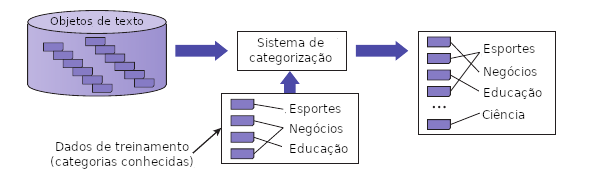
\includegraphics[width=0.75\textwidth]{img/figure15-1-zhai-traduzido.png}
    \end{center}
    \vspace{-0.5cm}
    \legend{\ABNTEXfontereduzida \textbf{Fonte:} Figura adaptada de \citeonline[p.~300]{Zhai2016TDMA}.}
    \label{fig:categorização-de-texto-zhai2016}
\end{figure}
    
    A Mineração de Texto aborda, dentre seus tipos de tarefas oriundas da mineração de dados, a tarefa de classificação nas coleções de documentos, geralmente chamada de classificação de texto ou categorização de texto \cite[p.~35]{Zhai2016TDMA}.
    Classificação é definido como o processo de designar uma ou mais categorias a cada objeto de texto, dentre categorias predefinidas, sendo que predominantemente é utilizado um conjunto de textos já classificados para treinamento \cite[p.~7]{Jo2018TMCIBDC} \cite[p.~299]{Zhai2016TDMA}.
    Esse processo está exemplificado na Figura \ref{fig:categorização-de-texto-zhai2016}.
    
    No processo de classificação de texto são derivados atributos dos objetos de texto originais, um passo necessário para funcionamento do modelo de classificação proveniente da área de aprendizado de máquina \cite[p.~64]{Feldman:2006:TMH:1076381}.
    Diferentes conjuntos de atributos podem impactar diretamente no desempenho de um classificador \cite[p.~304--306]{Zhai2016TDMA}, o qual é tipicamente mensurado pela acurácia\footnotemark{} \cite[p.~313--314]{Zhai2016TDMA} \cite[p.~9]{Jo2018TMCIBDC}.
    
    \footnotetext{Número de previsões corretas dividido pelo número total de previsões feitas \cite[p.~313]{Zhai2016TDMA}.}
    
    A criação de atributos\footnotemark{} é algo que pode melhorar a acurácia dos classificadores utilizados em tarefas de mineração de dados \cite[p.~118]{MaFEDS2018}, os mesmos classificadores também são utilizados em tarefas de Mineração de Texto \cite[p.~1241]{Sammut2017EMLDM}. 
    Portanto, sugerir a criação de novos atributos, e avaliar o impacto destes atributos no desempenho de classificadores, contribui para o refinamento das técnicas de Mineração de Texto.
    Apesar de técnicas de Recuperação de Informação fundamentarem e servirem de base, principalmente, para o pré-processamento dos textos na MT, a utilização de funções de ranqueamento de RI na criação de atributos para MT é recente, sendo encontradas na literatura somente as pesquisas de \citeonline{WEREN_MESTRADO_2014}.
    
    \footnotetext{Processo da área de engenharia de atributos (\textit{feature engineering}), também chamado de extração, ou construção, de atributos \cite[p.~498--503]{Sammut2017EMLDM}.}
    
    A área de Recuperação de Informação abarca os processos de armazenamento, indexação, recuperação e ranqueamento de consultas sobre coleções de documentos \cite[p.~5--8]{Baeza-Yates2011}.
    A RI sempre busca a otimização destes processos, tanto em questão de melhorias na velocidade de resposta, como também na questão da satisfação da necessidade de informação dos usuários dos sistemas de RI \cite[p~.671--672]{Sammut2017EMLDM}, e segundo \citeonline[p.~2, tradução nossa]{KowalskiIRAA201}:
    % \begin{citacao}[english]
        % The overall goal of an Information Retrieval System is to minimize the user overhead in locating the information of value. 
        % Overhead from a user’s perspective can be defined as the time it takes to locate the needed information. 
        % The time starts when a user starts to interact with the system and ends when they have found the items of interest.
    % \end{citacao}
    
    \begin{citacao}
        O objetivo principal de um sistema de Recuperação de Informação é minimizar a sobrecarga do usuário em localizar informação de valor. 
        Na perspectiva do usuário, sobrecarga pode ser definido como o tempo que decorre para localizar a informação necessária.
        O tempo inicia quando um usuário começa a interagir com o sistema e termina quando encontra os itens de interesse.
    \end{citacao}
    Implementações de sistemas de RI que atendam os objetivos da área se tornam complexas por estes sistemas terem que lidar com a integração dos processos de forma a trazer a melhor experiência ao usuário.
    % aqui é a conclusão da parte sobre RI na introdução (após ressaltar sua complexidade):
    Portanto, a utilização de ferramentas que subsidiem as tarefas de armazenamento, indexação, recuperação e ranqueamento da Recuperação de Informação é vantajosa por facilitar a introdução de atributos derivados de RI nas tarefas de MT.
   
    O uso de diferentes ferramentas, para realizar a geração dos mesmos atributos derivados de RI, possibilita ainda a comparação do desempenho dessas ferramentas nas tarefas de indexação e de consulta para o ranqueamento.
    
    
    
    % A área de engenharia de atributos (tradução livre de \textit{feature engineering}) embarca a transformação, geração, extração, seleção, análise e avaliação de atributos para aprendizado de máquina
    
    % Dentre as medidas para 
    

    
    % Sistemas de RI são feitos para armazenar documentos e permitirem a sua consulta por usuários, 

% Definição do Problema
% Complexidade de RI na MT.	Dizer que RI é uma área, e vamos buscar ferramentas que subsidiam o cálculo das variáveis de RI. 

    % \section{Justificativa} \label{sec:Justificativa}
        % Existem poucos estudos na área de utilização de atributos de RI em tarefas de Mineração de Texto, também não existem (pesquisa isso) estudos do desempenho das ferramentas para subsidiar o cálculo das formulas de ranqueamento de RI. 2

    \section{Objetivo geral} \label{sec:Objetivo-geral}
        % Implementar um sistema que possibilite a utilização de atributos gerados a partir da função de ranqueamento BM25 em tarefas de Mineração de Texto.
        % Sugestão de Rosalvo
        Avaliar o desempenho de atributos oriundos de Recuperação de Informação para tarefas de Mineração de Textos.

% Avaliar o desempenho de técnicas de RI como atributos em MT
% Avaliar o desempenho de ferramentas computacionais para construção (indexação) de BDs e criação dos atributos de RI.
% Avaliar o desempenho dos classificadores de MT com e sem as var de RI.

    \section{Objetivos específicos} \label{sec:Objetivos-específicos}
        \begin{itemize}
        	\item Avaliar o ganho de desempenho de classificadores de Mineração de Texto com adição de atributos derivados da função de ranqueamento BM25 da Recuperação de Informação, em pelo menos 2 corpus de competições diferentes, utilizando medidas consolidadas na literatura;
        	
        	\item Reproduzir soluções disponíveis \textit{online} para os corpus selecionados, comprovando as medidas dos resultados das competições;
        	
            \item Elencar em qual dos corpus selecionados os atributos criados proporcionam maior ganho de desempenho de classificador;
            
            \item Comparar o desempenho computacional de ferramentas de armazenamento e indexação de textos:
            \begin{itemize}
                \item na questão de indexação;
                \item na questão de consulta utilizando as implementações do BM25 nativas das ferramentas;
            \end{itemize}
            
            % \item Avaliar, empiricamente, a facilidade de instalação, utilização e integração das ferramentas de armazenamento e indexação selecionadas.
        \end{itemize}
    
    \section{Organização do trabalho} \label{sec:Organização-do-trabalho}
        Este trabalho está dividido em 5 capítulos. 
        O primeiro capítulo foi introdutório e apresentou a motivação para o desenvolvimento desta pesquisa, e qual o problema específico que o projeto aborda.
        
        No segundo capítulo é desenvolvida a fundamentação teórica dos principais campos de abordagem, sendo realizadas revisões bibliográficas das áreas de Recuperação de Informação e de Mineração de Texto.
        
        O terceiro apresenta a metodologia para execução do projeto, ilustrada por meio de um diagrama, que é logo em seguida detalhado textualmente, e os tópicos principais são expandidos em subseções.
        % No final do capítulo um cronograma de execução é apresentado, feito com base nos dias letivos do Calendário Acadêmico 2019 da UNIVASF.

        Detalhes da configuração experimental, da execução da pesquisa e os resultados obtidos são apresentados, e brevemente discutidos, no quarto capítulo. 
        A disposição dos resultados é feita por meio da tabulação dos dados e também disposição em gráficos.

        O quinto e último capítulo traz as considerações finais e visiona trabalhos futuros.
% \lipsum[10-12]

		%--------------------------------------------------------------------------------------
% Este arquivo contém a sua fundamentação teórica
%--------------------------------------------------------------------------------------
\chapter{Fundamentação teórica} \label{ch:FundamentaçãoTeórica}
    A utilização de funções de ranqueamento da Recuperação de Informação engloba o conhecimento a cerca de fundamentos da área que serão abordados na primeira seção a seguir, a Seção \ref{sec:RecuperaçãoInformação}, que trata desde o surgimento da área até sua evolução para os métodos probabilísticos culminando na função de ranqueamento BM25.

    Para a criação de atributos em tarefas de Mineração de Texto é necessário entender o processo de descoberta do conhecimento da Mineração de Dados, as peculiaridades para criação destes atributos, e ainda métodos de avaliação dos atributos criados. Isto é feito na Seção \ref{sec:MineraçãoTexto}.

    \section{Recuperação de Informação} \label{sec:RecuperaçãoInformação}
% Falar da recuperação de informação com conceito humano

% Estrutura

% - Histórico de RI, explicando o surgimento de métodos de RI com as bibliotecas

    A busca por informação é uma necessidade humana, e uma das principais maneiras de obtê-la é consultar outras pessoas.
    No entanto, devido ao grande acúmulo de informação das sociedades, uma pessoa não pode carregar consigo todo o conhecimento do mundo.
    Assim, um modo considerado primordial de transferir esse conhecimento, que tratamos aqui como informação, é por meio de registros físicos em papel, livros e similares \cite[p.~1]{Grossman2004IRAH}.
    
    No processo de organização desses registros físicos, é notória a função dos bibliotecários de separar os vários tipos de conhecimento que os mais diversos livros podem abrigar e, portanto, os sistemas de classificação de áreas e subáreas do conhecimento são um auxílio para as necessidades de busca por informação que uma pessoa pode ter \cite[p.~1]{Manning2008IIR} \cite[p.~1446]{Sanderson2012THIRR} \cite[p.~6]{Baeza-Yates1999}. 
    % OU  subáreas do conhecimento são uma ferramenta crucial na busca de informações.
    Esses sistemas de classificação facilitam a localização de informações específicas a partir de uma pergunta que uma pessoa pode fazer, mas é necessário saber como o sistema de classificação funciona para que o usuário possa tentar saciar sua necessidade, ou pelo menos será necessário um especialista no sistema (o bibliotecário) para lhe guiar.
    E mesmo assim, depois de adquirir os diversos materiais que podem responder à sua pergunta, esta pessoa ainda terá que conferir nos textos se estes satisfazem sua necessidade.
    
    % - RI em equipamentos eletromecânicos no início do século 20
    % -- O que fez surgir esses sistemas, a necessidade
    
    Os sistemas de classificação manual se mostram ineficazes devido ao surgimento crescente e constante de novas informações \cite[p.~6]{Baeza-Yates1999} desde o início do século 20. 
    Desta maneira, além da imensidão de novas pesquisas científicas sendo publicadas, livros surgindo, entre outros registro históricos, que precisam ser classificados, existe também o problema da classificação não poder abranger todo tipo de necessidade que tal material pode satisfazer \cite[p.~1444]{Sanderson2012THIRR}. 
    A preocupação com sistemas que possam indexar todo esse material e fornecer um acesso rápido às necessidades de informação de uma pessoa surgiu também no início do século 20 \cite{Bush:1979:WMT:1113634.1113638}, onde sistemas mecânicos de recuperação de informação foram visionados.
    
    
    % - A área de pesquisa de RI que surgiu com a utilização de computadores para indexar informação
    % -- A utilização de computadores para fazer o serviço de RI
    
    A partir da criação de sistemas computacionais na década de 1940, foi vista a possibilidade de criação de sistemas que armazenassem informações e possibilitassem essa consulta rápida sobre as informações armazenadas, sendo necessários estabelecer algoritmos que retornassem informação relevante ao que o usuário do sistema procura. 
    Tendo então nesse momento o início do campo científico de Recuperação de Informação (RI, do inglês \textit{Information Retrieval}) que é encontrar material (geralmente documentos) de natureza desestruturada (geralmente texto) que satisfaça uma necessidade de informação dentro de grandes acervos (geralmente armazenados em computadores) \cite[p.~1]{Manning2008IIR}.
    
    A lei de Moore diz que o crescimento da velocidade de processamento é contínuo, e similarmente existe uma duplicação constante da capacidade de armazenamento digital a cada dois anos. % CARECE DE FONTES - Preciso procurar
    Logo, a necessidade de sistemas de Recuperação de Informação surge do crescimento exponencial das coleções de informação derivadas do crescimento de armazenamento, e consequente inabilidade das técnicas tradicionais de catalogação de lidar com isso \cite{Sanderson2012THIRR}.
    Ter um amontoado de conhecimento, informação, e não poder acessar o que é relevante de modo rápido não é interessante pois assim o desenvolvimento de pesquisas, por exemplo, fica comprometido e pode perder relevância \cite{Bush:1979:WMT:1113634.1113638}.
    
    % -- Conceitos fundamentais de RI
    A RI como uma disciplina de pesquisa se iniciou no final da década de 50 a partir do uso de computadores na busca de referências de texto associadas com um assunto \cite[p.~3]{Sanderson2012THIRR}, as preocupações iniciais dessa área eram 
    \begin{enumerate*}[label=(\alph*)]
    \item \textit{como indexar documentos} e \item \textit{como recuperá-los},
    \end{enumerate*}
    sendo a busca da melhor maneira de executar tais tarefas o principal objetivo da RI.
    
    Logo no início do seu desenvolvimento as técnicas de RI buscaram se basear em sistemas existentes já consolidados no campo bibliotecário para indexar coleções de itens, tendo como uma técnica de abordagem clássica atribuir códigos numéricos a essas coleções, como por exemplo o feito pelo sistema de Classificação Decimal de Dewey \cite[p.~1446]{Sanderson2012THIRR}.
    No entanto foi demonstrado por \citeonline{Cleverdon1959TESUIR} que um sistema baseado em palavras, como o sistema Uniterm proposto por \citeonline{Taube1952UTCI}, era tão bom e até melhor que outras abordagens clássicas, sendo a indexação por palavras posteriormente adotada pelos sistemas de RI \cite[p.~1446]{Sanderson2012THIRR}.
    
    Um exemplo do funcionamento de um sistema moderno de RI pode ser visto na Figura \ref{fig:diagrama-baeza2013-fig1-3}, onde está apresentado um fluxograma dos processos de indexação, recuperação, e ranqueamento de documentos. 
    Sendo o ranqueamento feito por sistemas de RI o interesse deste trabalho, alguns dos termos apresentados nessa figura serão abordados logo mais.
    
    \begin{figure}[h]
    \centering
    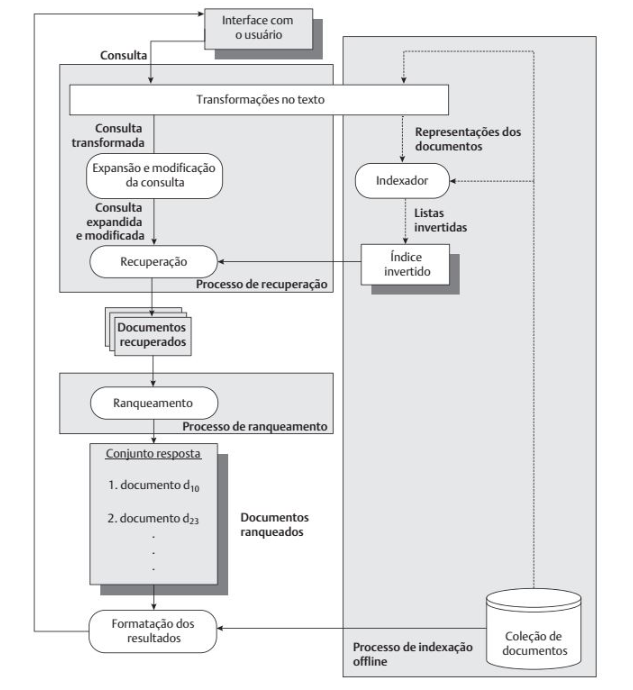
\includegraphics[width=0.85\textwidth]{img/baeza2013-figura-1-3.png}
    \caption{Processos de indexação, recuperação, e ranqueamento dos documentos. Figura extraída de \citeonline[p.~8]{Baeza-Yates2011}.}
    \label{fig:diagrama-baeza2013-fig1-3}
\end{figure}
    
    Segundo \citeonline[p.~7]{Baeza-Yates2011} a arquitetura de funcionamento de um \textit{software} de RI inicia com o processo de indexação executado \textit{offline}, antes do sistema estar pronto para processar consultas, e a estrutura de indexação mais popular é a chamada de índice invertido.
    Após a indexação da coleção de documentos, então o sistema está preparado para o processo de recuperação, onde o usuário especifica sua consulta, a qual é modificada pelo sistema para ficar mais próxima do sistema de indexação utilizado.
    A consulta modificada é utilizada para obter o conjunto de documentos recuperados, os quais, idealmente, satisfazem as necessidades de informação do usuário.
    Por fim, os documentos recuperados são ranqueados pela sua pertinencia de relevância para o usuário.
    
    % -- Os primeiros sistemas de RI, booleanos 
\subsection{Métodos booleanos} \label{subsec:MétodosBooleanos}

    Uma consulta (chamada de \textit{query}) representa uma necessidade de informação a ser saciada por um sistema de RI, e essa consulta é composta de termos (um sinônimo para palavras) que nos primeiros desses sistemas era limitada a combinações lógicas e eram recuperados os documentos que tinham correspondência exata com ela \cite[p.~1446]{Sanderson2012THIRR}. 
    Este método de recuperação de informação é conhecido como recuperação booleana, e para indexar os documentos é utilizada, geralmente, uma matriz binária de incidência de termo-documento. 
    Exemplificamos uma matriz dessas na Tabela \ref{tab:matriz-incidência-termo-documento}, que é o exemplo dado por \citeonline[p.~3--4]{Manning2008IIR} de uma matriz de incidência de termo-documento para o livro \textit{Shakespeare’s Collected Works}, que reúne as obras completas de Shakespeare.

    \input{tex/table/matriz-incidencia-termo-documento.tex}
% \clearpage
    
    % -- A pesquisa de RI sendo desenvolvida, citar sistemas rankeados
    \subsection{Ranqueamento} \label{subsec:Ranqueamento}
Devido à limitação dos métodos booleanos de somente retornar resultados conforme a presença ou não dos termos da consulta nos documentos \cite[p.~100]{Manning2008IIR}, foi proposto em 1957 por Luhn e 1959 por Maron \textit{et al.} uma abordagem de recuperação ranqueada \cite[p.~1446]{Sanderson2012THIRR} a qual, em contraste com recuperação booleana, baseada nos termos de consulta estabelecia uma pontuação para cada artigo de modo probabilístico e retornava os artigos de modo ordenado e demonstraram que essa técnica sobressaía a recuperação booleana.

% Explicar o funcionamento de uma recuperação ranqueada, como é feito esse ranqueamento?
O procedimento fundamental para ranqueamento dos documentos, conforme os termos de consulta, consiste na atribuição de pontuação aos documentos a partir da contabilização do número de aparições (chama de frequência) de cada um dos termos no documento.
Essa pontuação é calculada considerando que além da frequência do termo, denotada como $\text{tf}_{\text{\textit{t},\textit{d}}}$ que é o número de ocorrências do termo \textit{t} em um documento \textit{d}, existe também a sua relevância, que depende do número de aparições do termo na coleção de documentos inteira.
Quanto mais um termo aparece na coleção menos relevante ele é, e este valor de relevância é denotado por $\text{idf}_{\text{\textit{t}}}$ que é o inverso da frequência de um termo \textit{t} em uma coleção de documentos.
Segundo \citeonline[p.~108]{Manning2008IIR} este valor da relevância é calculado do seguinte modo:

\begin{equation}
    \text{idf}_{\text{\textit{t}}} = \log{\frac{N}{\text{df}_{\text{\textit{t}}}}}.
\end{equation}

O valor resultante da relação entre a frequência do termo e o inverso da frequência nos documentos é chamado de $\text{tf-idf}_{\text{\textit{t},\textit{d}}}$ (\textit{term frequency-inverse document frequency}), sendo este valor um dos pesos mais utilizados para ranqueamento \cite[p.~107--110]{Manning2008IIR}, e é calculado  como segue:
\begin{equation}
    \text{tf-idf}_{\text{\textit{t},\textit{d}}}  = \text{tf}_{\text{\textit{t},\textit{d}}} \times \text{idf}_{\text{\textit{t}}}.
\end{equation}

\input{tex/table/tf-idf-exemplo.tex}

Na Tabela \ref{tab:exemplo-tf-idf} temos um exemplo de cálculo dos valores de tf-idf para posterior cálculo da pontuação para ranqueamento, conforme alguma determinada consulta. 
A pontuação de um documento \textit{d} é a soma dos pesos de tf-idf de cada termo \textit{t} em \textit{d}, sendo os termos \textit{t} presentes na consulta realizada \cite[p.~109]{Manning2008IIR}, representamos esse cálculo do seguinte modo:

\begin{equation}
    \label{eq:pontuação-simples-tf-idf}
    \text{Pontuação(\textit{q},\textit{d})} = \sum_{\textit{t} \in \textit{q}}^{} \text{tf-idf}_{\text{\textit{t},\textit{d}}}.
\end{equation}

% Quando uma consulta é feita são utilizados os valores 
% (onde Pontuação({\textit{auto},\textit{car}},DocX))  

Utilizando a Equação \ref{eq:pontuação-simples-tf-idf} uma consulta com os termos \textit{auto car} retornaria no seu ranqueamento os documentos com a seguinte pontuação, calculamos Pontuação(\{\textit{auto},\textit{car}\},DocX) para cada documento, por exemplo:
\begin{itemize}
    \setlength\itemsep{-0.2em}
    \item Doc1: 50,79
    \item Doc2: 75,24
    \item Doc3: 39,60
\end{itemize}

A ordenação dos documentos apresentados como resultado à consulta \textit{auto car} seria então a seguinte: 1\textordmasculine{} - Doc2; 2\textordmasculine{} - Doc1; e 3\textordmasculine{} - Doc3, que se observamos a Tabela \ref{tab:exemplo-tf-idf} é um bom resulto já que o Doc2 contém uma grande frequência do termo \textit{auto} e o Doc3 não possui este termo.


Ao longo dos anos foi demonstrada a superioridade da recuperação ranqueada sobre a recuperação booleana \cite{Jones:1981:IRE:539571}, e são as técnicas de recuperação ranqueadas que trazem maior interesse para a área de Mineração de Textos, em específico estamos interessados nos modelos vetoriais e os modelos probabilísticos de RI que são evoluções da recuperação ranqueada.
% ESTOU PENSANDO EM JÁ CITAR O BM25 no parágrafo acima.
% -- Em algum ponto mencionar que Recuperação de Informação (Information Retrieval) não deve ser confundido com Procura de Informação (Information Search), pois a Procura de Informação é o campo que estuda a interação das pessoas com sistemas de recuperação de informação.




    \newpage

    \section{Mineração de Texto} \label{sec:MineraçãoTexto}
    % Introdução a Mineração de Texto
    % - Falar de IA?
    % -- Surgimento do processo de KDD
    % -- É um subramo do KDD, KDT
    A Mineração de Textos (MT) é definida como o processo de extrair conhecimento implícito de dados textuais \cite{Jo2018TMCIBDC,Feldman:2006:TMH:1076381} e por isso é às vezes tratada como \textit{knowledge discovery in text} (livremente traduzido para descoberta de conhecimento em texto) \cite{Kodratoff:1999:KDT:646358.689959, Feldman:1995:KDT:3001335.3001354}, sendo análogo ao termo \textit{knowledge discovery in data} (KDD) que se refere à Mineração de Dados, ramo da Inteligência Artificial que dá suporte à MT. 
    Apesar de haver um uso sinônimo entre Mineração de Dados e KDD, alguns autores tratam a Mineração de Dados como somente uma parte desse processo de descoberta de conhecimento \cite[p.~6]{Han:2011:DMC:1972541}, sendo este um processo iterativo, conforme ilustrado na Figura \ref{fig:diagrama-mineração-texto-han}, composto pelas seguintes fases (ou etapas) segundo \citeonline[p.~6--7]{Han:2011:DMC:1972541}:
    % - Passos da MT
    % 1. Data cleaning (to remove noise and inconsistent data)
    % 2. Data integration (where multiple data sources may be combined)3
    % 3. Data selection (where data relevant to the analysis task are retrieved from the  database)
    % 4. Data transformation (where data are transformed and consolidated into forms appropriate for mining by performing summary or aggregation operations)4
    % 5. Data mining (an essential process where intelligent methods are applied to extract data patterns)
    % 6. Pattern evaluation (to identify the truly interesting patterns representing knowledge  based on interestingness measures—see Section 1.4.6)
    % 7. Knowledge presentation (where visualization and knowledge representation techniques are used to present mined knowledge to users)
    \begin{enumerate}
        \item \textbf{Limpeza dos dados}: remoção de ruído e dados inconsistentes;
        \item \textbf{Integração dos dados}: combinação de múltiplas fontes de dados;
        \item \textbf{Seleção dos dados}: dados relevantes para a tarefa de análise são recuperados do banco de dados;
        \item \textbf{Transformação dos dados}: dados são transformados e consolidados em formas apropriadas para mineração sendo realizadas, por exemplo, ações de agregação ou resumo;
        \item \textbf{Mineração dos dados}: métodos inteligentes são aplicados para extrair padrões de dados;
        \item \textbf{Avaliação de padrões}: são identificados os padrões que realmente tão interessantes para representar o conhecimento baseado em medidas de nível de interesse;
        \item \textbf{Apresentação do conhecimento}: o conhecimento minerado é apresando aos usuários por meio de técnicas de visualização e representação de conhecimento.
    \end{enumerate}
    % Certainly, text mining derives much of its inspiration and direction from seminal research on data mining. Therefore, it is not surprising to find that text mining and data mining systems evince many high-level architectural similarities. 
    
    \begin{figure}[ht]
    \centering
    \caption{Mineração de dados como uma fase do processo de descoberta do conhecimento (KDD).}
    \begin{center}
        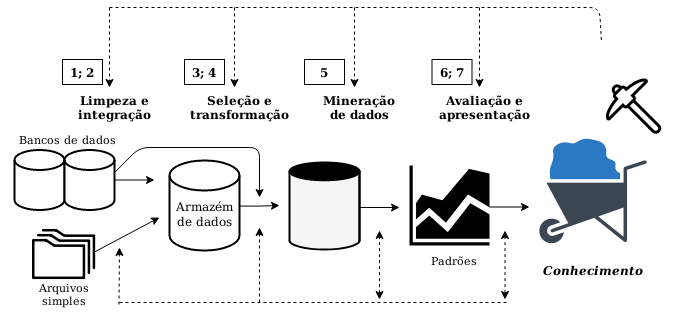
\includegraphics[width=0.85\textwidth]{img/based-on-figure-1-4-han-2011.png}
    \end{center}
    \vspace{-0.5cm}
    \legend{\ABNTEXfontereduzida \textbf{Fonte:} Figura baseada na original de \citeonline[p.~7]{Han:2011:DMC:1972541}.}
    \label{fig:diagrama-mineração-texto-han}
\end{figure}
    
    É importante notar essas 7 etapas de desenvolvimento de Mineração de Dados para abordamos a definição de MT, pois esta deriva muitas técnicas desenvolvidas na pesquisa do campo de Mineração de Dados para seu campo de aplicação, logo sistemas baseados em ambas áreas vão apresentar similaridades estruturais \cite[p.~1]{Feldman:2006:TMH:1076381}. 
    
    % Text mining can be broadly defined as a knowledge-intensive process in which a user interacts with a document collection over time by using a suite of analysis tools. In a manner analogous to data mining, text mining seeks to extract useful information from data sources through the identification and exploration of interesting patterns.
    
    % Because data mining assumes that data have already been stored in a structured format, much of its preprocessing focus falls on two critical tasks: Scrubbing and normalizing data and creating extensive numbers of table joins. In contrast, for text mining systems, preprocessing operations center on the identification and extraction of representative features for natural language documents. These preprocessing operations are responsible for transforming unstructured data stored in document collections into a more explicitly structured intermediate format, which is a concern that is not relevant for most data mining systems.
    
    A Mineração de Dados assume que os dados, que vão ser tratados durante seu processo, já foram armazenados em um formato estruturado, logo a maior parte de seu pré-processamento vai estar ligado às etapas 1 e 2 do processo de KDD citado, as de limpeza e integração dos dados \cite[p.~1]{Feldman:2006:TMH:1076381}. % Talvez seja necessário ao falar de linguagem natural dar um exemplo e um contra exemplo? Português e Java?
    Já na MT, como os dados de trabalho são textos, sendo texto configurado como dados desestruturados que consistem de \textit{strings} (palavras) organizadas de forma coerente e sendo pertencentes a uma linguagem natural \cite[p.~1]{Jo2018TMCIBDC}, temos que as operações de pré-processamento vão estar mais focadas em etapas adicionais, prévias às citadas para o processo de KDD, sendo estas novas direcionadas à identificação e extração de \textit{features} (atributos) representativas para documentos escritos em linguagem natural, transformando os dados não estruturados, que estão armazenados em coleções de documentos, em um formato mais explicitamente estruturado \cite[p.~1]{Feldman:2006:TMH:1076381}.
    % Text is defined as the unstructured data which consists of strings which are called words [82]
    
    
    % Na década de 70 houve o surgimento de diversas técnicas de gerenciamento de banco de dados, como por exemplo a 
    
    % -- Utiliza de várias áreas, falar delas
    % -- Utiliza das técnicas de RI para indexar os textos em algumas de suas aplicações
    % Text mining preprocessing operations include a variety of different types of techniques culled and adapted from information retrieval, information extraction, and computational linguistics research that transform raw, unstructured, original-format content (like that which can be downloaded from PubMed) into a carefully structured, intermediate data format. Knowledge discovery operations, in turn, are operated against this specially structured intermediate representation of the original document collection.
    
    As operações de pré-processamento para MT utilizam de várias técnicas adaptadas dos campos de Recuperação de Informação, extração de informação e linguística computacional para transformar as coleções de documentos desestruturados em dados intermediários cuidadosamente estruturados \cite[p.~2--3]{Feldman:2006:TMH:1076381}. 
    Essa estrutura intermediária é definida por um modelo representacional dos documentos de texto composto por um conjunto de atributos, sendo sempre preferidos os modelos com menor número de variáveis significativas para a representação \cite[p.~4]{Feldman:2006:TMH:1076381}.
    % In Table 1.1, the differences between the mining and the retrieval are presented. The output of data mining is the implicit knowledge which is necessary directly for making decisions, whereas that of retrieval is some of data items which are relevant to the given query. For example, in the domain of stock prices, the prediction of future stock prices is a typical task of data mining, whereas taking some of past and current stock prices is that of information retrieval. Note that the perfect certainty never exists in the data mining, compared to the retrieval. The more advanced computation for making knowledge from the raw data, which is called synthesis, is required for doing the data mining tasks.
    
    Apesar da Mineração de Texto utilizar de técnicas da Recuperação de Informação, ambos são campos independentes com objetivos diferentes conforme ressalta \citeonline[p.~4, tradução nossa]{Jo2018TMCIBDC} (apresentados de modo resumido na Tabela \ref{tab:mineração-vs-recuperação}):

    \begin{citacao}
        A saída da mineração de dados é o conhecimento implícito que é necessário diretamente para a tomada de decisões, enquanto a saída da recuperação é composta por alguns dos itens de dados que são relevantes para a consulta dada. 
        Por exemplo, no domínio de preços de ações, a previsão dos preços futuros de ações é uma tarefa típica da mineração de dados, enquanto que obter alguns dos preços de ações passadas e atuais é tarefa da recuperação de informação. 
        Observe que a certeza perfeita nunca existe na mineração de dados, em comparação com a recuperação. 
        A computação mais avançada para obter conhecimento dos dados brutos, chamada de síntese, é necessária para executar as tarefas de mineração de dados.
    \end{citacao}
    
    \begin{table}[H]
    \centering
    \caption{Mineração de Dados versus Recuperação de Informação (em específico para objetos de texto a comparação vale para Mineração de Texto versus Recuperação de Texto).}
    \begin{tabular}{|l|l|l|}
        \hline
         
        & \makecell[l]{\textbf{Mineração}}
        & \makecell[l]{\textbf{Recuperação}}
        \\ \hline
        Saída
        & Conhecimento 
        & Itens relevantes
        \\ \hline
        Exemplo
        & Valores previstos 
        & Valores anteriores ou atuais
        \\ \hline
        Certeza
        & Probabilística 
        & Nítida
        \\ \hline
        Síntese
        & Necessária 
        & Opcional
        \\ 
        \hline
    \end{tabular}
    \legend{\ABNTEXfontereduzida \textbf{Fonte:} \citeonline[p.~4]{Jo2018TMCIBDC}}
    \label{tab:mineração-vs-recuperação}
\end{table}
    % Ressaltar denovo o suporte que a RI dá à MT, e então apresentar a diferenciação que Jo2018 faz na tabela 1.1 pag 4, e talvez a perspectiva do usuário apresentada por Zhai2016 a qual diferencia a Recuperação de Informação como Acesso dando poder de Selecionar Informação, e Mineração de Texto como Mineração possibilitando Criar Conhecimento, ele ainda apresenta a parte da Clusterização como Organização possibilitando Adicionar Estruturas/Marcações
    % Pensei em aqui contextualizar um pouco sobre os diversos campos que dão suporte ao KDD (Mineração de Dados) e à MT e colocar uma imagem parecida com a do \cite{Han:2011:DMC:1972541} na página 23 para mostrar os campos que dão suporte a MT
    
    A definição dos atributos para MT busca tirar proveito dos mais variados elementos presentes em um documento escrito em linguagem natural, no entanto é necessário um cuidado pois existe um grande número de palavras, frases e outros artefatos que podem comprometer o desempenho de um sistema de Mineração de Texto ou tornar a tarefa infactível \cite[p.~4]{Feldman:2006:TMH:1076381}, por isso a necessidade de identificar os melhores atributos, que trazem mais informação sobre o texto. 
    Nesse ponto que a MT pode se auxiliar de técnicas de RI para incrementar seu grupo de atributos, sendo alguns, como por exemplo o BM25 para RI ranqueada, utilizadas em competições de identificação de perfil de autores \cite{WEREN_MESTRADO_2014,WEREN_CLEF_2014,WEREN_ARTIGO_2014}. % procurar outros!!!!!.
    
    % -- Já devo diferenciar aqui
    
    % Falta falar de:
    % * Feature Engineering
    %  ---> Falar da definição mais ampla, feature selection, extraction, etc.
    % * Medidas de avaliação
    
    \subsection{Corpus} \label{subsec:Corpus}
    % Jo2018 - página 6 TEXT FORMATS
        Vários formatos de texto são utilizados para o processamento computacional de texto, segundo \citeonline[p.~6]{Jo2018TMCIBDC} os mais populares são os distribuídos pelo \textit{software} MS Office, como o arquivo padrão do MS Word com extensão ``doc'', MS PowerPoint com extensão ``ppt'', e o MS Excel com o ``xls'', e ainda para transferência entre computadores o mais utilizado é o formato PDF (\textit{Portable Documento Format}).
        
        \begin{figure}[ht]
    \centering
    \caption{Arquivo de texto simples, texto não formatado, aberto para edição no xed.}
    \begin{center}
        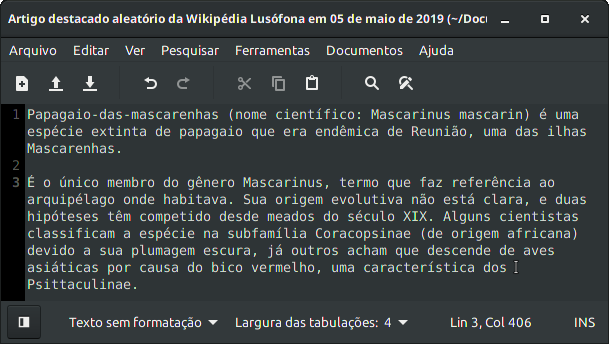
\includegraphics[width=0.75\textwidth]{img/exemplo-texto-simples.png}
    \end{center}
    \vspace{-0.5cm}
    \legend{\ABNTEXfontereduzida \textbf{Fonte:} O autor, conteúdo do texto obtido de \citeonline{Wikipedia_ConteudoDest05maio_2019}.}
    \label{fig:exemplo-texto-simples}
\end{figure}


        
        O texto simples, ou texto sem formatação, é o formato mais elementar de texto que é feito por um editor de texto, exemplificado na Figura \ref{fig:exemplo-texto-simples} por um arquivo aberto no editor xed\footnote{xed é um editor de texto leve e pequeno feito para o X-Apps \cite{LinuxMintXed2019}.}.
        Usualmente cada texto corresponde a único arquivo, sendo geralmente armazenado com a extensão ``txt'' nos sistemas operacionais Windows \cite[p.~6]{Jo2018TMCIBDC}.
        
        O XML (\textit{Extensive Markup Language}) pode ser considerado como outro formato de texto conforme exibido na Figura \ref{fig:exemplo-arquivo-xml}. 
        É o formato de documento \textit{web} mais flexível e foi projetado com base no HTML, o XML 1.0 foi padronizado pela W3C (\textit{World Wide Web Consortium}) em sua primeira versão em 1998, sendo a quinta edição a mais recente publicada em novembro de 2008 \cite{XML10_5ed_2008}.
        Atualmente o XML é utilizado como padrão para descrever itens de dados textuais de forma relacional, onde cada campo possui uma etiqueta de início e de fim, e o valor do campo fica entre estas etiquetas \cite[p.~6]{Jo2018TMCIBDC}.
        
        \begin{figure}[ht]
    \centering
    \caption{Exemplo de documento XML aberto no editor xed.}
    \begin{center}
        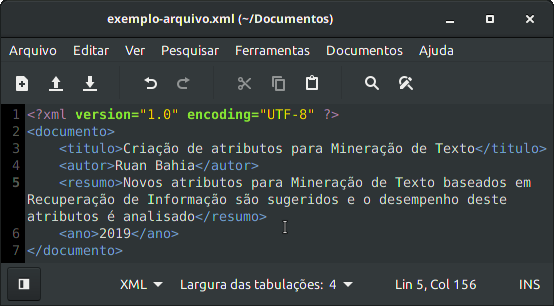
\includegraphics[width=0.65\textwidth]{img/exemplo-arquivo-xml.png}
    \end{center}
    \vspace{-0.5cm}
    \legend{\ABNTEXfontereduzida \textbf{Fonte:} O autor.}
    \label{fig:exemplo-arquivo-xml}
\end{figure}
        
        Uma coleção de textos simples é chamada de corpus, geralmente sendo referenciado pelo diretório que contém os arquivos de texto, e excepcionalmente um único arquivo pode também corresponder a um corpus ao invés de ser somente um único arquivo de texto \cite[p.~6]{Jo2018TMCIBDC}.
        Num conceito mais abrangente, \citeonline[p.~9]{KwartlerTMPWR2017} considera como corpus qualquer corpo, ou conjunto, grande de texto organizado, assim um conjunto de arquivos de texto XML também é tratado como um corpus.
    
    \subsection{Tarefas de Mineração de Dados} \label{subsec:Tarefas-de-Mineração-de-Dados}
        As tarefas de Mineração de Dados podem ser divididas em duas categorias, segundo \citeonline[p.~7]{TanIDM2014} e \citeonline[p.~15]{Han:2011:DMC:1972541}: 
        \begin{itemize}
            \item \textbf{Descritivas}: tem como objetivo caracterizar propriedades dos dados no conjunto objetivo por meio da derivação de padrões que resumem as relações nos dados; e
            
            \item \textbf{Preditivas}: realizam uma indução nos dados presentes objetivando prever valores de um atributo em particular, sendo este atributo a ser previsto chamado de objetivo. 
        \end{itemize}
        
        Quanto às tarefas em si, a mineração de dados possui tarefas de agrupamento, associação, classificação, descrição, detecção de anomalias, e de regressão.
        As quatro principais estão ilustradas na Figura \ref{fig:tarefas-principais-mineração-dados}.
        As tarefas de classificação e de regressão entram na categoria de tarefas preditivas, e são às vezes referidas como tarefas de modelagem preditiva. 
        Ainda, tarefas de classificação trabalham com atributos objetivos discretos, enquanto que tarefas de regressão tem seus atributos objetivos como variáveis contínuas \citeonline[p.~7--8]{TanIDM2014}, e ambas focam na análise de conjuntos de dados rotulados, os chamados de conjuntos de treinamento \cite[p.~19]{Han:2011:DMC:1972541}.
        Na Mineração de Textos uma tarefa de classificação normalmente recebe o nome de \textbf{categorização de texto} \cite[p.~6]{TurchiATPUKM2009} \cite[p.~61]{Feldman:2006:TMH:1076381}.
        
        \begin{figure}[ht]
    \centering
    \caption{As quatro principais tarefas da mineração de dados.}
    \begin{center}
        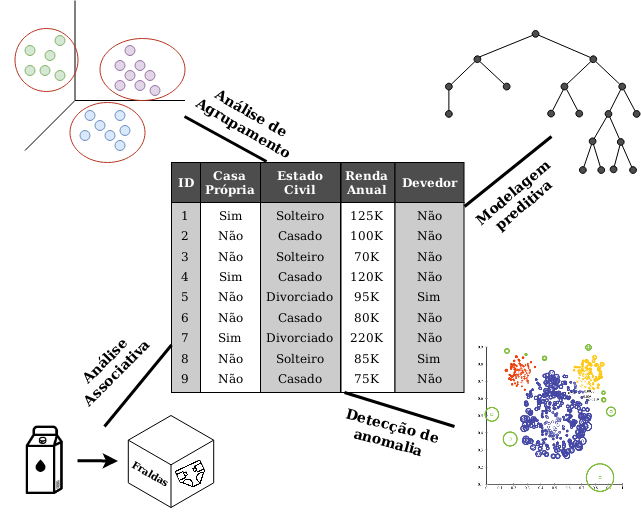
\includegraphics[width=0.85\textwidth]{img/tarefas-principais-mineracao-dados.png}
    \end{center}
    \vspace{-0.5cm}
    \legend{\ABNTEXfontereduzida \textbf{Fonte:} Figura baseada na original de \citeonline[p.~7]{TanIDM2014}.}
    \label{fig:tarefas-principais-mineração-dados}
\end{figure}


        
        Segundo os autores \citeonline[p.~15--21]{Han:2011:DMC:1972541}, \citeonline[p.~8--11]{TanIDM2014} e \citeonline[p.~8--14]{LaroseDKD2014} as demais tarefas da mineração de dados são descritivas e podem ser caracterizadas como segue:
        \begin{itemize}
            \item \textbf{Agrupamento}: consiste numa análise dos dados sem consulta à rótulos de classe, podendo estes até não estarem presentes, e este tipo de tarefa é utilizado para gerar rótulos de classes para grupos de dados. 
            Na literatura é mais comum se referir ao termo em língua inglesa, \textit{clustering};
            
            \item \textbf{Associação}: são descobertos relacionamentos mais frequentes entre os atributos, utilizada para descoberta de padrões, geralmente por meio de regras de implicação;
            
            \item \textbf{Descrição}: os dados são associados com conceitos, consistindo da caracterização dos dados, onde é feita o resumo das características gerais de uma classe objetivo; 
            ou da discriminação dos dados, onde é feita a comparação, contraste, dos atributos de uma classe objetivo com um conjunto de outras classes;
            
            \item \textbf{Detecção de anomalias}: também chamado de detecção de dados discrepantes (\textit{outliers}), foca na identificação de exemplos dos dados que possuem características significativamente diferentes do restante. 
            Muitos métodos de mineração de dados descartam os \textit{outliers} por considerarem estes como ruídos nos dados.
        \end{itemize}
    
        \subsubsection{Classificação binária} \label{subsubsec:Classificação-binária}
            O problema da classificação consiste na aprendizagem da estrutura dos exemplos do conjunto de dados, os quais estão classificados em grupos chamados de categorias ou classes \cite[p.~285]{Aggarwal_DMTT_2015}.
            A entrada consiste de uma coleção de registros, conhecidos como exemplos, cada um caracterizado pela tupla $(\textbf{x},y)$ onde $\textbf{x}$ é um conjunto de atributos e \textit{y} é o atributo chamado de rótulo da classe.
            \citeonline[p.~146, tradução nossa]{TanIDM2014} dizem que ``classificação é a tarefa de aprender uma função objetivo $f$ que mapeia cada conjunto de atributos $x$ a um rótulo de classe predefinido $y$''.
        % Definition 4.1 (Classification). Classification is the task of learning a target function f that maps each attribute set x to one of the predefined class labels y.
        % The target function is also known informally as a classification model. A classification model is useful for the following purposes.
        
            O aprendizado da função objetivo é feito com um modelo, chamado de modelo de treinamento, pois este é baseado no conjunto de treinamento. 
            Então, este modelo de treinamento é utilizado para prever a classe de exemplos não vistos anteriormente, isso quer dizer que estes exemplos não fazem parte do conjunto de treinamento.
            Segundo \citeonline[p.~286, tradução nossa]{Aggarwal_DMTT_2015}, então, a maior parte dos algoritmos de classificação possui duas fases:
            \begin{enumerate}
                \item \textbf{Fase de treinamento}: nesta fase um modelo de treinamento é construído a parte das instâncias de treinamento. Isto pode ser entendido, intuitivamente, como um resumo do modelo matemático dos grupos rotulados no conjunto de dados de treinamento;
                
                \item \textbf{Fase de teste}: nesta fase o modelo de treinamento é utilizado para determinar os rótulos de classe (ou identificadores de grupos) de uma ou mais instâncias não vistas.
            \end{enumerate}
                
            A tarefa de classificação é também chamada de aprendizado supervisionado porque exemplos dos dados são utilizados para aprender as estruturas de agrupamento das classes \cite[p.~285]{Aggarwal_DMTT_2015}.
            Técnicas de classificação são mais apropriadas para dados com categorias binárias ou nominais, não sendo indicados para categorias com significado ordinal, pois a tarefa de classificação não considera a ordem implícita entre as categorias \cite[p.~147]{TanIDM2014}.
            A tarefa de categorização dos dados pode ser com rótulo único ou com múltiplos rótulos, onde na categorização com múltiplos rótulos as categorias se sobrepõem, e já na categorização com rótulo único cada exemplo de dado pertence a exatamente uma categoria \cite[p.~67]{Feldman:2006:TMH:1076381} \cite[p.~306]{TanIDM2014}.
            
            A classificação binária é um caso especial da categorização de rótulo único na qual quantidade de categorias é dois, sendo este o caso mais simples das tarefas de classificação, pois nele só existem duas possibilidades de rótulo de classe e cada objeto de dados pertence, exclusivamente, a uma das classes \cite[p.~67]{Feldman:2006:TMH:1076381} \cite[p.~81]{Jo2018TMCIBDC}.
            Um exemplo clássico de categorização binária de texto é um analisador de \textit{spam}\footnote{Conteúdo indesejado, tratado como lixo eletrônico.} para e-mails, nele só existem duas possibilidades de classificação para dado e-mail, ou \textbf{é \textit{spam}} ou \textbf{não é \textit{spam}}.
        
    \subsection{Engenharia de atributos} \label{subsec:Engenharia-de-atributos}
        % Falar do sentido amplo da feature engineering, abrangindo feature extraction, creation, selection, etc.
        O processo para extrair atributos passíveis de serem utilizados por classificadores da mineração de dados é chamado por \citeonline{ZhengFEML2018} de \textit{feature engineering}, que em uma tradução livre tentando preservar o contexto pode ser chamado de \textit{manejo de atributos}.
        Num conceito mais generalista, \citeonline[p.~3, tradução nossa]{DongFEMLDA2018} define \textit{feature engineering} como uma área que abrange ``os tópicos de transformação de atributos, geração de atributos, extração de atributos, seleção de atributos, análise e avaliação de atributos, metodologias de manejo generalista e automatizado de atributos, e aplicações do manejo de atributos'', sendo esta a definição de engenharia de atributos no processo de KDD.
        
        Cada um dos tópicos da engenharia de atributos é definido por \citeonline[p.~3]{DongFEMLDA2018} como segue:
        \begin{itemize}
            \item \textbf{Transformação de atributos}: construção de novos atributos a partir de atributos existentes, frequentemente feito por meio de mapeamentos matemáticos;
            
            \item \textbf{Geração de atributos}: também chamado de criação de atributos ou de extração de atributos, é  a geração de novos atributos que não são resultados de transformações. 
            Por exemplo, atributos derivados de padrões e de técnicas de domínio específico se encontram na categoria de geração de atributos;
            
            \item \textbf{Seleção de atributos}: selecionar um pequeno conjunto de atributos dentre um montante, com objetivo de reduzir o conjunto de atributos para tornar a tarefa de classificação computacionalmente viável. 
            A seleção de atributos também pode visar medição de atributos úteis e a melhora do desempenho por meio da escolha do melhor subconjunto;
            
            \item \textbf{Metodologias de manejo generalista e automatizado de atributos}: abordagens para geração automática de uma grande quantidade de atributos e seleção de um subconjunto dentre os atributos gerados;
            
            \item \textbf{Aplicações do manejo de atributos}: a utilização das técnicas de engenharia de atributos para resolver outras tarefas de análise de dados.
        \end{itemize}

        \subsubsection{Atributos comuns para documentos} \label{subsubsec:Atributos-comuns-documentos}
            % Feldman2006 apresenta esses atributos básicos nas páginas 4--7
            Ao atacar um problema de MT em uma coleção de documentos é de suma importância a definição dos atributos a serem utilizados na tarefa, e mesmo em pequenas coleções o problema da alta dimensionalidade dos atributos aparece.
            \citeonline[p.~4, tradução nossa]{Feldman:2006:TMH:1076381} exemplificam que até mesmo ``em uma coleção extremamente pequena de 15 mil documentos selecionados de notícias da Reuters, podem ser identificadas mais de 25 mil raízes de palavras não triviais''.
            
            A alta dimensionalidade dos atributos pode aparecer como um empecilho computacional para a realização da MT, por fazer com que os cálculos necessários sejam muito mais demorados e em alguns casos tornando-se um problema computacionalmente inviável.
            Então, a identificação e escolha de um modelo representacional, um bom conjunto de atributos, para representar os documento é algo de suma importância \cite[p.~4]{Feldman:2006:TMH:1076381}.
            
            Os tipos de atributos mais utilizados para representar documentos, segundo  \citeonline[p.~5--7]{Feldman:2006:TMH:1076381}:
            \begin{itemize}
                \item \textbf{Caracteres}: são as letras, números, e caracteres especiais presentes nos documentos utilizados para construir a semântica do mesmo;
                
                \item \textbf{Palavras}: são símbolos linguísticos nativos do espaço de atributos de um documento. 
                Atributos a nível de palavra geralmente são palavras únicas selecionadas de um documento nativo, e também é possível que sejam utilizados todas as palavras de um documento para representá-lo;
                
                \item \textbf{Termos}: são palavras únicas e frases com mais de uma palavra selecionadas de um corpus de documentos nativos por meio de técnicas específicas para extração de termos;
                
                \item \textbf{Conceitos}: são os atributos gerados de modo manual, baseado em regras, ou via categorização híbrida feita no pré-processamento. 
                Por exemplo, um documento sobre carros esportivos pode não incluir a palavra ``automóvel'', mas este conceito pode ser utilizado para identificar e representar esse documento.
            \end{itemize}
            
            
       \subsubsection{Criação de atributos} \label{subsubsec:Criação-de-atributos} 
            A criação de atributos também é referida como geração de atributos, e consiste em derivar novos conjuntos de atributos que capturem, de forma mais efetiva, a informação carregada pelos dados \cite[p.~55]{TanIDM2014}.
            
            Algumas metodologias de criação de atributos são apresentadas por \citeonline[p.~55--57]{TanIDM2014}:
            \begin{itemize}
                \item \textbf{Extração de atributos}: a criação de um novo conjunto de atributos a partir dos dados brutos.
                Por exemplo, no domínio da classificação de imagens os dados brutos são os \textit{pixels}, que não são apropriados para tarefas de classificação, no entanto os dados podem ser processados para fornecer informações de presença de contornos, que podem então ser utilizados por técnicas de classificação para identificar rostos;
                
                \item \textbf{Mapeamento dos dados para um novo espaço}: mudar completamente a visualização dos dados.
                Considerando uma série temporal, por exemplo, os dados podem ser transformados na informação de frequência dessa stem-seérie por meio da transformada de Fourier;
                
                \item \textbf{Construção de atributos}: os atributos presentes nos dados possuem a informação necessária para o processo de mineração, mas não estão na forma adequada, assim novos atributos podem ser construídos na forma adequada. 
                Um exemplo é numa tarefa de classificação que os dados contém informação de volume e massa de itens, pode ser construído o atributo de densidade.
            \end{itemize}
            
        
    \subsection{Medidas de avaliação de classificadores} \label{subsec:Medidas-de-avaliação-de-classificadores}
    % Jo2018 - página 157 são algumas, pegar de Han2011 a parte de avaliação de modelo página 364
        Tarefas de classificação (categorização) de texto produzem modelos de classificadores, os quais tem efetividade avaliada em termos de suas medidas de \textbf{precisão} e de \textbf{revocação}\footnote{As medidas na língua inglesa são chamadas de \textit{precision} e \textit{recall}.} \cite[p.~48]{Berry2010TMAT}, e também há uma preocupação grande com a \textbf{acurácia} do classificador \cite[p.~313]{Zhai2016TDMA}.
        As medidas de avaliação de um modelo de classificador devem ser calculadas com base na aplicação do modelo num conjunto de teste, consistindo de tuplas não utilizadas para treinar o modelo \cite[p.~364]{Han:2011:DMC:1972541}.
        
        Antes de descrever as medidas, é necessário abordar o conceito de exemplos positivos (ou tuplas positivas) e de exemplos negativos (ou tuplas negativas) nos dados a serem classificados. 
        Os exemplos positivos são aqueles da classe de maior interesse, e os exemplos negativos são todos o restante \cite[p.~364]{Han:2011:DMC:1972541}.
        Considerando uma classificação binária, pode-se ter os exemplos positivos referentes a \textit{spam = sim} e os negativos \textit{spam = não}.
        Seguindo, como descrito por \cite[p.~364--365]{Han:2011:DMC:1972541}, ao construir um modelo de classificador treinado com exemplos deste tipo, e então ao testá-lo em um conjunto com a classe objetivo conhecida, serão previstas as classes desse conjunto.
        Sendo $P'$ o número de exemplos classificados positivamente, e $N'$ o número de exemplos classificados negativamente. 
        Cada exemplo pode então ter a classe prevista comparada com as classes objetivos já conhecidas, gerando a matriz de confusão da Tabela \ref{tab:matriz-confusão} como um sumário das previsões corretas e incorretas.
                % falar que a matriz de confusão pode ter mais linhas e colunas


        \begin{table}[H]
    \centering
    \caption{Matriz de confusão para uma tarefa de classificação binária, exibida com os totais para exemplos positivos e negativos.}
    \begin{adjustbox}{max width={\textwidth},keepaspectratio}%
    \begin{tabular}{p{1.2cm}|p{1.2cm}|p{1.2cm}|p{1.2cm}|p{1.2cm}}
        \multicolumn{2}{c}{} 
        & \multicolumn{2}{c}{\textbf{Classe prevista}} 
        \\ \cline{3-4}
        \multicolumn{2}{c|}{}
        & \makecell[c]{\textit{sim}}
        & \makecell[c]{\textit{não}}
        & \makecell[c]{Total}
        \\ \cline{2-4}
        \multirow{2}{1.2cm}{
            \rotatebox{90}{
                \parbox{1.4cm}{\centering \textbf{Classe real}}
            }
        }
        & \makecell[c]{\textit{sim}} 
        & \makecell[c]{\textit{TP}} 
        & \makecell[c]{\textit{FN}} 
        & \makecell[c]{$P$}
        \\ \cline{2-4}
        
        & \makecell[c]{\textit{não}} 
        & \makecell[c]{\textit{FP}}
        & \makecell[c]{\textit{TN}}
        & \makecell[c]{$N$}
        \\ \cline{2-4}
        \multicolumn{1}{c}{}
        & \multicolumn{1}{c}{Total} 
        & \multicolumn{1}{c}{$P`$}
        & \multicolumn{1}{c}{$N`$}
        & \multicolumn{1}{c}{$P + N$}
        \\
    \end{tabular}
    \end{adjustbox}
    \legend{\ABNTEXfontereduzida \textbf{Fonte:} Tabela disponível em \citeonline[p.~366]{Han:2011:DMC:1972541}.}
    \label{tab:matriz-confusão}
\end{table}
        
        A matriz de confusão tem tamanho $n \times n$, onde $n$ é o número de classes (sempre maior ou igual a 2).
        Cada entrada ${MC}_{i,j}$ da matriz corresponde ao número de exemplos da classe $i$ rotulado pelo classificador como pertecente à classe $j$.
        A terminologia utiliza na Tabela \ref{tab:matriz-confusão}, caso específico para classificação binária, possui o seguinte significado:
        \begin{itemize}
            \item \textbf{Verdadeiros positivos} (\textit{TP}): referente ao número de exemplos positivos rotulados corretamente;
            
            \item \textbf{Verdadeiros negativos} (\textit{TN}): número de exemplos negativos rotulados corretamente;
            
            \item \textbf{Falsos positivos} (\textit{FP}): número de exemplos positivos rotulados incorretamente, a classe real na verdade era negativa, no entanto o modelo de classificação rotulou como a classe positiva;
            
            \item \textbf{Falsos negativos} (\textit{FN}): número de exemplos negativos rotulados incorretamente, por exemplo a rotulação de um exemplo como \textit{spam = não} sendo que sua classe real na verdade é \textit{spam = sim}.
        \end{itemize}
        A adição de totais à matriz de confusão é comum \cite[p.~366]{Han:2011:DMC:1972541}, na matriz apresentada na Tabela \ref{tab:matriz-confusão} estão apresentados os totais $P'$ e $N'$, respectivamente o número total de exemplos rotulados como positivos ($\textit{TP} + \textit{FP}$) e o número de exemplos rotulados como negativos ($\textit{TN} + \textit{FN}$).
        $P$ é o número de exemplos com classe real positiva ($\textit{TP} + \textit{FN}$) e $N$ é o número de exemplos com classe real negativa ($\textit{FP} + \textit{TN}$).
        
        A razão entre o número de classificações verdadeiras positivas e o número classificações positivas dá a precisão ($p$) do classificador, conforme mostra a Equação \ref{eq:medida-precisão}, e segundo \citeonline[p.~368, tradução nossa]{Han:2011:DMC:1972541} ``precisão pode ser pensada como uma medida de exatidão''.
        
        A revocação ($r$) é dada pela Equação \ref{eq:medida-revocação}, que é a razão entre o número o número de classificações verdadeiras positivas e o número de exemplos positivos da classe real, e também é chamada de sensitividade \cite[p.~364--365]{Han:2011:DMC:1972541}.
        Ainda, segundo  \citeonline[p.~368, tradução nossa]{Han:2011:DMC:1972541} ``revocação é uma medida de completude''.
        
        \vspace{\parskip}
        \noindent\begin{minipage}{.5\textwidth}
            \begin{equation}
                \label{eq:medida-precisão}
        		p = 
        		\frac{\textit{TP}}{\textit{TP} + \textit{FP}}
        		= \frac{\textit{TP}}{P'}
            \end{equation}
        \end{minipage}
        \begin{minipage}{.5\textwidth}
            \begin{equation}
                \label{eq:medida-revocação}
        		r = 
        		\frac{\textit{TP}}{\textit{TP} + \textit{FN}}
        		= \frac{\textit{TP}}{P}
            \end{equation}
        \end{minipage}
        \vspace{\parskip}
        
        As medidas de precisão e revocação podem ser combinadas em uma única medida chamada de $F$ (também conhecida como $F$-\textit{score} ou pontuação ${F_1}$), que é a média harmônica entre elas, definida como disposto na Equação \ref{eq:medida-f-score}.

        O nível geral de reconhecimento do classificador é medido pela acurácia ($acc$), que é definida pela Equação \ref{eq:medida-acurácia}, representando a razão de exemplos do conjunto de teste que foram classificados corretamente.
        
        \vspace{\parskip}
        \noindent\begin{minipage}{.5\textwidth}
            \begin{equation}
                \label{eq:medida-f-score}
        		F = 
        		\frac{2 \times p \times r}{p + r}
            \end{equation}
        \end{minipage}
        \begin{minipage}{.5\textwidth}
            \begin{equation}
                \label{eq:medida-acurácia}
        		acc = 
        		\frac{\textit{TP} + \textit{TN}}{P + N}
            \end{equation}
        \end{minipage}
        \vspace{\parskip}
        
        Apesar das medidas $F$, precisão, revocação e acurácia serem bastante úteis na medida de efetividade de classificadores, \citeonline[p.~48]{Berry2010TMAT} afirmam que elas não consideram o custo da classificação errônea em problemas com classes desbalanceadas, e então sugere um critério de acurácia ponderada e similarmente \citeonline[p.~369]{Han:2011:DMC:1972541} sugerem o uso da medida $F_\beta{}$ definida como descrito na Equação \ref{eq:medida-f-beta}.        \begin{equation}
            \label{eq:medida-f-beta}
    		F_\beta{} = 
    		\frac{(1 + \beta{}^2) \times p \times r}{\beta{}^2 \times p + r}
        \end{equation}
        
        As medidas de avaliação de classificadores possibilitam a comparação de diferentes modelos de classificadores e assim é possível efetuar a seleção do modelo, que é a escolha do melhor classificador dentre os modelos gerados para um problema específico \cite[p.~364]{Han:2011:DMC:1972541}.
		% ísticos que baseiam-se na %--------------------------------------------------------------------------------------
% Este arquivo contém a sua metodologia
%--------------------------------------------------------------------------------------
\chapter{Materiais e Métodos} \label{ch:MateriaisMétodos} %Uma label é como você referencia uma seção no texto com a tag \ref{}
    % Neste capítulo será apresentado como será feita a avaliação do desempenho das funções de ranqueamento na Mineração de Texto.
    Este capítulo apresenta como será feita a avaliação do desempenho dos atributos, gerados a partir da função de ranqueamento BM25, em Mineração de Texto.
    A metodologia proposta está ilustrada na Figura \ref{fig:diagrama-da-metodologia} e o processo é detalhado a seguir.
    
    \begin{figure}[H]
    \centering
    \caption{Metodologia proposta para avaliação de desempenho, em verde estão as variáveis mensuráveis sugeridas.}
    \begin{center}
        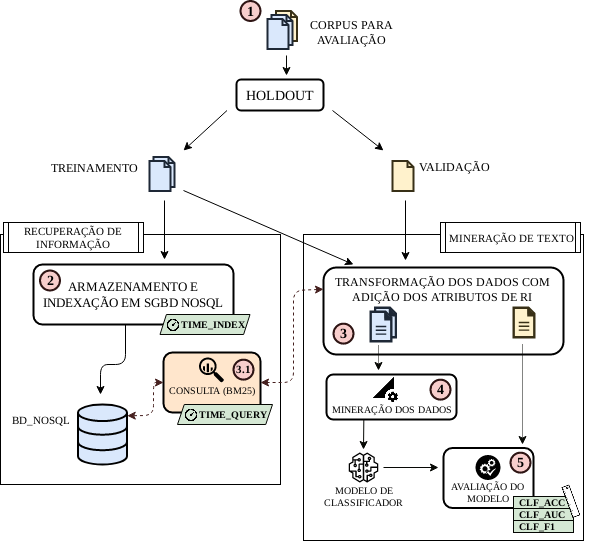
\includegraphics[width=0.8\textwidth]{img/diagrama-metodologia-v2-2.png}
    \end{center}
    \vspace{-0.5cm}
    \legend{\ABNTEXfontereduzida \textbf{Fonte:} O autor.}
    \label{fig:diagrama-da-metodologia}
\end{figure}
    
    Inicialmente é necessário selecionar os \textbf{(1) Corpus para Avaliação} que servirão para efetuar as avaliações de desempenho, e, caso esses corpus ainda não estejam segmentados em exemplos para treinamento e exemplos para validação, será feita essa separação com o método de \textit{holdout}\footnote{Particionamento aleatório do dados em dois conjuntos independentes, geralmente chamados de treinamento e teste. O conjunto de treinamento é utilizado para derivar o modelo e o de teste para estimar a sua acurácia. \cite[p.~370]{Han:2011:DMC:1972541}.} de $\frac{2}{3}$ para treinamento e $\frac{1}{3}$ para validação.
    
    Em seguida, o conjunto de treinamento passará pela fase de RI, aonde será feito o \textbf{(2) Armazenamento e Indexação em  SGBD NoSQL} por meio das ferramentas apresentadas na Seção  \ref{sec:Armazenamento-e-indexação}, sendo mensurado o tempo necessário para concluir essa operação em cada um dos Sistemas Gerenciadores de Banco de Dados (SGBD) NoSQL selecionados.
    
    O processo de Mineração de Texto pode ser segmentado em 7 etapas, conforme ressaltado anteriormente na Seção \ref{sec:MineraçãoTexto}.
    Na metodologia proposta aqui a fase de MT assume que as 3 etapas iniciais de limpeza, integração, e seleção dos dados, já foram realizadas no banco de dados de teste, assim os conjuntos divididos em treinamento e validação passarão diretamente pela etapa seguinte que é a \textbf{(3) Transformação dos dados com adição dos atributos de RI}.
    Nesta etapa, os banco de dados NoSQL indexados receberão \textbf{(3.1) Consultas} com a utilização das funções de ranqueamento baseadas no BM25 que cada ferramenta implementa, sendo mensurado o tempo para efetuar cada consulta e gerar os novos atributos sugeridos adiante na Seção \ref{sec:Atributos-de-RI-sugeridos}.
    % Será feita uma consulta para cada exemplo dos conjuntos, e a resposta dessas consultas servirá para criar os atributos de RI detalhados logo mais na Seção \ref{sec:Atributos-de-RI-sugeridos}.
    
    O processo de \textbf{(4) Mineração dos Dados} será feito por meio da réplica de soluções dos corpus para avaliação selecionados, que possuam seus códigos-fonte disponíveis, sendo então reproduzida cada solução 
    \begin{enumerate*}[label=(\alph*)]
        \item sem nenhuma alteração, e 
        \item com adição dos novos atributos sugeridos.
    \end{enumerate*}
    Esse processo gerará dois modelos de classificador, o primeiro criado sem atributos de RI e o segundo com esses atributos.
    A etapa de \textbf{(5) Avaliação do Modelo} permitirá que para cada modelo sejam geradas métricas da literatura de MT, detalhadas logo mais na Subseção \ref{subsec:Desempenho-de-classificador}, a partir do teste com o conjunto de validação, possibilitando a comparação do ganho de desempenho de classificador com/sem atributos de RI.
    % Na fase de Mineração de Texto os conjuntos de treinamento e de validação passarão pela \textbf{(3) Transformação dos dados com adição dos atributos de RI} onde 
    
    
    % Para utilização da função de ranqueamento BM25 como variável em tarefas de mineração de texto é necessário efetuar o armazenamento e a indexação dos textos do conjunto de treinamento, e para esta tarefa serão utilizadas ferramentas de armazenamento em banco de dados (não relacionais?) que fornecem implementações do BM25 para consulta, estas serão apresentadas na Seção \ref{sec:Armazenamento-e-indexação}.
    
    % Se faz necessário também definir métricas para avaliação do ganho de desempenho com as variáveis de RI, assim como elencar as bases de dados que vão servir para efetuar essa avaliação, disposto logo mais nas Seções \ref{sec:Métricas-para-avaliação-de-desempenho} e \ref{sec:Corpus-para-avaliação}.

\section{Corpus para avaliação}  \label{sec:Corpus-para-avaliação}
    Foram definidos dois corpus de competições promovidas pela PAN, sigla da organização que se originou do \textit{International Workshop on Plagiarism Analysis, Authorship Identification, and Near-Duplicate Detection} em 2007 \cite{PAN_Workshop_2007}, sendo estes descritos a seguir:% https://web.archive.org/web/20190711212207/https://www.uni-weimar.de/medien/webis/events/pan-07/pan07-web/
    
    % Os banco de dados de teste selecionados para avaliação são os utilizados na PanCLEF 2019 % necessário citar a PanCLEF anteriormente
    \begin{itemize}
    % Author Profiling - PAN @ CLEF 2018
    % Soluções disponíveis:
    % 2. daneshvar18 - https://github.com/SamanDaneshvar/pan18ap
    %  https://pan.webis.de/downloads/publications/papers/daneshvar_2018.pdf
    % 4. laporte18 - https://github.com/arthur-sultan-info/PAN2018-AP
    % https://pan.webis.de/downloads/publications/papers/ciccone_2018.pdf
    % 12. gouravdas18 - https://github.com/brajagopalcse/PAN2018
    % https://pan.webis.de/downloads/publications/papers/gopalpatra_2018.pdf
    % 16. schaetti18 - https://github.com/nschaetti/PAN18-Author-Profiling
    %  https://pan.webis.de/downloads/publications/papers/schaetti_2018a.pdf
    % 21. raiyani18 - https://github.com/kraiyani/author-profiling-pan-clef-2018 
    % https://pan.webis.de/downloads/publications/papers/raiyani_2018.pdf
    % 23. jucikarlgreen - https://github.com/jussikarlgren/pan18
    % https://pan.webis.de/downloads/publications/papers/karlgren_2018.pdf
        \item \textbf{DB\_AUTHORPROF - \textit{Author Profiling - PAN @ CLEF 2018}:} Uma tarefa da competição \textit{CLEF 2018} promovida pela PAN na classe de análise de autoria, a qual foca na identificação de gênero no Twitter em três linguagens distintas, inglês, espanhol, e árabe \cite{PAN_APCLEF_2018}.
        
        Os dados consistem de 100 \textit{tweets}\footnote{Termo utilizado para designar as publicações feitas na rede social do Twitter.} e 10 imagens para cada autor, sendo que o conjunto de treinamento possui \begin{enumerate*}[label=(\alph*)]
            \item 3000 autores em inglês, \item 3000 autores em espanhol, e \item 1500 autores em árabe,
        \end{enumerate*}
        e o conjunto de validação possui
        \begin{enumerate*}[label=(\alph*)]
            \item 1900 autores em inglês, 
            \item 2200 autores em espanhol, e 
            \item 1000 autores em árabe
        \end{enumerate*}
        \cite{rangel2018overview}.
        
        Segundo \citeonline{rangel2018overview} esse banco de dados da \textit{CLEF 2018} com um total de 12600 autores é um subconjunto da tarefa de \textit{Author Profiling} da \textit{CLEF 2017} e eles foram classificados em dois passos,
        \begin{enumerate*}[label=(\roman*)]
            \item automaticamente com a ajuda de um dicionário de nomes próprios, e
            \item manualmente verificando a foto, descrição e outros elementos de cada perfil
        \end{enumerate*}
        \cite{rangel2017overview}.
        
        % \item \textbf{DB\_BOTGENDER - \textit{Bots and Gender Profiling PAN @ CLEF 2019}:}
        % https://pan.webis.de/clef19/pan19-web/author-profiling.html
        % 7 - Ipsas & Popescu - https://github.com/adiIspas/Bots-Gender-Profiling
        % 10 - Goubin - https://github.com/pan-webis-de/goubin19
        % 11 - Polignana & de Pinto - https://github.com/pan-webis-de/polignano19
        % 23. De La Peña & Prieto - https://github.com/JoseRPrietoF/autoria
        % 30. Rahgoyu - https://github.com/HamedBabaei/PAN2019_bots_gender_profiling
        % 32 Pryzybyla Przybyła - https://github.com/pan-webis-de/przybyla19
        
        \item \textbf{DB\_HYPARTISAN - \textit{Hyperpartisan News Detection - PAN @ SemEval 2019 Task 4}:} Esta tarefa da competição \textit{SemEval 2019} promovida pela PAN consiste em, dada uma notícia, avaliar se esta segue uma argumentação hiperpartidária, que significa verificar se ela possui fidelidade cega, preconceituosa, ou irracional a um partido, grupo, causa, ou pessoa \cite{PAN_HND_2019}.
        Portanto pode-se dizer que se trata de um problema de classificação binária, a classe real é a presença ou ausência de hiperpartidarismo em cada exemplo.
        
        Os dados consistem em artigos de notícias divididos em múltiplos arquivos onde cada arquivo com parte inicial ``articles-'' consiste em uma notícia e a classificação real da notícia está presente em um arquivo com inicial ``ground-truth-''. 
        Além disso os dados estão divididos em duas partes, a primeira composta de 750 mil artigos está classificada pelo enviesamento geral do editor, onde metade está classificada como hiperpartidária e a outra metade não. 
        Dessa parte, 80\% (600 mil artigos) estão no conjunto de treinamento e 20\% (150 mil) estão no conjunto de validação, sendo que nenhum editor de artigos do conjunto de treinamento se repete no conjunto de validação \cite{johannes_kiesel_2018_1489920}.
        
        A segunda parte dos dados foi rotulada através de \textit{crowdsourcing}\footnote{Obter entrada para uma tarefa ou projeto específico contando com os serviços de um número de pessoas, pagas ou não, tipicamente através da Internet.}. 
        Essa parte dos dados contêm um total de 645 artigos, sendo estes apenas artigos para os quais existia um consenso entre os trabalhadores de crowdsourcing. 
        Destes, 238 (37\%) são hiperpartidários e 407 (63\%) não são \cite{johannes_kiesel_2018_1489920}. 
        
        % The data is split into multiple files. The articles are contained in the files with names starting with "articles-" (which validate against the XML schema article.xsd). The ground-truth information is contained in the files with names starting with "ground-truth-" (which validate against the XML schema ground-truth.xsd).
        %  https://pan.webis.de/semeval19/semeval19-web/index.html
        % https://web.archive.org/web/20190711214328/https://zenodo.org/record/1489920
    \end{itemize}
    % Descreuioes a partir da tarefa no site
    % Definir as soluçcoes disponiveis que vou utilizar (Nao pode ter RI)
    
    Os dois corpus selecionados possuem soluções de participantes nas competições da PAN que tem seu código fonte aberto e disponível em repositórios online.
    Das equipes participantes na competição do corpus DB\_AUTHORPROF, foram localizadas em repositórios de código aberto no GitHub\footnote{Plataforma de hospedagem de código-fonte com controle de versão usando o Git.} as supostas soluções  apresentadas na Tabela \ref{tab:soluções-authorprof}, ordenadas pela classificação disponível na parte de resultados da página da competição \citeonline{PAN_APCLEF_2018}.
    % Das equipes participantes na competição do corpus DB\_AUTHORPROF, foram localizadas em repositórios de código aberto no GitHub\footnote{Plataforma de hospedagem de código-fonte com controle de versão usando o Git.} as seguintes supostas soluções ordenadas pela classificação disponível na parte de resultados da página da competição \cite{PAN_APCLEF_2018}:
    % \begin{enumerate}[label=\Roman*.]
    %     \item 2. daneshvar18 - Disponível em \url{https://github.com/SamanDaneshvar/pan18ap}
        
    %     \item 4. laporte18 - Disponível em \url{https://github.com/arthur-sultan-info/PAN2018-AP}
        
    %     \item 12. gouravdas18 - Disponível em \url{https://github.com/brajagopalcse/PAN2018}
        
    %     \item 16. schaetti18 - Disponível em \url{https://github.com/nschaetti/PAN18-Author-Profiling}
        
    %     \item 21. raiyani18 - Disponível em \url{https://github.com/kraiyani/author-profiling-pan-clef-2018}
        
    %     \item 23. karlgreen18 - Disponível em \url{ https://github.com/jussikarlgren/pan18}
    % \end{enumerate}
    
    
    \begin{table}[h]
    \centering
    \caption{Soluções encontradas de participantes da competição DB\_AUTHORPROF.}
    \begin{tabular}{|c|l|l|}
        \hline
        \textbf{Posição}  
        & \makecell[l]{\textbf{Equipe}}
        & \makecell[l]{\textbf{Repositório de código no site \url{https://github.com/}}}
        \\ \hline
        2
        & daneshvar18 
        & \hyperlink{https://github.com/SamanDaneshvar/pan18ap/}{/SamanDaneshvar/pan18ap/}
        \\ \hline
        4
        & laporte18 
        & \hyperlink{https://github.com/arthur-sultan-info/PAN2018-AP/}{/arthur-sultan-info/PAN2018-AP/} 
        \\ \hline
        12
        & gouravdas18 
        & \hyperlink{https://github.com/brajagopalcse/PAN2018/}{/brajagopalcse/PAN2018/}
        \\ \hline
        16
        & schaetti18 
        & \hyperlink{https://github.com/nschaetti/PAN18-Author-Profiling}{/nschaetti/PAN18-Author-Profiling/}
        \\ \hline
        21
        & raiyani18 
        & \hyperlink{https://github.com/kraiyani/author-profiling-pan-clef-2018/}{/kraiyani/author-profiling-pan-clef-2018}
        \\ \hline
        23
        & karlgreen18 
        & \hyperlink{https://github.com/jussikarlgren/pan18}{/jussikarlgren/pan18/}
        \\ \hline
    \end{tabular}
    \legend{\ABNTEXfontereduzida \textbf{Fonte:} Classificações obtidas de \citeonline{PAN_APCLEF_2018}, e repositórios encontrados pelo autor.}
    \label{tab:soluções-authorprof}
\end{table}
    
    % Quanto à competição referente ao corpus DB\_HYPARTISAN foram encontrados os seguintes repositórios disponíveis na ordem de classificação da página da competição \cite{PAN_HND_2019}:
    % \begin{enumerate}[label=\Roman*.]
    %     \item 1. bertha-von-suttner - Disponível em \url{https://github.com/GateNLP/semeval2019-hyperpartisan-bertha-von-suttner/}
        
    %     \item 4. tom-jumbo-grumbo - Disponível em \url{https://github.com/chialun-yeh/SemEval2019/}
        
    %     \item 10. clint-buchanan - Disponível em \url{https://github.com/hmc-cs159-fall2018/final-project-team-mvp-10000/}
        
    %     \item 13. paparazzo - Disponível em \url{https://github.com/ngannlt/semeval2019-hyperpartisan-paparazzo/}
        
    %     \item 17. spider-jerusalem - Disponível em \url{https://github.com/amal994/hyperpartisan-detection-task/}
        
    %     \item 19. doris-martin - Disponível em \url{https://github.com/ixa-ehu/ixa-pipe-doc/}
    % \end{enumerate}
    Quanto à competição referente ao corpus DB\_HYPARTISAN foram encontrados os repositórios disponíveis na ordem de classificação da página da competição \cite{PAN_HND_2019}, dispostos abaixo na Tabela \ref{tab:soluções-hyperpartisan}.
    
    \begin{table}[ht]
    \centering
    \caption{Soluções encontradas de participantes da competição DB\_HYPERPARTISAN.}
    \begin{adjustbox}{max width={\textwidth},keepaspectratio}%
    \begin{tabular}{|c|l|l|}
        \hline
        \textbf{Posição}  
        & \makecell[l]{\textbf{Equipe}}
        & \makecell[l]{\textbf{Repositório de código no site \url{https://github.com/}}}
        \\ \hline
        1
        & bertha-von-suttner 
        & \hyperlink{https://github.com/GateNLP/semeval2019-hyperpartisan-bertha-von-suttner/}{/GateNLP/semeval2019-hyperpartisan-bertha-von-suttner/}
        \\ \hline
        4
        & tom-jumbo-grumbo 
        & \hyperlink{https://github.com/chialun-yeh/SemEval2019/}{/chialun-yeh/SemEval2019/} 
        \\ \hline
        10
        & clint-buchanan 
        & \hyperlink{https://github.com/hmc-cs159-fall2018/final-project-team-mvp-10000/}{/hmc-cs159-fall2018/final-project-team-mvp-10000/}
        \\ \hline
        13
        & paparazzo 
        & \hyperlink{https://github.com/ngannlt/semeval2019-hyperpartisan-paparazzo/}{/ngannlt/semeval2019-hyperpartisan-paparazzo/}
        \\ \hline
        17
        & spider-jerusalem 
        & \hyperlink{https://github.com/amal994/hyperpartisan-detection-task/}{/amal994/hyperpartisan-detection-task/}
        \\ \hline
        19
        & doris-martin 
        & \hyperlink{https://github.com/ixa-ehu/ixa-pipe-doc/}{/ixa-ehu/ixa-pipe-doc/}
        \\ \hline
    \end{tabular}
    \end{adjustbox}
    \legend{\ABNTEXfontereduzida \textbf{Fonte:} \cite{PAN_HNDLEADERBOARD_2019}.}
    \label{tab:soluções-hyperpartisan}
\end{table}

    As soluções com código fonte encontradas serão analisadas para garantir que já não façam uso da criação de atributos baseados em RI.
    Então, no mínimo uma solução de cada BD será executada para verificação das pontuações obtidas na competição e obtenção das métricas de desempenho de classificador (ver a Subseção \ref{subsec:Desempenho-de-classificador}).
    Em seguida, será executado o processo completo da metodologia apresentada na Figura \ref{fig:diagrama-da-metodologia}, para mensurar o desempenho computacional das ferramentas de armazenamento e indexação, e o desempenho do classificador com os atributos de RI.
    
    
\section{Armazenamento e indexação} \label{sec:Armazenamento-e-indexação}

    Para armazenar e indexar os corpus das tarefas de Mineração de Textos em bancos de dados, possibilitando o cálculo da função BM25 para que sejam gerados os atributos sugeridos na Seção \ref{sec:Atributos-de-RI-sugeridos} para cada exemplo, serão utilizadas as seguintes tecnologias que fazem implementações do BM25:
    \begin{itemize}
        \item \textbf{TOOL\_ELASTIC}: Elasticsearch 7.2 é o mecanismo distribuído de análise e busca baseado no Apache Lucene\footnote{Biblioteca de software livre e de código aberto para ferramentas de buscas em texto, escrita originalmente em Java \cite{LUCENE_DOCUMENTATION_2019}.}, desenvolvido em Java, e possui código aberto sob diversas licenças sendo a principal a Licença Apache\footnote{Licença de software livre permissiva de autoria da Apache Software Foundation (ASF) \cite{NEWMEDIA_OPENGUIDE_2015}.} \cite{ELASTIC_GitHub_2019, ELASTIC_REFERENCE_INTRO_2019}.  % https://www.elastic.co/guide/en/elasticsearch/reference/current/index-modules-similarity.html
        % https://www.elastic.co/pt/blog/practical-bm25-part-2-the-bm25-algorithm-and-its-variables
        
        O Elasticsearch possui diversas APIs que possibilitam sua integração fácil com variadas linguagens de programação \cite{ELASTIC_GitHub_2019}, e tenta deixar todas suas funcionalidades disponíveis via sua API JSON pois internamente é no formato JSON\footnote{\textit{JavaScript Object Notation}, formato de objeto utilizado pela linguagem de programação JavaScript.} que o Elasticsearch guarda os dados. 
        Suporta também requisições GET em tempo real, o que o torna apropriado para armazenamento como um banco de dados NoSQL \cite{PETER_ELASTICDB_2011, VOLKAN_ELASTIC_DATASTORE_2018}.
        
        Dentre suas funções de indexação, o Elasticsearch possui um módulo de similaridade (\textit{similarity module}) que é responsável pela implantação de funções para ranqueamento de documentos.
        Este módulo realiza uma implementação da função BM25 como sua função padrão para cálculo de similaridade sobre o nome de \textit{BM25 similarity} \cite{ELASTIC_REFERENCE_SIMILARITY_2019}.
        
        \item \textbf{TOOL\_ARANGO}: ArangoDB v3.4.6 é um banco de dados multi-modelo nativo, desenvolvido principalmente em C++ com extensões em JavaScript, que possui código-fonte aberto e possibilita modelos de dados flexíveis, tanto para documentos, gráficos, e valores-chave \cite{ARANGODB_DOC_2019, ARANGODB_GitHub_2019}.
        % https://www.arangodb.com/docs/stable/aql/views-arango-search.html#bm25
        % https://www.arangodb.com/news/introducing-arangodb-3-4/
        
        Utiliza da linguagem de consulta AQL (\textit{ArangoDB Query Language}) para recuperar e modificar dados, que, por meio das \textit{views}\footnote{EXPLICAR O QUE É UMA VIEW DE BANCO DE DADOS.} do tipo arangosearch, introduz uma camada de integração com a biblioteca IResearch\footnote{Biblioteca de mecanismo de busca orientada a documentos, multiplataforma, e de alto desempenho, escrita inteiramente em C++, com o foco em uma conectividade de diferentes modelos de ranqueamento/similaridade \cite{IRESEARCH_GITHUB_2019}.}.
        Assim, por meio da AQL integrada ao IResearch, o ArangoDB fornece funções de ordenação de documentos mediante uma consulta, e, dentre elas, a função BM25() faz uma implementação do algoritmo da função de ranqueamento BM25 \cite{ARANGODB_SEARCHVIEWS_2019}.
        
        \item \textbf{TOOL\_ZETTAIR}: Zettair v0.9.3 é um mecanismo de busca de código-fonte aberto escrito na linguagem C, projetado para ser compacto e pesquisar rapidamente em texto, desenvolvido pelo Grupo de Mecanismos de Busca do Instituto Real de Tecnologia de Melbourne em 2009 \cite{ZETTAIR_HOME_2009}.
        % http://www.seg.rmit.edu.au/zettair/doc/Readme.html
        O Zettair permite que coleções no formato HTML ou TREC sejam indexadas para busca, e possui como característica principal a habilidade de lidar com grandes quantidades de texto, ele constrói índices invertidos por meio da análise feita no seu modo de construção de índex \cite{ZETTAIR_INDEX_2009}.
        
        Os arquivos de índices invertidos construídos pelo Zettair podem então ser consultados utilizando duas métricas diferentes \cite{ZETTAIR_USAGE_2009}:
        \begin{itemize}
            \item \textbf{--cosine}: Uma implementação da métrica da similaridade do cosseno vista na Subsubseção \ref{subsubsec:Modelo-espaço-vetorial}; e
            
            \item \textbf{--okapi}: Implementação da função BM25, também chamada de Okapi BM25, como apresentada na Subsubseção \ref{subsubsec:Modelo-probabilístico}.
        \end{itemize}
        
        % \item Apache Spark
        % COmentado pois o Spark não implementa o BM25.
    \end{itemize}
    % Links dos sites das ferramentas como notas de rodapé.
    % Citar a versão de cada ferramenta que vai ser utilizada.
    % 
    

 
% Metodologia:

% Vão ser elencadas as tecnologias para armazenamento e indexação dos dados por meio do BM25:
% * Elasticsearch
% * APache Spark
% * ArangoDB
% * Zettair

% Os bancos de teste serão:
% * PanCLEF Hyperpartisan 2019
% https://pan.webis.de/semeval19/semeval19-web/leaderboard.html
% * A definir
% * Bots and Gender Profilin % PAN @ CLEF 2019 

\section{Atributos de RI sugeridos}  \label{sec:Atributos-de-RI-sugeridos}
    Os atributos baseados em Recuperação de Informação sugeridos para a presente pesquisa são fundamentados na investigação de \citeonline{WEREN_MESTRADO_2014}, derivada de seus trabalhos anteriores \cite{WEREN_CLEF_2014,WEREN_ARTIGO_2014}, os quais mostram resultados positivos da utilização de atributos derivados de RI numa tarefa de Mineração de Texto.
    Nesses trabalhos, para identificação de perfis de autoria, são utilizados grupos de atributos derivados de RI, os quais representam a seguinte hipótese: os autores de um mesmo grupo de gênero ou idade tendem a usar termos semelhantes, e que a distribuição desses termos difere entre os grupos \cite[p.~20]{WEREN_MESTRADO_2014}.
    
    Esse mesmo pressuposto, da investigação feita por \citeonline{WEREN_MESTRADO_2014}, é assumido aqui, sendo generalizado para outras classes de identificação de autoria, como por exemplo que autores de artigos hiperpartidários tendem a usar termos semelhantes, e a distribuição desses termos difere de autores não hiperpartidários.
    
    Cada exemplo do corpus a ser classificado será usado como consulta ao banco de dados NoSQL indexado, e cada uma destas consultas terá como resultado uma lista dos \textit{top-$k$} exemplos presentes no banco de dados, ordenada por pontuação de similaridade da função BM25, sendo esta pontuação calculada pela ferramenta de armazenamento indexação. Este procedimento está representado na Figura \ref{fig:diagrama-cosulta-geração-atributos}.
    
    \begin{figure}[H]
    \centering
    \caption{Metodologia de consulta aos BD para geração dos atributos sugeridos.}
    \begin{center}
        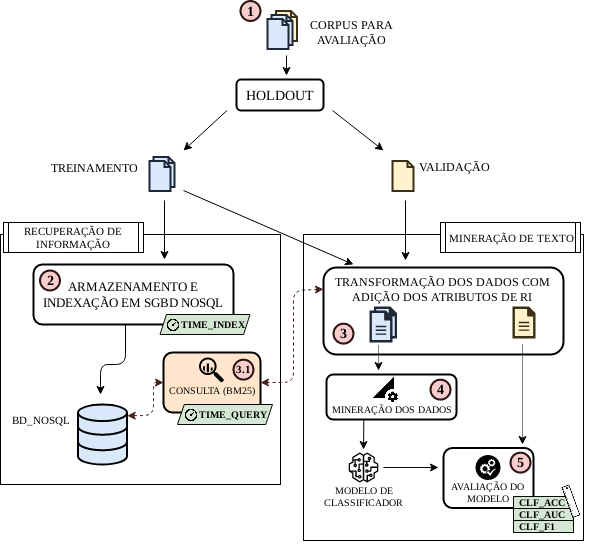
\includegraphics[width=0.8\textwidth]{img/diagrama-metodologia-v2-1.png}
    \end{center}
    \vspace{-0.5cm}
    \legend{\ABNTEXfontereduzida \textbf{Fonte:} O autor.}
    \label{fig:diagrama-cosulta-geração-atributos}
\end{figure}
    
    O cálculo dos novos atributos será feito a partir da lista retornada dos \textit{top-$k$} exemplos, onde serão utilizadas as três funções de agregação sugeridas por \citeonline[p.~21--23]{WEREN_MESTRADO_2014}:
    \begin{enumerate*}[label=(\alph*)]
        \item média,
        \item soma, e
        \item contagem
    \end{enumerate*}, 
    levando em conta a classe binária da tarefa de classificação. 
    Assim, serão gerados os atributos apresentados na Tabela \ref{tab:lista-atributos-sugeridos}.
    
    \begin{table}[H]
    \centering
    \begin{tabular}{|p{4.0cm}|l|l|}
        \hline
        \diagbox[width=4.4cm, height=2.0cm]{Agregação}{
            \raisebox{-1.3cm}{
                \rotatebox{90}{
                    \parbox{1.2cm}{\centering Exemplo}
                }
            }
        }  
        & \makecell[l]{Não faz parte da \\ classe da tarefa}
        & \makecell[l]{Faz parte da \\ classe da tarefa}
        \\ \hline
        \makecell[l]{Média aritmética \\ das pontuações}
        & \textbf{CLASS\_0\_BM25\_AVG} 
        & \textbf{CLASS\_1\_BM25\_AVG}  
        \\ \hline
        \makecell[l]{Contagem do número \\ de resultados}
        & \textbf{CLASS\_0\_BM25\_COUNT} 
        & \textbf{CLASS\_1\_BM25\_COUNT}  
        \\ \hline
        \makecell[l]{Soma das \\ pontuações}
        & \textbf{CLASS\_0\_BM25\_SUM} 
        & \textbf{CLASS\_1\_BM25\_SUM}  
        \\ 
        \hline
    \end{tabular}
    \caption{Atributos derivados de RI sugeridos.}
    \label{tab:lista-atributos-sugeridos}
\end{table}
    % Assim, serão geradas os seguintes atributos:
    % \begin{itemize}
    %     \item \textbf{CLASS\_0\_BM25\_AVG:} Média aritmética das pontuações dos resultados retornados pela consulta, que não fazem parte da classe da tarefa.
    %     \item \textbf{CLASS\_0\_BM25\_COUNT:} Contagem do número de resultados retornados pela consulta, que não fazem parte da classe da tarefa.
    %     \item \textbf{CLASS\_0\_BM25\_SUM:} Soma das pontuações dos resultados retornados pela consulta, que não fazem parte da classe da tarefa.        
    %     \item \textbf{CLASS\_1\_BM25\_AVG:} Média aritmética das pontuações dos resultados retornados pela consulta, que fazem parte da classe da tarefa.
    %     \item \textbf{CLASS\_1\_BM25\_COUNT:} Contagem do número de resultados retornados pela consulta, que fazem parte da classe da tarefa.
    %     \item \textbf{CLASS\_1\_BM25\_SUM:} Soma das pontuações dos resultados retornados pela consulta, que fazem parte da classe da tarefa.
    % \end{itemize}
    
    
    
%  Por exemplo, para a classificação binária do PANCLEF 2019 Hyperpartisan podem ser criadas as variáveis a seguir:
% * avg_0 
% * count_0
% * sum_0
% * avg_1
% * count_1
% * sum_1

% baseadas no weren (2014)


\section{Métricas para avaliação de desempenho}  \label{sec:Métricas-para-avaliação-de-desempenho}
    Serão avaliados
    \begin{enumerate*}[label=(\alph*)]
        \item o desempenho das ferramentas utilizadas para indexação e consulta, por meio da avaliação temporal do desempenho computacional, e também
        \item o ganho de desempenho propiciado pelo uso das variáveis de RI em termos das métricas de classificadores de Mineração de Texto. % Essas métricas tem que ser citadas no referencial teórico.
    \end{enumerate*} 
    
    \subsection{Desempenho computacional das ferramentas}  \label{subsec:Desempenho-computacional}
        Para avaliar o desempenho das ferramentas de armazenamento e indexação serão utilizadas duas métricas temporais:
        \begin{itemize}
            \item \textbf{TIME\_INDEX}: Tempo de execução para indexar o conjunto de treinamento de cada um dos banco de dados de teste elencados na Seção \ref{sec:Corpus-para-avaliação}. Dadas as quatro diferentes ferramentas de indexação e os dois banco de dados selecionados, serão computadas 8 TIME\_INDEX para comparação;
            
            \item \textbf{TIME\_QUERY}: Tempo para consulta de cada exemplo do conjunto de teste e geração das variáveis sugeridas na Seção \ref{sec:Atributos-de-RI-sugeridos} para o item específico. Dadas as 12 variáveis sugeridas para criação distribuídas nos dois banco de dados selecionados, e dadas as 4 ferramentas de indexação, 48 TIME\_QUERY serão computadas.  
        \end{itemize}
        
        Essas variáveis serão computadas para cada uma das 4 ferramentas selecionadas sendo executadas no mesmo sistema computacional a fim de oferecer maior confiança aos números obtidos. 
        O sistema computacional a ser utilizado para efetuar o experimento ainda não está definido, mas será especificado nos resultados.
    
% O teste de desempenho será feito comparando as ferramentas de indexação, tempo para indexar o treino de cada banco (TIME_TRN) em cada ferramenta.

% O tempo para consultar para cada linha do teste as variáveis a serem criadas (no caso de classificação binária iremos definir agregações do tipo count, sum e avg). Por exemplo, para a classificação binária do PANCLEF 2019 Hyperpartisan podem ser criadas as variáveis a seguir:
% * avg_0 
% * count_0
% * sum_0
% * avg_1
% * count_1
% * sum_1
    \subsection{Desempenho de classificador}  \label{subsec:Desempenho-de-classificador}
    O ganho de desempenho propiciado pelos atributos de RI criados será mensurado por métricas de desempenho de classificadores da literatura de Mineração de Dados, as mesmas da Mineração de Texto.
    Nesse estudo serão computadas as seguintes métricas:
    \begin{itemize}
        \item \textbf{CLF\_ACC}: Acurácia do classificador no conjunto de validação.
        \item \textbf{CLF\_AUC}: Área sob a curva ROC.

        % Comentadas pois Rosalvo disse para ficar somente com acurácia (utilizada nas competições) e a área sob a curva ROC.
        % \item \textbf{CLF\_F1}: F1-Score
        % \item \textbf{CLF\_PRE}: Precisão do classificador.
        % \item \textbf{CLF\_REC}: Revocação do classificador.
    \end{itemize}
    A acurácia de um classificador é a razão entre o número de exemplos classificados corretamente, e o número total de exemplos, no caso em questão, a variável \textbf{CLF\_ACC} a ser computada é referente ao conjunto de validação.
    
% Ao final será comparado o ganho de desempenho (acurácia, precisão, recall e F1-score) nas melhores soluções dos bancos definidos a partir da adição das variáveis criadas.
% Por exemplo para a PANCLEF 2019 Hyperpartisan será utilizada a solução que está disponível no github com melhor score e ela será executada novamente para conferir o resultado obtido de acurária que eles dizem e então será rodado novamente com a adição das variáveis de RI (BM25).

% \subsection{Subseção de exemplo 1 - Referenciando seções} \label{subsec:subsec1}






%--------------------------------------------------------------------------------------
% Insere a seção de cronograma
% Está comentada porque só é necessária no TCC I
%--------------------------------------------------------------------------------------
%--------------------------------------------------------------------------------------
% Insere a seção de cronograma
%--------------------------------------------------------------------------------------

\section{Cronograma} \label{sec:Cronograma}

A Tabela \ref{tab:cronograma} mostra o cronograma de atividades a serem executadas para o Trabalho de Conclusão II (TCC II), com base no calendário do período 2019.2 da UNIVASF, definido pelo Calendário Acadêmico 2019 da instituição.

\begin{table}[!thb]
	%\huge
    \centering
    \caption{Cronograma das atividades previstas para o TCC II.}
    \begin{adjustbox}{max width=\textwidth}
    \begin{tabular}{p{6.5cm}|c|c|c|c|c|c}
        \toprule
        \textbf{Atividade}
        & Set & Out & Nov & Dez & Jan & Fev
        \\ \hline
        Definição e obtenção dos corpus para avaliação 
        & X   &     &     &     &     &          
        \\ \hline
        Inspeção e seleção das soluções com código fonte disponível
        & X   &     &     &     &     &          
        \\ \hline
        Instalação e familiarização com as ferramentas de arquivamento e indexação
        & X   & X   &     &     &     &          
        \\ \hline
        Indexação do conjunto de treinamento dos corpus
        &     & X   & X   &     &     &          
        \\ \hline
        Adição dos atributos de RI às soluções selecionadas
        &     & X   & X   &     &     &    
        \\ \hline
        Mineração dos dados por meio da reprodução das soluções selecionadas com/sem adição dos atributos de RI
        &     &     & X   & X   & X   &  
        \\ \hline
        Escrita do TCC II                       
        & X   & X   & X   & X   & X   &         
        \\ \hline
        Defesa do TCC II                        
        &     &     &     &     & X   &        
        \\
        \bottomrule
    \end{tabular}
    \end{adjustbox}
    
    \label{tab:cronograma} 
    % \legend{\textbf{Fonte:} O autor.}
\end{table}

		\chapter{Resultados} \label{ch:Resultados}
	%  Os resultados seguem a metodologia

	% Definir qual o top_k utilizado
	% Verificar em Were2014 novamente
	% Padrão do zettair (se não me engano é 20)
	% Artigo de fulano não diz

	% Capítulo de Resultados 

	% -> Introdução: "Este capítulo apresenta os resultados obtidos e discute-os..." 
	Este capítulo apresenta os resultados obtidos neste estudo investigativo do desempenho de atributos de RI em classificadores de Mineração de Texto.

	Nas subseções a seguir primeiro é abordada a configuração experimental utilizada para realizar o estudo, e logo em seguida é apresentada uma visão geral das soluções selecionadas dos corpus DB\_AUTHORPROF e DB\_HYPERPARTISAN, na qual o pré-processamento realizado e os classificadores utilizados em cada uma das soluções são descritos brevemente.
	Por fim, são apresentados os resultados mensurados por meio das medidas escolhidas para avaliação de desempenho, na Seção \ref{sec:DesempenhoFerramentas} estão as medidas de desempenho das ferramentas de armazenamento e indexação, e na Seção \ref{sec:DesempenhoClassificadores} são expostas as medidas de desempenho dos classificadores.

	% Na subseção a seguir são abordados os resultados referentes às ferramentas de indexação.
	% Na subseção posterior são abordados os resultados referente aos desempenho das variáveis de RI em classificadores.

	\section{Configuração experimental} \label{sec:ConfiguraçãoExperimental}
	% 4.0 Setup experimental 

		Para programação e execução dos experimentos foi utilizado o sistema computacional disponível para o autor, com a configuração disposta na Tabela \ref{tab:sistema-computacional}.

		\begin{table}[ht]
    \centering
    \caption{Configuração do computador de mesa utilizado neste estudo.}
    \begin{adjustbox}{max width={\textwidth},keepaspectratio}%
    \begin{tabular}{|l|l|}
        \hline
        % \textbf{Posição}  
        % & \makecell[l]{\textbf{Equipe}}
        % & \makecell[l]{\textbf{Repositório de código no site \url{https://github.com/}}}
        % \\ \hline
        Processador
        & Intel(R) Core(TM) i7-4770 CPU @ 3.40GHz
        \\ \hline
        Memória RAM
        & 32370 MB
        \\ \hline
        Sistema Operacional
        & Linux Mint 19.2 Tina
        \\ \hline
        Placa-mãe
        & Gigabyte Z97-D3H
        \\ \hline
        Gráficos
        & Mesa DRI Intel(R) Haswell Desktop
        \\ \hline
        Disco
        & HP SSD EX920 512GB
        \\ \hline
    \end{tabular}
    \end{adjustbox}
    \legend{\ABNTEXfontereduzida \textbf{Fonte:} O autor.}
    \label{tab:sistema-computacional}
\end{table}
		
		As ferramentas de armazenamento e indexação receberam os mesmos parâmetros de refinamento na configuração de suas funções BM25, sendo estes configurados em $k_1 = 1.2$, $k_3 = 0$ e $b = 0.75$.
		O parâmetro $k_3$ (escalonar frequência de termos na consulta) é exclusivo do Zettair, as demais ferramentas não implementam este parâmetro.

		% Fixação do número aleatório do Python e das bibliotecas utilizadas nas soluções, quando isto não era feito originalmente, para permitir reprodutibilidade exata dos resultados obtidos.
		% [ ] FOOTNOTE DO VSCODIUM?
		O ambiente de programação utilizado foi o VSCodium e a linguagem de programação utilizada foi o Python 3.7.5.
		Para permitir reprodutibilidade dos resultados obtidos, o gerador de números aleatórios (RNG) do ambiente do Python, assim como os RNGs das bibliotecas utilizadas pelas soluções, tiveram as suas sementes de geração fixadas.

		Todos os códigos fontes dos scripts Python criados para este estudo estão disponíveis em um repositório de código online e público criado pelo autor, acessível pelo seguinte link: \hyperlink{https://github.com/ruanmed/tcc-ii-ir-features-text-mining/}{https://github.com/ruanmed/tcc-ii-ir-features-text-mining/}.
		A seguir são tratadas as dependências de \textit{software} para execução do estudo.

		\subsection{Dependências de \textit{software}} \label{subsec:DependênciasSoftware}
			Para execução dos scripts Python gerados por esse estudo é necessário Python >= 3.6 com as bibliotecas elasticsearch-py >= 7.0.5 e python-arango >= 5.2.1.
			Ambas bibliotecas se encontram disponíveis no PyPI (\textit{Python Package Index}, ou índice de pacotes do Python em tradução livre).

			Também é necessário possuir instâncias do Elasticsearch >= 7.4.0 e do ArangoDB >= 3.5.1 rodando e disponíveis na rede local do sistema, isso pode ser feito por meio da instalação dessas ferramentas no sistema local.
			O Zettair >= 0.94 também é necessário estar instalado no sistema, sendo possível executá-lo pelo terminal de comandos com o comando 'zet'.

			A instalação das três ferramentas em sistemas Linux foi simplificada com a criação de um arquivo Docker que utiliza de imagens disponíveis online do ArangoDB e do Elasticsearch, reduzindo o número de comandos necessários para executar as ferramentas no sistema computacional.
			Detalhes de como utilizar esse arquivo Docker se encontram em: \hyperlink{https://github.com/ruanmed/tcc-ii-ir-features-text-mining\#docker-file}{https://github.com/ruanmed/tcc-ii-ir-features-text-mining\#docker-file}.

			Além dessas dependências, é necessário também instalar as bibliotecas específicas de cada uma das soluções selecionadas.
			Essas estão listadas nos arquivos README disponibilizados junto às soluções.

	\section{Visão geral das soluções selecionadas e adaptações feitas} \label{sec:VisãoSoluçõesEAdaptações}
		% Falar brevemento sobre o pré-processamento;
		% Falar sobre o classificador utilizado; e
		% Indicar o Notebook de cada solução para mais detalhes
		As soluções selecionadas para reprodução e posterior adição dos atributos de RI utilizam de diferentes técnicas para pré-processamento dos corpus e também de classificadores diferentes, tornando necessário, em alguns casos, ajustes antes da adição dos atributos de RI.

		Nas subseções a seguir são brevemente abordadas as soluções 1\_bertha e 4\_tom do corpus DB\_HYPARTISAN, e a solução 2\_daneshvar18 do corpus DB\_AUTHORPROF.

		\subsection{Corpus DB\_HYPERPARTISAN}
			O corpus DB\_HYPERPARTISAN possui dois conjuntos de dados, o primeiro com 750 mil artigos classificados por enviesamento do editor, e o segundo com 645 artigos rotulados como hiperpartidários ou não com consenso entre avaliadores via \textit{crowdsourcing}.
			O objetivo da competição que utilizou esse corpus era classificar artigos como hiperpartidários ou não, e assim os participantes puderam utilizar os dois conjuntos para fazer suas avaliações. 
			No entanto, a utilização dos 750 mil artigos classificados por enviesamento de editor não foram úteis para ajudar na classificação, e das duas soluções selecionadas nenhuma delas utilizou esses 750 mil artigos nos seus modelos finais, pois utilizar a informação de editor em conjunto reduziu o desempenho de seus classificadores \cite[p.~840]{jiang-etal-2019-team} pois segundo \citeonline[p.~1067]{yeh-etal-2019-tom} o conjunto de dados classificado por enviesamento do editor possui muito ruído.
			% Nota de rodapé sobre ruído

			O conjunto de validação final da competição, com 628 artigos também classificados manualmente, não foi disponibilizado ao público, portanto para reprodução das soluções foi necessário dividir o conjunto de 645 artigos em treinamento e validação pelo método de \textit{holdout}, ficando assim com 430 artigos para treinamento e 215 artigos para teste. 
			Essa divisão foi feita de modo que as classes mantiveram-se com o mesmo balanceamento do conjunto original (37\% dos artigos hiperpartidário e 63\% não hiperpartidários).

			Então, os 430 artigos foram indexados em todas as ferramentas de indexação permitindo a posterior geração dos atributos de RI.
			A indexação foi feita com auxílio da classe \textit{IndexToolManager} criada pelo autor, que é abordada com detalhes na seção de desempenho das ferramentas de armazenamento e indexação.
			
			\subsubsection{Solução 1\_bertha}
				A solução da equipe Bertha von Suttner (4\_bertha) para essa tarefa da \textit{SemEval 2019} consiste em uma abordagem de classificação com uma Rede Neural Convolucional (\textit{Convolutional Neural Network}, CNN) e o pré-processamento dos documentos do corpus em uma representação destes por meio de uma Rede ESRC (\textit{ELMo Sentence Representation Convolutional Network}), uma representação sugerida e nomeada pela equipe.

				A representação na Rede ESRC é uma alternativa à representação usual dos documentos por termos (ou \textit{tokens}).
				Essa representação consiste no cálculo da média dos agregados ELMo para os documentos, a nível de frase, e cada documento é representado como uma sequência desses agregados, que são vetores de tamanho de 1024 \textit{floats}. 
				Na implementação da solução cada documento é limitado a ocupar até 200 vetores de tamanho 1024, sendo então cada documento padronizado com forma 200 x 1024.
				ELMo é uma representação de palavras com contextualização profunda, que modela características complexas de uso das palavras, como sintaxe e semântica, e o uso dessas palavras em contextos linguísticos \cite{ELMoDBLP:journals/corr/abs-1802-05365}.

				A CNN do classificador consiste de 5 camadas convolucionais paralelas internamente que recebem como entrada os agregados ELMo, essas 5 camadas convolucionais se conectam a camada de saída da rede neural, com função de ativação sigmoid, mais detalhes da implementação da CNN podem ser vistos em \citeonline{jiang-etal-2019-team}.

				Para adicionar os 6 atributos de RI à rede foram embutidos, ao final de cada representação de documento, 6 vetores de tamanho 1024, preenchidos pelo valor calculado de cada atributo para o respectivo documento, resultando em documentos com forma 206 x 1024.
				A adaptação da solução está ilustrada na Figura \ref{fig:1-bertha-arquitetura-com-ri}.
				
				\begin{figure}[ht]
    \centering
    \caption{Arquitetura de sistema da solução 1\underscore{}bertha após adaptação.}
    \begin{center}
        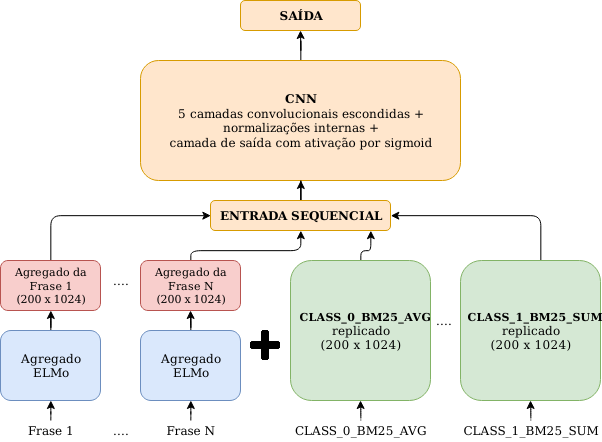
\includegraphics[width=0.75\textwidth]{img/1-bertha-arquitetura-com-ri.png}
    \end{center}
    \vspace{-0.5cm}
    \legend{\ABNTEXfontereduzida \textbf{Fonte:} O autor.}
    \label{fig:1-bertha-arquitetura-com-ri}
\end{figure}

				% \ref{fig:1-bertha-arquitetura-com-ri}
				A Figura \ref{fig:1-bertha-arquitetura-com-ri} é baseada na figura de representação de arquitetura do sistema apresentada no artigo de descrição da solução da equipe \cite{jiang-etal-2019-team}, alguns detalhes da CNN são abstraídos e os atributos de RI adicionados estão representados em verde.

				% Tem que adicionar aqui sobre o modo que a solução faz a predição

			\subsubsection{Solução 4\_tom}
				A solução da equipe Tom Jumbo-Grumbo (4\_tom) utilizou de dois classificadores, um de Regressão Logística e outro de Máquinas de Vetor de Suporte (SVMs), sendo o utilizado no modelo final o classificador SVC (C-Support Vector Classification) da biblioteca sklearn para Python.
				Uma SVM funciona transformando os dados de treinamento para uma dimensão maior e então executa uma busca pelo melhor limite de decisão, chamado de hiperplano, para separar as classes \cite[p.~408]{Han:2011:DMC:1972541}.
				Em especial, o classificador SVC da biblioteca sklearn possui um parâmetro de regularização de sua função de custo (parâmetro chamado de C) que deve ser estritamente positivo, o valor padrão é definido como $C = 1,0$, no entanto a solução da equipe, conforme disposto no código fonte disponível online, utilizou $C = 0,9$ após uma análise com diferentes valores.

				No pré-processamento, a equipe utilizou três estratégias para converter os documentos em atributos para o classificador.
				A primeira foi de criar vetores baseados na frequência dos termos, descartando termos que apareçam em mais de 90\% dos documentos e utilizando os 50 mil termos mais frequentes dos que sobrarem, guardando o valor tf-idf para cada termo respectivo ao documento.
				A segunda foi treinar um modelo PV-DM para gerar os atributos referentes a cada documento.
				E a terceira utilizou um agregado pré-treinado em textos da Wikipédia com o algoritmo GloVe, que, similarmente aos agregados ELMo, tentam também inferir o significado das palavras dos documentos.

				A arquitetura com melhor resultado foi a utilização dos atributos GloVe com o classificador SVM da biblioteca sklearn.
				Os documentos são convertidos para os vetores GloVe pré-treinados a partir se suas primeiras 1000 palavras, esses vetores GloVe possuem 300 dimensões por palavra, o que resultaria numa representação com forma de 1000 x 300, no entanto o vetor final que representa cada documento é a média dos vetores de palavras respectivo.

				\begin{figure}[h]
    \centering
    \caption{Arquitetura de sistema da solução 4\_tom após adaptação.}
    \begin{center}
        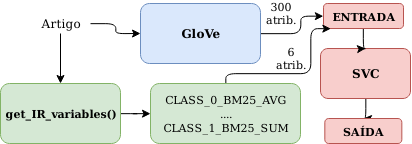
\includegraphics[width=0.68\textwidth]{img/4-tom-arquitetura-com-ri.png}
    \end{center}
    \vspace{-0.5cm}
    \legend{\ABNTEXfontereduzida \textbf{Fonte:} O autor.}
    \label{fig:4-tom-arquitetura-com-ri}
\end{figure}

				Para adicionar os 6 atributos de RI estes foram calculados para os respectivos documentos e embutidos no vetor GloVe do documento, resultando em documentos representados por 306 dimensões, ou 306 atributos.
				A arquitetura da solução adaptada está ilustrada na Figura \ref{fig:4-tom-arquitetura-com-ri}.
				% \ref{fig:4-tom-arquitetura-com-ri}

		\subsection{Corpus DB\_AUTHORPROF}
			O corpus DB\_AUTHORPROF consiste de \textit{tweets} de autores em três línguas diferentes, inglês, espanhol e árabe.
			Para avaliação dos atributos de RI o escopo de melhoria de desempenho foram considerados somente os classificadores das soluções para os autores de língua inglesa, e as imagens não foram consideradas.

			O conjunto de treinamento de autores da língua inglesa consiste de 300 mil \textit{tweets} de 3000 autores diferentes, e como o conjunto de validação final está disponível ao público, necessário somente solicitar o acesso, não foi necessário fazer o \textit{holdout} do conjunto de treinamento.
			O conjunto de validação da língua inglesa consiste de 190 mil tweets de 1900 autores.

			Os 300 mil \textit{tweets} foram indexados em todas as ferramentas de indexação permitindo a geração dos atributos de RI posteriormente para cada \textit{tweet} específico.

			\subsubsection{Solução 2\_daneshvar18}
			% baseou o seu pré-processamento em soluções das melhores equipes dos anos anteriores em tarefas da PAN CLEF
			%  O QUE É N-GRAM
				A solução de \citeonline{daneshvar:2018} utilizou um classificador SVM com diferentes tipos de $n$-grams de palavras e caracteres como atributos, e o melhor resultado obtido foi com a criação dos $n$-grams, posterior redução de dimensionalidade e então utilização do classificador LinearSVC da biblioteca sklearn para Python para criar o modelo de classificação.

				A adaptação da solução para adicionar os atributos de RI poderia ser feita adicionando os atributos antes ou depois da redução de dimensionalidade utilizada pela equipe.
				Os documentos inicialmente são representados por vetores de 1243271 dimensões, após a diminuição da dimensionalidade cada documento é representado por um vetor de 300 dimensões.
				No entanto, uma peculiaridade da solução está em como é feita a classificação, os 100 \textit{tweets} de cada autor são tratados como um único documento, pois o objetivo é classificar o gênero dos autores em homens ou mulheres.
				Como os \textit{tweets} foram indexados individualmente, então para adicionar os atributos de RI para cada autor foi feita a geração dos 6 atributos para todos os tweets e então estes foram agregados por autor.
				A arquitetura adaptada do sistema pode ser vista na Figura \ref{fig:2-daneshvar18-arquitetura-com-ri}.

				\begin{figure}[ht]
    \centering
    \caption{Arquitetura de sistema da solução 2\underscore{}daneshvar18 após adaptação.}
    \begin{center}
        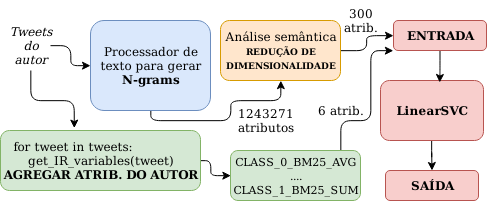
\includegraphics[width=0.75\textwidth]{img/2-daneshvar18-arquitetura-com-ri.png}
    \end{center}
    \vspace{-0.5cm}
    \legend{\ABNTEXfontereduzida \textbf{Fonte:} O autor.}
    \label{fig:2-daneshvar18-arquitetura-com-ri}
\end{figure}

				% Por fim, os 6 atributos de RI agregados por autor foram embutidos ao final da representação dos documentos, resultando em documentos representados por 1243277 dimensões, e posteriormente também foi configurado outro experimento para embutir os atributos de RI somente após a redução de dimensionalidade, resultando em documentos represetados por 306 atributos.
				Por fim, os 6 atributos de RI agregados por autor foram embutidos ao final da representação dos documentos após a redução de dimensionalidade, resultando em documentos represetados por 306 atributos.


		\subsection{Resumo das soluções} \label{sec:ResumoDasSoluções}
			Na Tabela \ref{tab:resumo-soluções} a seguir estão as principais características das soluções selecionadas.

			\begin{table}[!thb]
	%\huge
    \centering
    \caption{Resumo dos detalhes das soluções selecionadas.}
    \begin{adjustbox}{max width={\textwidth},keepaspectratio}%
    \begin{tabular}{|l|c|c|c|c|c|}
        % \toprule
        \hline
        \textbf{Solução}
        & \textbf{Pré-processamento} & \textbf{Núm. atrib.} & \textbf{Redução dim.} 
        & \textbf{Núm. atrib. após}  & \textbf{Classificador}
        \\ \hline
        1\underscore{}bertha        
        & ELMo          & 200 x 1024        & Não
        & 200 x 1024    & CNN (5 cam. esc.) 
        \\ \hline
        4\underscore{}tom
        & GloVe         & 300               & Não
        & 300           & SVC                
        \\ \hline
        2\underscore{}daneshvar18
        & N-gram palavras+caracteres & 1243271           & Sim
        & 300           & LinearSVC          
        \\ 
        \hline
        % \bottomrule
    \end{tabular}
    \end{adjustbox}
    \legend{\ABNTEXfontereduzida \textbf{Fonte:} O autor.}
    \label{tab:resumo-soluções} 
    % \legend{\textbf{Fonte:} O autor.}
\end{table}


	\section{Desempenho das ferramentas de armazenamento e indexação} \label{sec:DesempenhoFerramentas}
		Para cálculo das medidas TIME\_INDEX e TIME\_QUERY, conforme sugeridas no Capítulo \ref{ch:MateriaisMétodos}, foi empregada a linguagem de programação Python, utilizada para implementada uma classe chamada \textit{IndexToolManager} que abstrai a indexação e o cálculo das variáveis de RI com as ferramentas. 

		Essa classe foi central para todo o estudo, a utilização dela concentrou as funções para acesso e manipulação, quando disponíveis, aos dados das ferramentas de armazenamento e indexação, centralização das diferentes bibliotecas do Python já disponíveis para interagir com o ArangoDB e com o Elasticsearch, python-arango e elasticsearch-py respectivamente. 
		Trechos da implementação da classe \textit{IndexToolManager} estão no Apêndice \ref{apên:implementação-indextoolmanager}.
		% Adicionar funcṍes importantes e citar código aqui?
		\subsection{Tempo de indexação}
			Para cálculo da medida TIME\_INDEX foi criado um script Python nomeado \texttt{time\_index.py}, o qual utilizou da classe \textit{IndexToolManager} em duas funções feitas para executar a indexação dos bancos de dados, DB\_AUTHORPROF e DB\_HYPERPARTISAN, nas 3 ferramentas, ArangoDB, Elasticsearch e Zettair.
			A função principal do script \texttt{time\_index.py} possui nome \textit{measure\_TIME\_INDEX}, e um trecho do código que implementa essa função pode ser visto a seguir no Código \ref{cmd:function-measure-time-index}.

			\sourcecodenolinenos{Função \textit{measure\_TIME\_INDEX} do script \texttt{time\_index.py}.}{function-measure-time-index}{python}{function-measure-TIME-INDEX.py}
			% \sourcecodeinline{python}{codes/function-measure-TIME-INDEX.py}

			Essa função é responsável por efetuar uma chamada à função \textit{index} com os parâmetros de tipo de indexação, corpus a ser indexado, e qual a ferramenta utilizada nessa indexação, além de uma identificação do experimento.
			A função \textit{index}, que pode ser vista no Apêndice \ref{apên:função-index}, faz os devidos tratamentos para chamar os métodos da classe \textit{IndexToolManager} responsáveis por fazer a indexação dos documentos do corpus especificado utilizando a ferramenta especificada, isso enquanto mensura o tempo que cada indexação levou e registra todas as operações num arquivo de texto.

			% Colocar o código fonte da função index aqui?
			
			Como as ferramentas ArangoDB e Elasticsearch se assemelham bastante a sistemas gerenciadores de bancos de dados completos, preparados, inclusive, para distribuição geográfica dos dados, há de ser citada essa grande diferença deles para o Zettair, este último que é somente um sistema para indexação em lotes e consulta local dos dados, não permitindo, por exemplo, adição de novos documentos em um índice. 
			A ação de inserção unitária é um procedimento comum em SGBDs. 			

			A operação de indexação foi executada de dois modos, em lote e unitária, sendo que o Zettair só permite a inserção em lote. 
			Na Figura \ref{fig:time-index-bulk} pode ser visto o tempo mensurado, em milissegundos gastos por documento, para inserção em lote dos documentos dos corpus em cada ferramenta.

			\begin{figure}[h]
    \centering
    \caption{Medidas de desempenho TIME\_INDEX mensuradas para as ferramentas de armazenamento e indexação, com inserções feitas em lote.}
    \begin{center}
        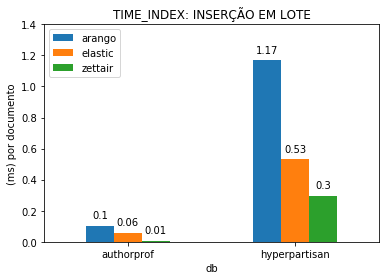
\includegraphics[width=0.75\textwidth]{img/time-index-bulk.png}
    \end{center}
    \vspace{-0.5cm}
    \legend{\ABNTEXfontereduzida \textbf{Fonte:} O autor.}
    \label{fig:time-index-bulk}
\end{figure}

			O Zettair é a ferramenta mais rápida para completar a indexação de ambos os corpus selecionados, levando somente 2,29 segundos para indexar os 300 mil documentos do corpus DB\_AUTHORPROF, menos de 0,01 milissegundos por documento.
			Dentre os SGBDs avaliados, o Elasticsearch supera o ArangoDB para inserções em lote, gastando 17,61 segundos para indexar os 300 mil \textit{tweets}, cerca de 0,06 milissegundos por documento.
			Nota-se ainda que a indexação do corpus DB\_HYPERPARTISAN é mais lenta quando se considera o tempo por documento inserido, porque, apesar do corpus DB\_AUTHORPROF ter um número bem maior de documentos, 300 mil em comparação com 645, cada artigo do DB\_HYPERPARTISAN é bem mais extenso que qualquer dos \textit{tweets} do DB\_AUTHORPROF.
			A mesma relação de velocidade entre as ferramentas observada para as inserções feitas com os documentos do DB\_AUTHORPROF se mantem para as inserções feitas com os documentos do DB\_HYPERPARTISAN, o Zettair é o mais rápido, e, dentre os SGBDs, o Elasticsearch é mais rápido que o ArangoDB.
			
			Para operação de inserção unitária, avaliada somente com o ArangoDB e Elasticsearch, foi levado em conta o tempo total para indexação de todos os documentos de cada corpus, inseridos em sequência, e posteriormente esses valores mensurados foram divididos pelo número de documentos.
			Na Figura \ref{fig:time-index-individual} estão dispostos os tempos totais para indexação de todos os documentos dos corpus com ambas as ferramentas. 

			\begin{figure}[h]
    \centering
    \caption{Medidas de desempenho TIME\_INDEX mensuradas para as ferramentas de armazenamento e indexação, com inserções unitárias.}
    \begin{center}
        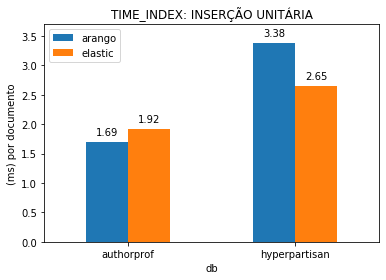
\includegraphics[width=0.75\textwidth]{img/time-index-individual.png}
    \end{center}
    \vspace{-0.5cm}
    \legend{\ABNTEXfontereduzida \textbf{Fonte:} O autor.}
    \label{fig:time-index-individual}
\end{figure}

			O ArangoDB teve um melhor desempenho para as inserções dos documentos do DB\_AUTHORPROF, com 1,69 milissegundos por documento, em contraste aos 1,92 milissegundos por documento do Elasticsearch.
			Porém, o Elasticsearch foi mais rápido para inserção dos documentos do DB\_HYPERPARTISAN, com 2,65 milissegundos por documento contra 3,38 milissegundos por documento do ArangoDB.		

			Percebe-se então que o ArangoDB se saiu um pouco melhor que o Elasticsearch na inserção de grande quantidade de documentos pequenos em sequência, evidenciado pelos tempos de inserção unitária da Figura \ref{fig:time-index-individual}.
			E pode-se supor que isto é derivado de alguma sobrecarga na operação de inserção unitária do Elasticsearch, ou talvez no custo de recálculo do índice que varia com o tamanho dos documentos inseridos, porém com um custo inicial maior, já que para inserção unitária dos documentos do DB\_HYPERPARTISAN, que são artigos extensos, o Elasticsearch teve melhor desempenho.
				
			No geral, o desempenho da indexação por inserção unitária fica abaixo da por inserção em lotes, como era esperado.

		\subsection{Tempo de consulta}
			Para medir o TIME\_QUERY utilizando cada ferramenta durante a execução das soluções foi necessário adaptar os códigos das soluções para fazer o registro do tempo que cada consulta, e posterior geração dos atributos de RI, levou.

			A fim de facilitar a geração dos atributos, foram implementados métodos na classe \textit{IndexToolManager} para que: dado um texto, seja cálculo direto das variáveis de RI já com as ferramentas específicas, como por exemplo o método \textit{arango\_get\_IR\_variables}.
			A utilização desses métodos pode ser visto no trecho disposto a seguir do script Python \texttt{feat\_GloVe.ipynb} da solução 4\_tom adaptada.

			% \sourcecodenolinenos{Trecho da adaptação feita ao script \texttt{feat\_GloVe.ipynb} da solução 4\_tom.}{time-query-calculation-4-tom}{python}{time-query-calculation-4-tom.py}
			\begin{listing}[H]
				\refstepcounter{sourcecode}
				\captionof{listing}{Trecho da adaptação feita ao script \texttt{feat\_GloVe.ipynb} da solução 4\_tom.\label{cmd:time-query-calculation-4-tom}}
			\end{listing}
			\vspace{-1.0cm}
			\inputminted[bgcolor=bg, 
			tabsize=4, baselinestretch=1, breaklines]{python}{codes/time-query-calculation-4-tom.py}
			\vspace{-1.0cm}
			\Ididthis

			Neste trecho, Código \ref{cmd:time-query-calculation-4-tom}, \textit{toolTest} é uma instância da classe \textit{IndexToolManager} com \textit{top-$k$} igual a 100. 
			Esta classe que é responsável pelo cálculo das variáveis de RI, e o tempo de consulta leva em conta esse cálculo, como fica exposto pela posição das variáveis \textit{initial} e \textit{final}.

			O mesmo tipo de adaptação feito para a solução 4\_tom foi feito para as demais, e as medidas coletadas estão dispostas na Figura \ref{fig:time-query}.

			\begin{figure}[h]
    \centering
    \caption{Medidas de desempenho TIME\_QUERY mensuradas para consulta e criação dos 6 atributos de RI sugeridos, utilizando as ferramentas de armazenamento e indexação.}
    \vspace{-0.5cm}
    \begin{center}
        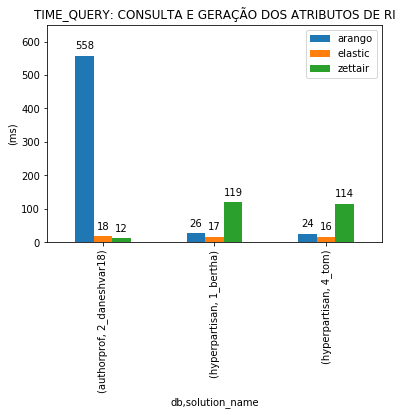
\includegraphics[scale=0.75]{img/time-query.png}
    \end{center}
    \vspace{-0.5cm}
    \legend{\ABNTEXfontereduzida \textbf{Fonte:} O autor.}
    \label{fig:time-query}
\end{figure}

			% Zettair, colocar detalhe dos modos de operação para consulta, iterativa e consulta única

			Ao ver os resultados percebe-se uma discrepância entre os resultados do Zettair nos dois corpus, levando somente 12 milissegundos para o cálculo dos atributos de RI no corpus  corpus DB\_AUTHORPROF e mais de 110 milissegundos para as soluções do corpus DB\_HYPERPARTISAN.
			Isso acontece pois o Zettair possui dois modos de operação para consultas, o 
			\begin{enumerate*}[label=(\alph*)]
				\item modo iterativo e o 
				\item modo de consulta única
			\end{enumerate*}.
			Em ambos os modos o Zettair efetua uma etapa de inicialização, copiando o índice gerado para a memória, e para efetuar consultas em série o modo iterativo é o ideal, no entanto ele possui uma limitação não documentada de cerca de 2048 caracteres nas consultas, como no corpus DB\_AUTHORPROF todos os documentos são pequenos, portanto menores que esse limite, as consultas para gerar os atributos de RI com o Zettair puderam ser executadas no modo iterativo.
			No entanto, para o corpus DB\_HYPERPARTISAN isso não foi possível pois diversos  documentos ultrapassam essa limitação de 2048 caracteres, portanto, para este corpus, as consultas realizadas com o Zettair utilizaram o modo de consulta única.

			A outra surpresa foi o ArangoDB, que levou 558 milissegundos para efetuar cada consulta no corpus DB\_AUTHORPROF, o que indica que seu algoritmo para cálculo do BM25 tem um custo de desempenho proporcional ao número de documentos indexados no banco de dados, pois o corpus DB\_AUTHORPROF possui 300 mil documentos indexados, e o DB\_HYPERPARTISAN somente 430.
			Enquanto isso, o Elasticsearch teve desempenho similar para cálculo dos atributos de RI nos dois corpus, chegando no máximo a 18 milissegundos por consulta no corpus DB\_AUTHORPROF.

			O Zettair é a ferramenta mais rápida para a consulta e geração dos atributos de RI no corpus DB\_AUTHORPROF, porém o Elasticsearch é a melhor ferramenta, em quesito geral de tempo de consulta, devido à limitação do tamanho de documento do modo iterativo do Zettair.

	\section{Desempenho dos classificadores com atributos de RI} \label{sec:DesempenhoClassificadores}
		O desempenho dos classificadores foi mensurado conforme as medidas CLF\_ACC e CLF\_F1 estabelecidas na Subseção \ref{subsec:Desempenho-de-classificador} do Capítulo \ref{ch:MateriaisMétodos}, esses valores foram coletados reproduzindo as soluções originais e então reproduzindo as soluções com as adaptações para incluir os atributos de RI gerados por cada uma das ferramentas.

		A seguir são apresentados as medidas coletadas para as soluções dos corpus.

		\subsection{DB\_HYPERPARTISAN}
			Antes da adaptação das soluções selecionadas foi necessário reproduzi-las, no entanto, como o conjunto de validação da competição de 628 não foi disponibilizado ao público e foi necessário fazer o \textit{holdout} no conjunto de treinamento, não é possível comparar diretamente os resultados finais divulgados na página da competição com os obtidos.
			Pois, para submissão dos classificadores finais para a da competição, ambas as soluções 1\_bertha e 4\_tom treinaram seus classificadores com os 645 artigos e os resultados de acurácia e $F_1$-score disponíveis no ranking da competição foram calculados para as predições feitas nos 628 exemplos do conjunto de validação.
			Além disso, outro problema é que o script Python da solução 1\_bertha disponibilizado online não possuia números aleatórios fixos, o que torna praticamente impossível reproduzir a mesma solução que foi submetida pela equipe para a competição.

			Encontram-se na Tabela \ref{tab:reprodução-db-hyperpartisan} as medidas divulgadas na página da competição \textit{SemEval 2019} \cite{PAN_HNDLEADERBOARD_2019} e as reproduções feitas com treinamento em 430 artigos e validação nos 215 restantes.

			\begin{table}[!thb]
	%\huge
    \centering
    \caption{Comparação das medidas das soluções do corpus DB\underscore{}HYPERPARTISAN divulgadas pelas competição e das reproduções.}
    \begin{adjustbox}{max width={\textwidth},keepaspectratio}%
    \begin{tabular}{|l|c|c|c|c|c|}
        % \toprule
        \hline
        \multirow{2}{*}{\textbf{Solução}}
        & \multicolumn{2}{|c|}{\textbf{Acurácia}}
        & \multicolumn{2}{|c|}{\textbf{$F_1$-score}}
        \\ \cline{2-5}    
        & Competição    & Reprodução
        & Competição    & Reprodução 
        \\ \hline
        1\underscore{}bertha        
        & 0,822         & 0,814
        & 0,809         & 0,762
        \\ \hline
        4\underscore{}tom
        & 0,806         & 0,809
        & 0,790         & 0,707              
        \\ 
        \hline
        % \bottomrule
    \end{tabular}
    \end{adjustbox}
    \legend{\ABNTEXfontereduzida \textbf{Fonte:} O autor.}
    \label{tab:reprodução-db-hyperpartisan} 
    % \legend{\textbf{Fonte:} O autor.}
\end{table}


			Após essa validação que não há nada de muito errado com as soluções reproduzidas em comparação com os resultados divulgados pela competição, pois os resultados reproduzidos ficam dentro do esperado para um conjunto de treinamento reduzido, as soluções foram adaptadas para incluir os atributos de RI conforme o descrito nas seções anteriores.
			Na Figura \ref{fig:clf-acc-bars-hyperpartisan} estão dispostas as medidas CLF\_ACC para ambas as soluções.
			
			\begin{figure}[h]
    \centering
    \caption{Desempenho CLF\_ACC das soluções do corpus DB\_HYPERPARTISAN.}
    \vspace{-0.5cm}
    \begin{center}
        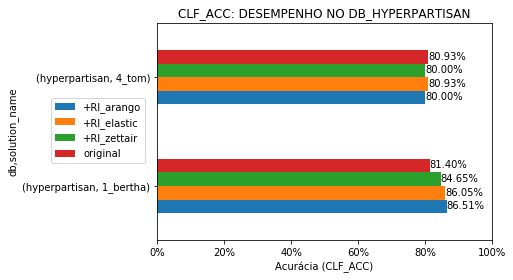
\includegraphics[scale=0.75]{img/clf-acc-bars-hyperpartisan.png}
    \end{center}
    \vspace{-0.5cm}
    \legend{\ABNTEXfontereduzida \textbf{Fonte:} O autor.}
    \label{fig:clf-acc-bars-hyperpartisan}
\end{figure}

			E na Figura \ref{fig:clf-f1-bars-hyperpartisan} estão dispostas as medidas CLF\_F1.
			
			\begin{figure}[h]
    \centering
    \caption{Desempenho CLF\_F1 das soluções do corpus DB\_HYPERPARTISAN.}
    \vspace{-0.5cm}
    \begin{center}
        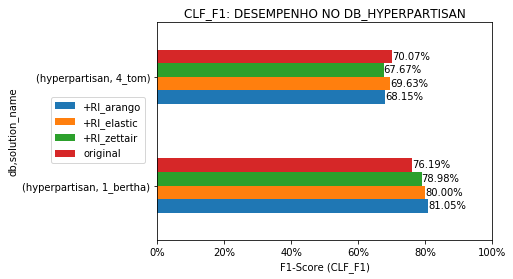
\includegraphics[scale=0.75]{img/clf-f1-bars-hyperpartisan.png}
    \end{center}
    \vspace{-0.5cm}
    \legend{\ABNTEXfontereduzida \textbf{Fonte:} O autor.}
    \label{fig:clf-f1-bars-hyperpartisan}
\end{figure}

			A adição dos atributos de RI proporciona ganho de acurácia e também de $F_1$-Score para a solução 1\_bertha, alcançando valores maiores até mesmo que os finais da competição com acurácia de $0,8651$ ($86,51\%$) e $F_1$-Score de $0,8105$ ($81,05\%$) quando adicionados os atributos de RI gerados pelo ArangoDB.
			Já para a solução 4\_tom inicialmente a adição dos atributos de RI não proporciona nenhum ganho de acurácia ou $F_1$-Score, pelo contrário, com todas as ferramentas o $F_1$-Score foi menor ao adicionar os atributos de RI, e somente com os atributos de RI do Elasticsearch que a acurácia se manteve a mesma, com o ArangoDB e com o Zettair houve também diminuição da acurácia do classificador da solução 4\_tom.

			Deve ser observado um detalhe importante da solução 4\_tom, que é o classificador utilizado e o modo escolhido para definição dos parâmetros desse classificador pela equipe, que no caso foi o classificador SVC e na elaboração de sua solução a equipe avaliou diferentes valores do parâmetro C do classificador e escolheu o valor de C com melhor resultado nesse teste, que foi $C = 0,9$.
			Como o conjunto de treinamento para submissão da equipe consistiu de todos os 645 artigos, e na reprodução feita para este estudo isso não pode ser feito devido à necessidade de um conjunto isolado de validação, foi feita a suposição que o melhor valor de C para a reprodução da solução seria diferente, pois o conjunto de treinamento da reprodução possui somente 430 artigos.
			
			Nas Figuras \ref{fig:clf-acc-4-tom} e \ref{fig:clf-f1-4-tom} estão plotadas as medidas CLF\_ACC e CLF\_F1 obtidas com a reprodução da solução 4\_tom com valores de C na faixa de 0,00001 a 10,0.
			
			\begin{figure}[h]
    \centering
    \caption{Desempenho CLF\_ACC da solução 4\_tom para diferentes valores de refinamento da função custo, parâmetro C do classificador SVC.}
    \vspace{-0.5cm}
    \begin{center}
        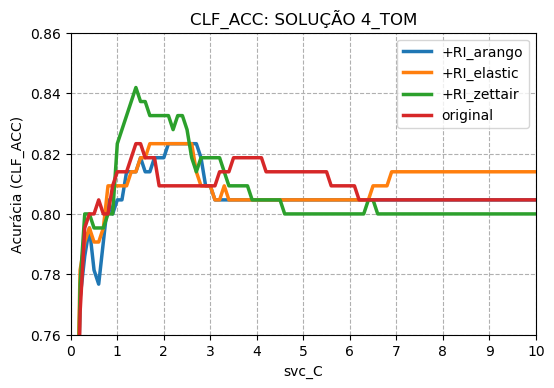
\includegraphics[scale=0.75]{img/clf-acc-4-tom.png}
    \end{center}
    \vspace{-0.5cm}
    \legend{\ABNTEXfontereduzida \textbf{Fonte:} O autor.}
    \label{fig:clf-acc-4-tom}
\end{figure}

			\begin{figure}[h]
    \centering
    \caption{Desempenho CLF\_F1 da solução 4\_tom para diferentes valores de refinamento da função custo, parâmetro C do classificador SVC.}
    \vspace{-0.5cm}
    \begin{center}
        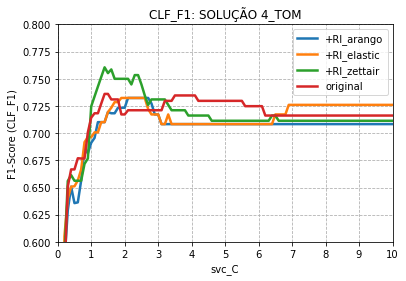
\includegraphics[scale=0.75]{img/clf-f1-4-tom.png}
    \end{center}
    \vspace{-0.5cm}
    \legend{\ABNTEXfontereduzida \textbf{Fonte:} O autor.}
    \label{fig:clf-f1-4-tom}
\end{figure}
			
			Uma rápida análise dos gráficos permite perceber que os melhores valores do parâmetro C agora se encontram na faixa de 1,0 a 3,0 para as reproduções, tanto em termos de CLF\_ACC quanto de CLF\_F1.
			O valor de $C = 0,9$ de fato não está entre os melhores possíveis para o classificador.
			
			Nota-se que, mesmo com a adição dos atributos de RI, utilizando tanto o ArangoDB quanto o Elasticsearch, o classificador em nenhum momento consegue superar o melhor valor de C do classificador original, porém, com adição dos atributos de RI gerados pelo Zettair, ele atinge os valores de $\text{CLF\_ACC} = 0,8419$ e $\text{CLF\_F1} = 0,7606$ quando $C = 1,4$.
			Os valores máximos atingidos com os respectivos valores de C estão dispostos na Tabela \ref{tab:reprodução-4-tom-c}.

			\begin{table}[!thb]
	%\huge
    \centering
    \caption{Melhores valores de CLF\underscore{}ACC e CLF\underscore{}F1 do classificador SVC da solução 4\underscore{}tom após reproduzida com diferentes valores de C.}
    \begin{adjustbox}{max width={\textwidth},keepaspectratio}%
    \begin{tabular}{|l|c|c|c|}
        % \toprule
        \hline
        \textbf{Solução}
        & \textbf{C}
        & \textbf{Acurácia}
        & \textbf{$F_1$-score}
        \\ \hline
        original        
        & 1,4   & 0,8233   & 0,7361 
        \\ \hline
        +RI\underscore{}arango
        & 2,1   & 0,8233    & 0,7324          
        \\ \hline
        +RI\underscore{}elastic
        & 1,9   & 0,8233    & 0,7324        
        \\ \hline
        +RI\underscore{}zettair
        & 1,4   & \textbf{0,8419}    & \textbf{0,7606}          
        \\ 
        \hline
        % \bottomrule
    \end{tabular}
    \end{adjustbox}
    \legend{\ABNTEXfontereduzida \textbf{Fonte:} O autor.}
    \label{tab:reprodução-4-tom-c} 
    % \legend{\textbf{Fonte:} O autor.}
\end{table}


			Observa-se então que a adição dos atributos de RI, utilizando o Zettair para gerá-los, oferece um ganho de desempenho para o classificador SVC da solução 4\_tom quando efetuada a otimização de hiperparâmetros.
			Porém, ainda assim o classificador SVC não consegue superar os resultados obtidos com o classificar CNN da solução 1\_bertha ao adicionar os parâmetros de RI com quaisquer das ferramentas.
			O que pode parecer um tanto estranho, já que na solução 4\_tom somente o Zettair produziu ganho de desempenho do classificador.
			Talvez isso esteja relacionado ao modo de classificação final utilizado pela solução 1\_bertha, no qual é feito o \textit{ensemble} (junção) dos três melhores modelos de qualquer época durante o treinamento da CNN, é possível que os atributos de RI não sejam os responsáveis pelo ganho de desempenho observado na solução 1\_bertha, mas somente a iteração diferente, devido a alteração no conjunto de atributos feita por cada ferramenta, tenha gerado modelos que tenham melhor desempenho no \textit{ensemble}.
			% Nota de rodapé sobre ensemble?
			Pois, mesmo com a fixação da semente do gerador de número aleatório, como os valores dos atributos de RI são alterados (já que cada ferramenta sua própria implementação do BM25 com pequenas diferenças entre si), os modelos gerados pela reprodução com adição dos atributos de RI gerados pelo Zettair é diferente dos gerados pelo Elasticsearch, que também é diferente dos gerados pelo ArangoDB, e todos estes também são diferentes dos modelos gerados sem adição dos atributos de RI.


		\subsection{DB\_AUTHORPROF}
			A solução 2\_daneshvar18 foi reproduzida sem nenhuma adaptação para comparação com os valores que se encontram na página da competição.
			Na Tabela \ref{tab:reprodução-db-authorprof} está a medida de acurácia divulgada na página da competição \cite{PAN_APCLEF_2018} junto com as medidas da reprodução feitas do mesmo modo que a submissão original, treinamento com os tweets de 3000 autores de língua inglesa e validação com os tweets de 1900 autores de língua inglesa.
			% e a medida $F_1$-score apresentada na descrição da solução pela equipe
			% PAN_APCLEF_2018.

			\begin{table}[!thb]
	%\huge
    \centering
    \caption{Comparação das medidas da solução 2\underscore{}daneshvar18 do corpus DB\underscore{}AUTHORPROF divulgadas pela competição e da reprodução da solução.}
    \begin{adjustbox}{max width={\textwidth},keepaspectratio}%
    \begin{tabular}{|l|c|c|c|c|c|}
        % \toprule
        \hline
        \multirow{2}{*}{\textbf{Solução}}
        & \multicolumn{2}{|c|}{\textbf{Acurácia}}
        & \multicolumn{2}{|c|}{\textbf{$F_1$-score}}
        \\ \cline{2-5}    
        & Competição    & Reprodução
        & Competição    & Reprodução 
        \\ \hline
        2\underscore{}daneshvar18        
        & 0,8221        & 0,822105	
        & --            & 0,820785
        \\ 
        \hline
        % \bottomrule
    \end{tabular}
    \end{adjustbox}
    \legend{\ABNTEXfontereduzida \textbf{Fonte:} O autor.}
    \label{tab:reprodução-db-authorprof} 
    % \legend{\textbf{Fonte:} O autor.}
\end{table}


			Ao truncar o resultado de acurácia da solução reproduzida em 4 dígitos, confirmamos que o mesmo valor divulgado na página da competição é o obtido ao reproduzir a solução.
			Tanto a página da competição quanto o artigo de descrição da solução \cite{daneshvar:2018} só mencionam a acurácia da solução, portanto não há como comparar o $F_1$-score obtido ao reproduzir a solução.

			Depois da validação inicial da solução 2\_daneshvar por meio da reprodução dos resultados da competição, ela foi adaptada para incluir os atributos de RI junto aos atributos de entrada do classificador antes da redução de dimensionalidade.
			As medições de CLF\_ACC e CLF\_F1 obtidas ao reproduzir a solução incluindo os atributos com as diferentes ferramentas estão dispostas nas Figura \ref{fig:clf-bars-authorprof}.
			%  e \ref{fig:clf-f1-bars-authorprof}.

			\begin{figure}[ht]
    \centering
    \caption{Desempenho CLF\underscore{}F1 e CLF\underscore{}ACC da solução reproduzida para o corpus DB\underscore{}AUTHORPROF.}
    \vspace{-0.5cm}
    \begin{center}
        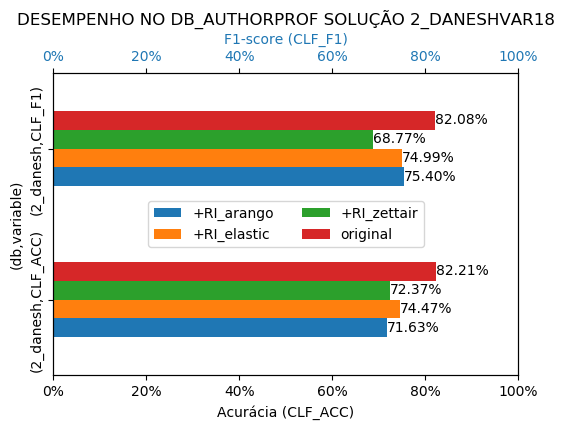
\includegraphics[scale=0.75]{img/clf-bars-authorprof.png}
    \end{center}
    \vspace{-0.5cm}
    \legend{\ABNTEXfontereduzida \textbf{Fonte:} O autor.}
    \label{fig:clf-bars-authorprof}
\end{figure}

			% \begin{figure}[ht]
    \centering
    \caption{Desempenho CLF\underscore{}ACC da solução reproduzida para o corpus DB\underscore{}AUTHORPROF.}
    \vspace{-0.5cm}
    \begin{center}
        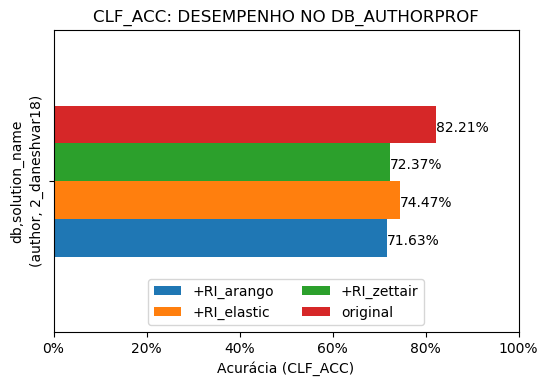
\includegraphics[scale=0.75]{img/clf-acc-bars-authorprof.png}
    \end{center}
    \vspace{-0.5cm}
    \legend{\ABNTEXfontereduzida \textbf{Fonte:} O autor.}
    \label{fig:clf-acc-bars-authorprof}
\end{figure}


			% \begin{figure}[h]
    \centering
    \caption{Desempenho CLF\_F1 da solução reproduzida para o corpus DB\_AUTHORPROF.}
    \vspace{-0.5cm}
    \begin{center}
        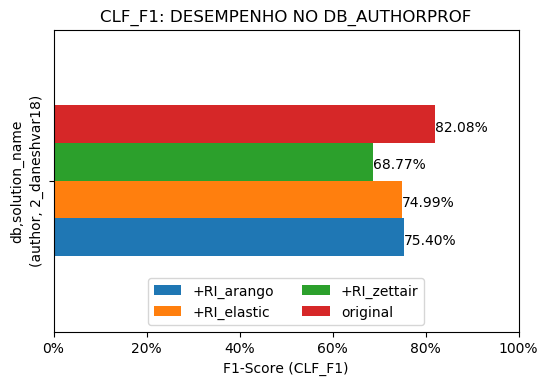
\includegraphics[scale=0.75]{img/clf-f1-bars-authorprof.png}
    \end{center}
    \vspace{-0.5cm}
    \legend{\ABNTEXfontereduzida \textbf{Fonte:} O autor.}
    \label{fig:clf-f1-bars-authorprof}
\end{figure}

			Como pode ser observado nos gráficos, os atributos de RI na verdade provocaram uma perda considerável de desempenho do classificador da solução 2\_daneshvar18, ambas as medidas CLF\_ACC e CLF\_F1 foram menores com a adição dos atributos de RI com quaisquer das ferramentas utilizadas.
			O classificador da solução se trata de um classificador do tipo de Máquinas de Vetor de Suporte, o LinearSVC, e assim como foi feito com a solução 4\_tom anteriormente, pode-se supor que o parâmetro C do classificador, escolhido como o padrão $C = 1,0$ pela equipe da solução 2\_daneshvar18, não se trata do melhor valor possível para os modelos de classificação gerados ao adicionar os atributos de RI.
			Então, trabalhando com essa hipótese, a solução foi reproduzida alterando o valor de C do LinearSVC na faixa de valores de $0,00001$ a $10,0$.
			As medidas coletadas estão plotadas nas Figuras \ref{fig:clf-acc-2-daneshvar18} e \ref{fig:clf-f1-2-daneshvar18}.


			\begin{figure}[ht]
    \centering
    \caption{Desempenho CLF\underscore{}ACC da solução 2\underscore{}daneshvar18 para diferentes valores de refinamento da função custo, parâmetro C do classificador LinearSVC.}
    \vspace{-0.5cm}
    \begin{center}
        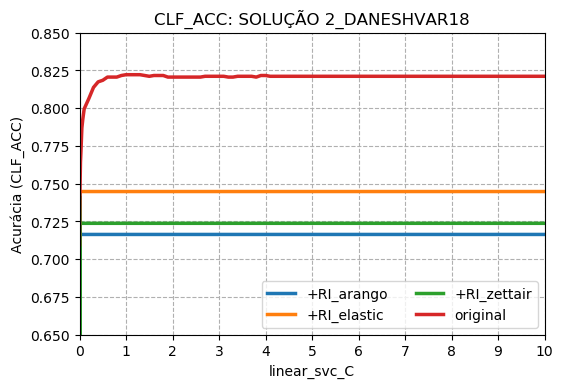
\includegraphics[scale=0.75]{img/clf-acc-2-daneshvar18.png}
    \end{center}
    \vspace{-0.5cm}
    \legend{\ABNTEXfontereduzida \textbf{Fonte:} O autor.}
    \label{fig:clf-acc-2-daneshvar18}
\end{figure}

			\begin{figure}[ht]
    \centering
    \caption{Desempenho CLF\underscore{}F1 da solução 2\underscore{}daneshvar18 para diferentes valores de refinamento da função custo, parâmetro C do classificador LinearSVC.}
    \vspace{-0.5cm}
    \begin{center}
        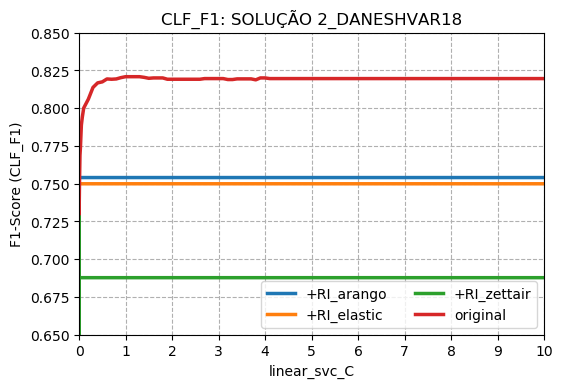
\includegraphics[scale=0.75]{img/clf-f1-2-daneshvar18.png}
    \end{center}
    \vspace{-0.5cm}
    \legend{\ABNTEXfontereduzida \textbf{Fonte:} O autor.}
    \label{fig:clf-f1-2-daneshvar18}
\end{figure}

			Os gráficos de desempenho com diferentes valores de C comprovam que os atributos de RI pioraram os modelos gerados pelo classificador LinearSVC da solução 2\_daneshvar18.
			Pode-se dizer que a introdução dos atributos de RI se trata de uma introdução de ruído que atrapalha o classificador e o impede alcançar os níveis de desempenho atingidos utilizando somente os atributos originais.

			Por que isso ocorreu?
			Ao analisar os atributos originais após a redução de dimensionalidade foi constatado que os valores máximos e mínimos de cada uma das colunas dos 300 atributos estavam na faixa de $-1,0$ a $1,0$ enquanto que os 6 atributos de RI gerados pelas ferramentas estavam na faixa de $8,0$ até a casa dos milhares.
			Os classificadores do tipo SVM atribuem maior importância a atributos com maiores magnitudes conforme o núcleo selecionado \cite{Kumar2014}, e isso estava acontecendo com o núcleo padrão do classificador LinearSVC do sklearn.

			Para tentar resolver o problema foi utilizado o escalonador MinMaxScaler nos 6 atributos de RI para dimensioná-los para a faixa de $-1,0$ a $1,0$. 
			Os medidas coletadas podem ser observadas nas Figuras \ref{fig:clf-acc-2-daneshvar18-ir-scaled} e \ref{fig:clf-f1-2-daneshvar18-ir-scaled}. 

			\begin{figure}[h]
    \centering
    \caption{Desempenho CLF\_ACC da solução 2\_daneshvar18 para diferentes valores de refinamento da função custo, parâmetro C do classificador LinearSVC com atributos de RI escalonados pelo MinMaxScaler.}
    \vspace{-0.5cm}
    \begin{center}
        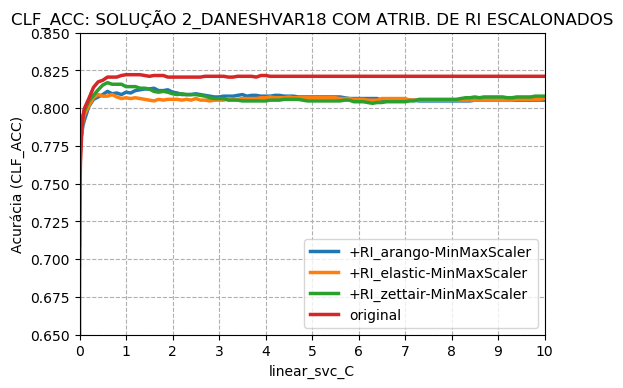
\includegraphics[scale=0.75]{img/clf-acc-2-daneshvar18-ir-scaled.png}
    \end{center}
    \vspace{-0.5cm}
    \legend{\ABNTEXfontereduzida \textbf{Fonte:} O autor.}
    \label{fig:clf-acc-2-daneshvar18-ir-scaled}
\end{figure}

			\begin{figure}[h]
    \centering
    \caption{Desempenho CLF\_F1 da solução 2\_daneshvar18 para diferentes valores de refinamento da função custo, parâmetro C do classificador LinearSVC com atributos de RI escalonados pelo MinMaxScaler.}
    \vspace{-0.5cm}
    \begin{center}
        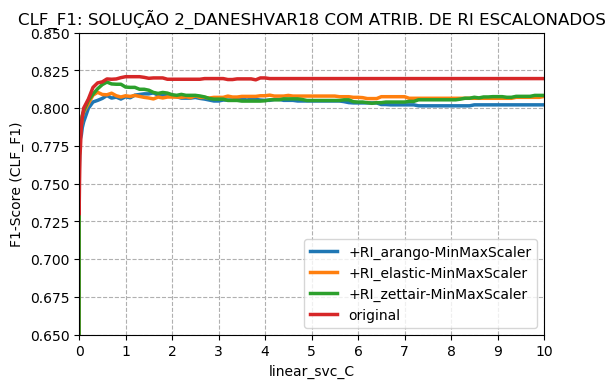
\includegraphics[scale=0.75]{img/clf-f1-2-daneshvar18-ir-scaled.png}
    \end{center}
    \vspace{-0.5cm}
    \legend{\ABNTEXfontereduzida \textbf{Fonte:} O autor.}
    \label{fig:clf-f1-2-daneshvar18-ir-scaled}
\end{figure}

			Apesar do desempenho do classificador da solução 2\_daneshvar18 ter sido maior com os atributos de RI escalonados, como mostra o gráfico da Figura \ref{fig:clf-acc-2-daneshvar18-ir-scaled} em comparação com o da Figura \ref{fig:clf-acc-2-daneshvar18}, ainda assim o desempenho continuou abaixo da reprodução da solução original.
			Na Tabela \ref{tab:reprodução-2-daneshvar18-c} podem ser vistos os valores máximos atingidos com os respectivos valores de C.

			\begin{table}[!thb]
	%\huge
    \centering
    \caption{Melhores valores de CLF\_ACC e CLF\_F1 do classificador LinearSVC da solução 2\_daneshvar18 após reproduzida com diferentes valores de C, com atributos de RI escalonados pelo MinMaxScaler.}
    \begin{adjustbox}{max width={\textwidth},keepaspectratio}%
    \begin{tabular}{|l|c|c|c|}
        % \toprule
        \hline
        \textbf{Solução}
        & \textbf{C}
        & \textbf{Acurácia}
        & \textbf{$F_1$-Score}
        \\ \hline
        original        
        & 1,0   & \textbf{0,822105}   & \textbf{0,820785}
        \\ \hline
        +RI\_arango
        & 1,6   & 0,813158   & 0,810059          
        \\ \hline
        +RI\_elastic
        & 0,4   & 0,808947    & 0,810444
        \\ \hline
        +RI\_zettair
        & 0,6   & 0,816842	    & 0,817227
        \\ 
        \hline
        % \bottomrule
    \end{tabular}
    \end{adjustbox}
    \legend{\ABNTEXfontereduzida \textbf{Fonte:} O autor.}
    \label{tab:reprodução-2-daneshvar18-c} 
    % \legend{\textbf{Fonte:} O autor.}
\end{table}


			Pode-se perceber que o melhor desempenho com os atributos de RI é quando gerado pelo Zettair, no entanto ainda assim fica abaixo da solução original.
			Obtendo acurácia de $81,68\%$ contra $82,22\%$ da original, e $F_1$-score de $81,72\%$ contra $82,08\%$ da original.
	% Fluxograma das alterações feitas nos códigos com exemplos de trechos alterados
	% Rosalvo disse que é para colocar no Apêndice

	% ganho de informação das 6 variáveis nas soluções

	% Citar as técnicas só de um, descrições, citar algum livro ou página

	% Criar rede neural para comparar à solução do DB_AUTHORPROF à parte 


		%--------------------------------------------------------------------------------------
% Este arquivo contém a sua conclusão
%--------------------------------------------------------------------------------------
\chapter{Considerações Finais e Trabalhos Futuros} \label{ch:ConsideraçõesFinais}

% recapitular tudo, qual o propósito
% 1 parágrafo
Esse estudo investigativo buscou avaliar o desempenho de atributos oriundos da área de Recuperação de Informação em tarefas de Mineração de Texto, com enfoque em atributos gerados pela função BM25, por meio de uma metodologia própria.
A geração desses atributos foi subsidiada por ferramentas que implementam a função BM25 e o desempenho dos atributos de RI foi avaliado em dois corpus distintos.
O desempenho das ferramentas de armazenamento e indexação também foi avaliado.
% falar o que vi de fato nos resultados
% -- foi visto que para a base X, Y aconteceu provavelmente  devido a Z
 
Os resultados obtidos com a metodologia proposta mostram que o Zettair foi a ferramenta mais rápida na questão de indexação e também para consultas com textos de tamanho limitado.
O Elasticsearch também apresentou bom desempenho, não possuindo limitações de tamanho do texto nas consultas, e foi o melhor dentre os dois SGBDs testados.
Além disso, ele possui muito mais funcionalidades que o Zettair, que por sua vez não é um SGBD.

Ainda na avaliação de desempenho das ferramentas, percebe-se que o ArangoDB obteve um resultado muito aquém dos demais na medida TIME\underscore{}QUERY para o corpus de 300 mil registros, indicando que as consultas utilizando a função BM25 do ArangoDB são lentas para bancos de dados com grande número de documentos.
% reforçar as melhores ferramentas, porque são resultados de desempenho mais claros

Dentre as soluções selecionadas para reprodução, só foi possível comprovar as medidas do ranking final das competições para a solução 2\underscore{}daneshvar18 do corpus DB\underscore{}AUTHORPROF, para as duas soluções do corpus DB\underscore{}HYPERPARTISAN isso não foi possível pois o conjunto de validação final da competição não foi publicado.
Contudo, as soluções do DB\underscore{}HYPERPARTISAN selecionadas mantiveram a relação de posição quando reproduzidas, com a solução 1\underscore{}bertha obtendo melhor acurácia e melhor $F_1$-score do que a solução 4\underscore{}tom.

Na avaliação de desempenho dos classificadores adicionando os atributos de RI, a Rede Neural Convolucional (1\underscore{}bertha) apresentou o maior ganho de desempenho, saltando de uma acurácia de $81,40\%$ para $86,51\%$ e $F_1$-score de $76,19\%$ para $81,05\%$ ao utilizar o ArangoDB para gerar os atributos de RI.
A adição dos atributos de RI gerados por quaisquer ferramentas proporcionou ganho de desempenho à CNN da solução 1\underscore{}bertha para o corpus DB\underscore{}HYPERPARTISAN, porém, não houve qualquer ganho de desempenho ao adicionar os atributos de RI ao classificador SVC da solução 4\underscore{}tom devido à fixação do parâmetro de refinamento da função custo do SVC na solução original.

Uma análise e seleção dos parâmetros do classificador SVC mostrou que adicionar os atributos de RI gerados pelo Zettair produz um ganho de desempenho de acurácia de $82,33\%$ para $84,19\%$ e $F_1$-score de $73,61\%$ para $76,06\%$ quando o melhor valor do parâmetro C é selecionado.
Já a adição dos atributos gerados pelas outras ferramentas não proporcionou ganho.

Quanto ao corpus DB\underscore{}AUTHORPROF, o classificador LinearSVC da solução 2\underscore{}daneshvar18 não obteve nenhum ganho de desempenho ao serem adicionados os atributos de RI, nem mesmo ao ser feita a análise e seleção do parâmetro C do classificador.
Uma investigação posterior revelou que na verdade a magnitude dos atributos de RI era bem maior que a dos atributos originais, prejudicando o classificador LinearSVC.
No entanto, mesmo com o reparo de magnitude por meio do escalonador MinMaxScaler, e nova análise e seleção do parâmetro C do classificador, não foi obtido nenhum ganho de desempenho ao adicionar os atributos de RI à solução 2\underscore{}daneshvar18.

Então, conclui-se que os 6 atributos de RI sugeridos nesse estudo proporcionaram ganho de desempenho somente para classificações do corpus DB\underscore{}HYPERPARTISAN, um corpus pequeno com documentos extensos.
Os atributos de RI funcionaram melhor com o classificador CNN, e para o classificador SVC somente o Zettair proporcionou ganho de desempenho.
No corpus DB\underscore{}AUTHORPROF, um corpus grande com documentos curtos, com o classificador LinearSVC, os atributos de RI causaram perda de desempenho.
Esses resultados divergem da principal conclusão dos estudos de \citeonline{WEREN_MESTRADO_2014}, onde ele afirma que ``os atributos oriundos de recuperação de informação propostos [$\cdots$] produzem as melhores previsões'', já que utilizar somente os atributos originais da solução apresentou melhores resultados do que adicionar os atributos de RI.

Para corroborar o ganho de desempenho, ou não, dos atributos de RI sugeridos, e em quais casos eles valem a pena ser utilizados, são necessários mais testes pois os resultados aqui obtidos não são unânimes.
Esses testes podem ser feitos com outros classificadores nesses mesmos corpus e também em diferentes corpus, corpus grandes com documentos extensos e corpus pequenos com documentos pequenos. 
Podem ser pensados também testes com diferentes valores de top-$k$ e parâmetros $k_1$, $k_3$ e $b$ para cálculo dos atributos de RI.

% limitações do que foi feito

% 
\section{Trabalhos futuros}
    Para trabalhos futuros está planejada uma maior análise exploratória dos parâmetros da solução 2\underscore{}daneshvar18, reproduzindo a solução com maiores variações nos parâmetros do classificador LinearSVC, inclusive com alteração do núcleo do mesmo, para verificar se alguma configuração dele possui desempenho superior constante ao serem adicionados os atributos de RI. 
    Isso não foi feito neste estudo devido à limitação temporal para executar todas as variações necessárias para chegar a mais conclusões, mas alguns resultados já estão guardados.
    % mas algumas das diferentes configurações já foram executadas ou reproduzidas

    Quanto maior o número de soluções reproduzidas para cada corpus melhor, mas trabalhar com um mínimo talvez seja o ideal, então para todas as reproduções futuras é bom tomar como base no mínimo duas soluções, ou classificadores distintos, por corpus, para efetuar as comparações.
    Então, em um trabalho futuro imediato planeja-se reproduzir mais uma das soluções do corpus DB\underscore{}AUTHORPROF disponíveis online.

    Como mencionado antes, trabalhos futuros podem também trabalhar somente analisando diferentes valores que influenciem somente nos atributos de RI gerados, o top-$k$ e os parâmetros $k_1$, $k_3$ e $b$ reproduzindo-os para os mesmos corpus.

    Além disso, uma outra possibilidade de estudo, é o maior isolamento do índice de geração dos atributos de RI do conjunto de treinamento por meio da separação dos corpus em 3 pedaços.
    Nessa separação o primeiro pedaço seria utilizado para para treinamento do classificador, o segundo pedaço seria utilizado como o índice para geração dos atributos derivados da função BM25 para o primeiro pedaço, e o terceiro pedaço ficaria para teste/validação do classificador.

% \lipsum[55]

	\postextual

		\justify
		\bibliography{tex/references}
% 		\begin{anexosenv}
    \chapter{Comandos seriais da estação meteorológica \textit{Vantage Vue™}} \label{anex:anexo1}

    \inputminted[bgcolor=bg, 
    tabsize=4, baselinestretch=1, breaklines]{python}{codes/time-query-calculation-4-tom.py}
    
    \begin{center}
        \scalefont{0.85}
        \begin{longtable}{ll}
        \caption{Comandos seriais suportados pela estação meteorológica \textit{Vantage Vue™}}\\
        \hline
        \multicolumn{1}{c}{\textbf{Instrução}} & \multicolumn{1}{c}{\textbf{Descrição}} \\ \hline
        \endfirsthead

        \multicolumn{2}{c}%
        {{\bfseries \tablename\ \thetable{} -- Continuação da página anterior}} \\

        \hline
        \multicolumn{1}{c}{\textbf{Instrução}} & \multicolumn{1}{c}{\textbf{Descrição}} \\ \hline
        \endhead

        \multicolumn{2}{r}{{Continua na próxima página}} \\
        \endfoot

        \endlastfoot

        \multicolumn{2}{c}{\cellcolor{gray!25}\textbf{Comandos de teste}}                                                   		 \\ \hline
        \textbf{TESTE}                            & Envia a \textit{string} "TEST\textbackslash n" de volta  \\ \hline
        \textbf{WRD}                        & Responde com o tipo de estação meteorológica \\ \hline
        \textbf{RXCHECK}                        & Responde com o diagnóstico do Console \\ \hline
        \textbf{RXTEST}                       & Muda a tela do console de \textit{"Receiving from"} para tela de dados atuais                                                        \\ \hline
        \textbf{VER}                           & Responde com a data do \textit{firmware}                                                             \\ \hline
        \textbf{RECEIVERS}                    & Responde com a lista das estações que o console "enxerga" \\ \hline
        \textbf{NVER}                       & Responde com a versão do \textit{firmware}                                                             \\ \hline
        \multicolumn{2}{c}{\cellcolor{gray!25}\textbf{Comandos de dados atuais}}                                             \\ \hline
        \textbf{LOOP}                     & Responde com a quantidade de pacotes especificada a cada 2s        \\ \hline
        \textbf{LPS}                & Responde a cada 2s com a quantidade de pacotes diferentes especificada          \\ \hline
        \textbf{HILOWS}                & Responde com todo os dados de \textit{high/low}                 \\ \hline
        \textbf{PUTRAIN}                      & Seta a quantidade anual de precipitação \\ \hline
        \textbf{PUTET}                 & Seta a quantidade anual de evapotranspiração        \\ \hline
        \multicolumn{2}{c}{\cellcolor{gray!25}\textbf{Comandos de \textit{download}}}                                     		 \\ \hline
        \textbf{DMP}                 & Faz o \textit{download} de todo o arquivo de memória \\ \hline
        \textbf{DMAFT}                   & Faz o \textit{download} de todo o arquivo de memória após a data especificada \\ \hline
        \multicolumn{2}{c}{\cellcolor{gray!25}\textbf{Comandos da EEPROM}}                                     		 \\ \hline
        \textbf{GETEE}                 & Lê toda a memória EEPROM \\ \hline
        \textbf{EEWR}                   & Escreve um \textit{byte} de dados à partir do endereço especificado                                   \\ \hline
        \textbf{EERD}                   & Lê a quantidade de dados especificada iniciando no endereço especificado                                   \\ \hline
        \textbf{EEBWR}                   & Escreve os dados na EEPROM                                    \\ \hline
        \textbf{EEBRD}                   & Lê os dados da EEPROM \\ \hline
        \multicolumn{2}{c}{\cellcolor{gray!25}\textbf{Comandos de calibração}}                                     		 \\ \hline
        \textbf{CALED}                 & Envia os dados da temperatura e umidade corrente para atribuir à calibração \\ \hline
        \textbf{CALFIX}                   & Atualiza o \textit{display} quando os números de calibração mudam\\ \hline
        \textbf{BAR}                   & Seta os valores da elevação e o \textit{offset} do barômetro quando a localização é alterada                                   \\ \hline
        \textbf{BARDATA}                   & Mostra os valores atuais da calibração do barômetro                                   \\ \hline \\
        \multicolumn{2}{c}{\cellcolor{gray!25}\textbf{Comandos de limpeza}}                                     		 \\ \hline
        \textbf{CLRLOG}                 & Limpa todo o arquivo de dados                                                       \\ \hline
        \textbf{CLRALM}                   & Limpa todos os limiares dos alarmes                                   \\ \hline
        \textbf{CLRCAL}                   & Limpa todos os \textit{offsets} da calibração da temperatura e da umidade \\ \hline
        \textbf{CLRGRA}                   & Limpa o gráfico do console \\ \hline
        \textbf{CLRVAR}                   & Limpa o valor da precipitação ou da evapotranspiração \\ \hline
        \textbf{CLRHIGHS}                   & Limpa todos os valores de pico diários, mensais ou anuais                                   \\ \hline
        \textbf{CLRLOWS}                   & Limpa todos os valores de mínimos diários, mensais ou anuais \\ \hline
        \textbf{CLRBITS}                   & Limpa os \textit{bits} de alarme ativos                                  \\ \hline
        \textbf{CLRDATA}                   & Limpa todos os dados atuais                                   \\ \hline
        \multicolumn{2}{c}{\cellcolor{gray!25}\textbf{Comandos de configuração}}                                     		 \\ \hline
        \textbf{BAUD}                 & Atribui o valor do \textit{baudrate} do console                                                       \\ \hline
        \textbf{SETTIME}                   & Define a data e a hora do console                                   \\ \hline
        \textbf{GAIN}                   & Define o ganho do receptor de rádio                                   \\ \hline
        \textbf{GETTIME}                   & Retorna a hora e a data atual do console                                   \\ \hline
        \textbf{SETPER}                   & Define o intervalo de arquivamento                                   \\ \hline
        \textbf{STOP}                   & Desabilita a criação dos registros                                   \\ \hline
        \textbf{START}                   & Habilita a criação dos arquivos \\ \hline
        \textbf{NEWSETUP}                   & Reinicia o console após alguma configuração nova                                  \\ \hline
        \textbf{LAMPS}                   & Liga ou desliga as lâmpadas do console \\ \hline

        %\label{tab:6}
        \end{longtable}
        % \fonte{\citeonline{VSPDOC} (Traduzido).}
    \end{center}


\end{anexosenv}

		% ----------------------------------------------------------
% Apêndices
% ----------------------------------------------------------
% ---
% Inicia os apêndices
% ---
\begin{apendicesenv}
% Imprime uma página indicando o início dos apêndices
    \partapendices
    
    % ----------------------------------------------------------
    \chapter{Trecho de código: função \textit{index}} \label{apên:função-index}
    % ----------------------------------------------------------
    O código completo da função \textit{index} pode ser encontrado no seguinte arquivo disponível na internet: \hyperlink{https://github.com/ruanmed/tcc-ii-ir-features-text-mining/blob/master/tool-testing/time-index.py}{https://github.com/ruanmed/tcc-ii-ir-features-text-mining/blob/master/tool-testing/time-index.py}.
    \inputminted[bgcolor=bg, breakbytoken,
                tabsize=2, baselinestretch=1, breaklines]{python}{codes/function-index.py}
    
    % ----------------------------------------------------------
    \chapter{Trechos da implementação da classe \textit{IndexToolManager}} \label{apên:implementação-indextoolmanager}
    % ----------------------------------------------------------
    A implementação completa da classe \textit{IndexToolManager} pode ser encontrada no seguinte arquivo disponível na internet: \hyperlink{https://github.com/ruanmed/tcc-ii-ir-features-text-mining/blob/master/tool-testing/indextoolmanager.py}{https://github.com/ruanmed/tcc-ii-ir-features-text-mining/blob/master/tool-testing/indextoolmanager.py}.
    \inputminted[bgcolor=bg, breakbytoken,
                tabsize=2, baselinestretch=1, breaklines]{python}{codes/indextoolmanager.py}

    % ----------------------------------------------------------
\end{apendicesenv}
% ---
    

		% Somente para gerar as capas dos CDs/DVDs
		% - Descomentar linha a seguir
		% \newpage


\vspace{-4cm}
\hspace{-2cm} 
\sleeve{        
    % \fbox{
    \begin{minipage}[c][13.5cm][c]{11.5cm}
        % {\Huge CD} 
        \vspace{1.75cm}

        \begin{center}
            % \includegraphics[scale=1.0]{img/LOGO_UNIVASF_big.pdf}
            
\includegraphics[scale=0.45]{img/marca-univasf-completa-sem-fundo.png}
            % 
\includegraphics[scale=0.5]{img/marca-univasf-simplificada-sem-fundo.png}
        \vspace{0.5cm}

        {\ABNTEXchapterfont\bfseries\imprimirinstituicao}

        \vspace{0.5cm}

        {\imprimirautor} \\ 

        \vfill
        % \parbox{9cm}{
        \ABNTEXchapterfont\bfseries\imprimirtitulo
        % }
        \vfill
        
        \ABNTEXchapterfont\bfseries\imprimirlocal\\
        \the\year
        \vspace{1.0cm}
        \end{center}
    \end{minipage}
    % }
}

\cddvddisk{
    % \fbox{
    \begin{minipage}[c][10.0cm][c]{8.0cm}
        % {\Huge CD} 
        \begin{center}
            % \includegraphics[scale=1.0]{img/LOGO_UNIVASF_big.pdf}
            
\includegraphics[scale=0.45]{img/marca-univasf-completa-sem-fundo.png}
            % 
\includegraphics[scale=0.5]{img/marca-univasf-simplificada-sem-fundo.png}
        \vspace{1.25cm}

        {\imprimirautor} \\ 
        \vspace{1.5cm}  ~% Left 
        \hspace{7cm} ~\\ %Right \\ 
        % \vspace{0.5cm}
        \vfill
        % \parbox{9cm}{
        \ABNTEXchapterfont\bfseries\imprimirtitulo
        % }
        \vfill
        
        \ABNTEXchapterfont\bfseries\imprimirlocal\\
        \the\year
        \end{center}
    \end{minipage}
    % }
}


\end{document}
